\documentclass[
%draft%     uncomment to activate draft mode (see preamble/proofs)
]{article}   

% preamble -- do not rearrange order of \includes
%\include{classoptions}
%\include{pagesize}
%\include{packages}
%\include{encoding}         
%\include{fonts}
%\include{ToC}
%\include{contributor}
%\include{copyright}
%\include{bibtex}
%\include{environments}
%\include{sectionoptions}
%\include{headerfooter}
%\include{footnoteformat}
%\include{codesnipets}
%\include{proofs}
\usepackage{amsmath} % for align
\usepackage{subcaption}
\captionsetup{compatibility=false}
\usepackage{algorithm}% http://ctan.org/pkg/algorithms
\usepackage{algpseudocode}% http://ctan.org/pkg/algorithmicx
\usepackage[style=numeric,sorting=none]{biblatex}
\addbibresource{main.bib} %Import the bibliography file
\usepackage{tikz}
\usepackage{graphicx}
\usepackage[export]{adjustbox}
\usepackage{caption}
\usepackage{amssymb}
\usepackage{float}
% \usepackage{subfig}
\usepackage{placeins}
\usepackage{listings}
\lstset{
  basicstyle=\ttfamily,
  mathescape
}
%\usepackage{minted}
\usetikzlibrary{shapes}
\usetikzlibrary {positioning}
\usetikzlibrary{chains}
\usetikzlibrary{fit}
\usetikzlibrary{chains,shadows.blur}
\usepackage{geometry}
\usepackage{array}
\usepackage{hyperref}
\usepackage{indentfirst}
\usepackage{pdfpages}


\hypersetup{
    colorlinks=true,
    linkcolor=magenta,
    filecolor=cyan,      
    urlcolor=blue,
}
\graphicspath{ {./images/} }


\usepackage{listings}
\usepackage{xcolor}

\usepackage[autosize]{dot2texi}
\usepackage{tikz}
\usetikzlibrary{shapes,arrows}

\definecolor{codegreen}{rgb}{0,0.6,0}
\definecolor{codegray}{rgb}{0.5,0.5,0.5}
\definecolor{codepurple}{rgb}{0.58,0,0.82}
\definecolor{backcolour}{rgb}{0.95,0.95,0.92}
\usepackage{tcolorbox}

\newtcolorbox{note}[1]{colback=red!5!white,colframe=red!75!black,fonttitle=\bfseries,title=#1}


\newtcolorbox{definition}[1]{colback=blue!5!white,colframe=blue!75!black,fonttitle=\bfseries,title=#1}

\lstdefinestyle{mystyle}{
    % backgroundcolor=\color{backcolour},   
    commentstyle=\color{codegreen},
    keywordstyle=\color{magenta},
    numberstyle=\tiny\color{codegray},
    stringstyle=\color{codepurple},
    basicstyle=\ttfamily\footnotesize,
    breakatwhitespace=false,         
    breaklines=true,                 
    captionpos=b,                    
    keepspaces=true,                 
    numbers=left,                    
    numbersep=5pt,                  
    showspaces=false,                
    showstringspaces=false,
    showtabs=false,                  
    tabsize=2
}

\newtcolorbox{proof}[1]{colback=white,colframe=gray,fonttitle=\bfseries,title=#1}


% \lstset{style=mystyle}


  \lstset{ %
    language=Octave,                % the language of the code
    basicstyle=\footnotesize,           % the size of the fonts that are used for the code
    numbers=left,                   % where to put the line-numbers
    numberstyle=\tiny\color{gray},  % the style that is used for the line-numbers
    stepnumber=2,                   % the step between two line-numbers. If it's 1, each line 
                                    % will be numbered
    numbersep=5pt,                  % how far the line-numbers are from the code
    backgroundcolor=\color{white},      % choose the background color. You must add \usepackage{color}
    showspaces=false,               % show spaces adding particular underscores
    showstringspaces=false,         % underline spaces within strings
    showtabs=false,                 % show tabs within strings adding particular underscores
    frame=single,                   % adds a frame around the code
    rulecolor=\color{black},        % if not set, the frame-color may be changed on line-breaks within not-black text (e.g. commens (green here))
    tabsize=2,                      % sets default tabsize to 2 spaces
    captionpos=b,                   % sets the caption-position to bottom
    breaklines=true,                % sets automatic line breaking
    breakatwhitespace=false,        % sets if automatic breaks should only happen at whitespace
    title=\lstname,                 % show the filename of files included with \lstinputlisting;
                                    % also try caption instead of title
    keywordstyle=\color{blue},          % keyword style
    commentstyle=\color{dkgreen},       % comment style
    stringstyle=\color{mauve},         % string literal style
    escapeinside={\%*}{*)},            % if you want to add LaTeX within your code
    morekeywords={*,...}               % if you want to add more keywords to the set
}


% define issue details
\title{Compiler Optimization Notes}
\newcommand\thejournalsubtitle{Notes for the Compiler Optimization Techniques}
\newcommand\thevolume{}
\newcommand\theseason{May}
\newcommand\theyear{2022}
\newcommand\theissue{\thejournal \ \thevolume \ (\theyear)} 

\newcommand\generaleditor{}
\newcommand\associateeditor{}
\sloppy
\newcommand\thewebsite{https://github.com/liusy58/CompilerNotes}

\begin{document}
\sloppy                         % preferences more space between words over overrunning margins
\lefthyphenmin=3                % suppresses hyphenation after only 1 or 2 characters
                                % NB: You will need to repeat \lefthyphenmin in the text if you use \selectlanguage
%\include{editorialboard}
%\include{titlepage}
%\include{colofon}
\pagenumbering{roman}           
%\tableofcontents  
\thispagestyle{empty}

\maketitle
\tableofcontents

% \include{essays/preface}
\pagenumbering{arabic}


% 
\section{Foundations of Data Flow Analysis}


$\leq$ means more conservative, but not means subset.


\subsection{Transfer Functions}





\subsubsection{monotonicity}

% \begin{tcolorbox}
% efjer
% \end{tcolorbox}

\begin{note}{Monotone framework doesn't mean $ f(x) \leq x$}
For example, reaching definition for just one definition \texttt{a=1} in a BasicBlock(\texttt{BB1}).  \[IN(BB1) = \{\} = x = \top , OUT(BB1) = {a} = f(x) \]
However, $x = \top \leq  f(x)$
\end{note}

\subsubsection{Distributivity}

Not a requirement.

\begin{definition}{Distributivity}

A framework $F,V, \wedge$ is \emph{distributive} is and only if 

\[f(x \wedge y)=f(x) \wedge f(y)\]

which means applying $f$ to the merge input is equal to applying $f$ individually then merge result. 
\end{definition}

Reaching definition is distributive.


Constant Propagation is not distributive. 
\begin{figure}[h]
    \centering
    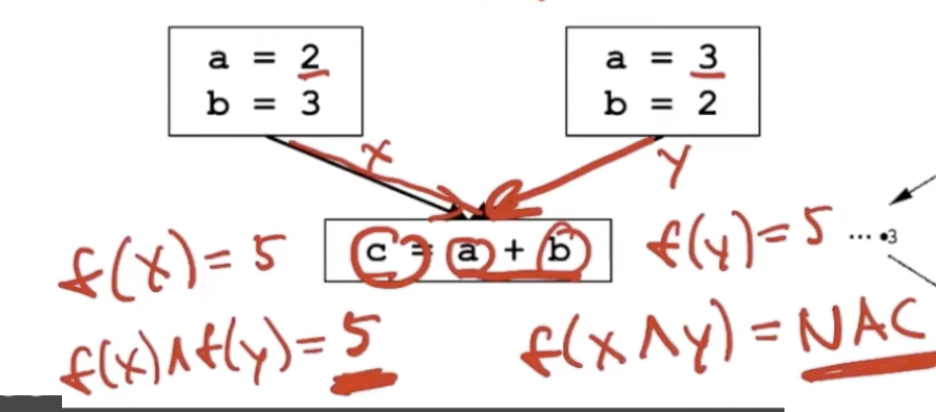
\includegraphics[width=0.2\textwidth]{CDp.png}
    \caption{}
    \label{fig:p15}
\end{figure}

\subsection{Data Flow Analysis}

\begin{definition}{Definition}
Let $f_1, \dots , f_m \in F$, where $f_i$ is the transfer function for node $i$. $f_p=f_{n_k} \cdot \ldots \cdot f_{n_1}$, where $p$ is a path through nodes $n_1  \cdot \ldots \cdot n_k$. $f_p =$ identify function, if $p$ is an empty path.
\end{definition}

\subsubsection{Precision}

Ideally for each node n, the IN should be $ \wedge f_{p_i}(\top)$ for all possibly executed path $p_i$ reaching n. But determining all possible executed paths is undecidable. Look at the example shown in \ref{fig:p20}.


\begin{figure}[h]
    \centering
    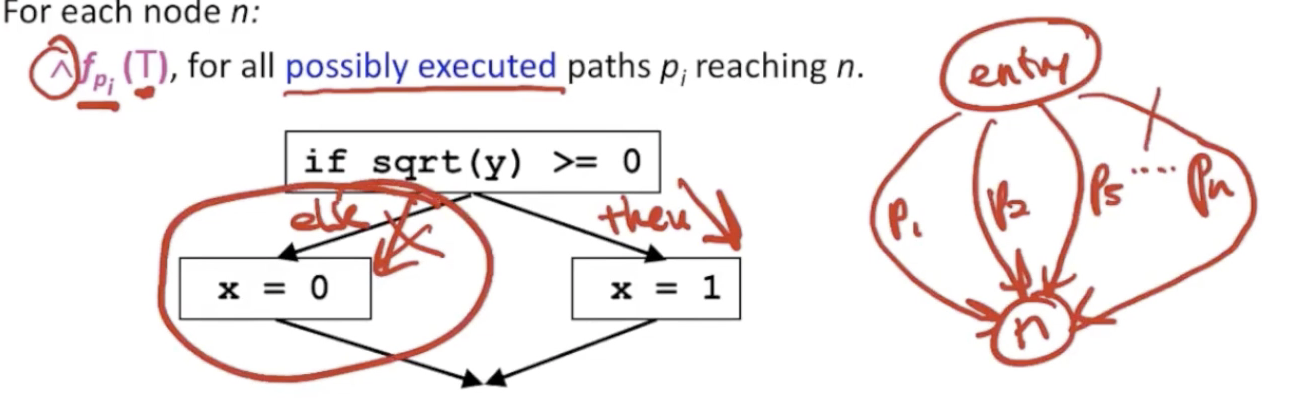
\includegraphics[width=0.2\textwidth]{p20.png}
    \caption{}
    \label{fig:p20}
\end{figure}

So in reality,  we will conservatively include some paths that will never be executed. From a correctness standpoint, this is fine because we will just get an more conservative answer.

\subsubsection{Meet-Over-Path(MOP)}

\begin{definition}{MOP}
For each node n, MOP(n) = $ \wedge f_{p_i}(\top)$ for all possibly executed path $p_i$ reaching n. 

Strictly speaking, MOP considers more paths than necessary, which means 

\[ \textit{MOP = Perfect-Solution} \wedge  \textit{Solution-to-Unexecuted-Paths.}\]

So 

\[ MOP \leq \textit{ Perfect-Solution} \]

MOP is more conservative. 

\end{definition}



\subsection{Solving Data Flow Equations}

Any solution that satisfies equations is a Fixed Point Solution(FP).


\subsubsection{Iterative algorithm }

If framework is monotone and algorithm coverges, then it computes Maximum Fixed Point(MFP).


FP $\leq$ MFP $\leq$ MOP $\leq$ Perfect-solution


Reaching Definition example:
\begin{figure}[h]
    \centering
    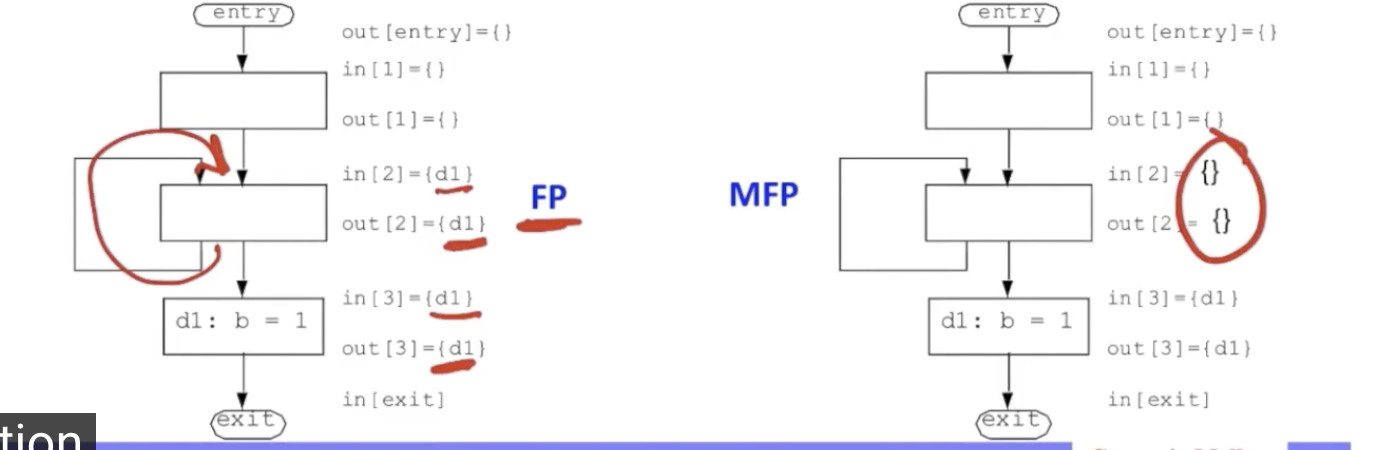
\includegraphics[width=0.2\textwidth]{p21.png}
    \caption{}
    \label{fig:p21}
\end{figure}




\subsection{Precision}

If data flow framework is distributive, then if the algorithm converges, $IN[b] = MOP[b]$

A Monotone but not distributive example: Constant Propagation.(Behaves as if there are additional paths)



\subsection{Convergence}
Properties are needed to guarantee convergence:

\begin{itemize}
    \item monotone
    \item finite descending chain
\end{itemize}



\subsection{Speed of Convergence}

\subsubsection{Reverse Post order}

\begin{figure}[h]
    \centering
    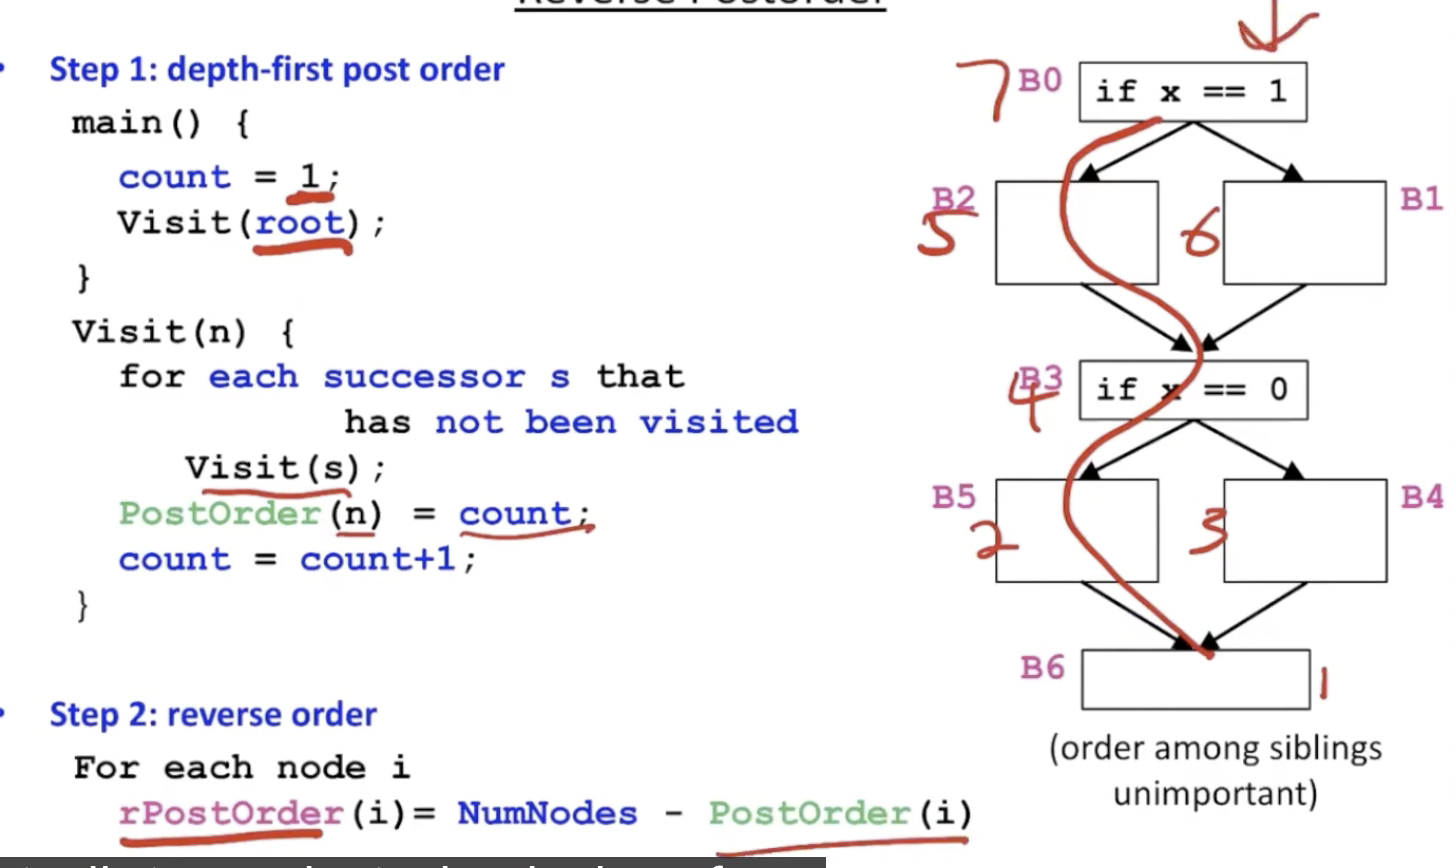
\includegraphics[width=0.2\textwidth]{p22.png}
    \caption{}
    \label{fig:p22}
\end{figure}


\subsubsection{Depth-First Iterative Algorithm(forward)
}



\begin{figure}[h]
    \centering
    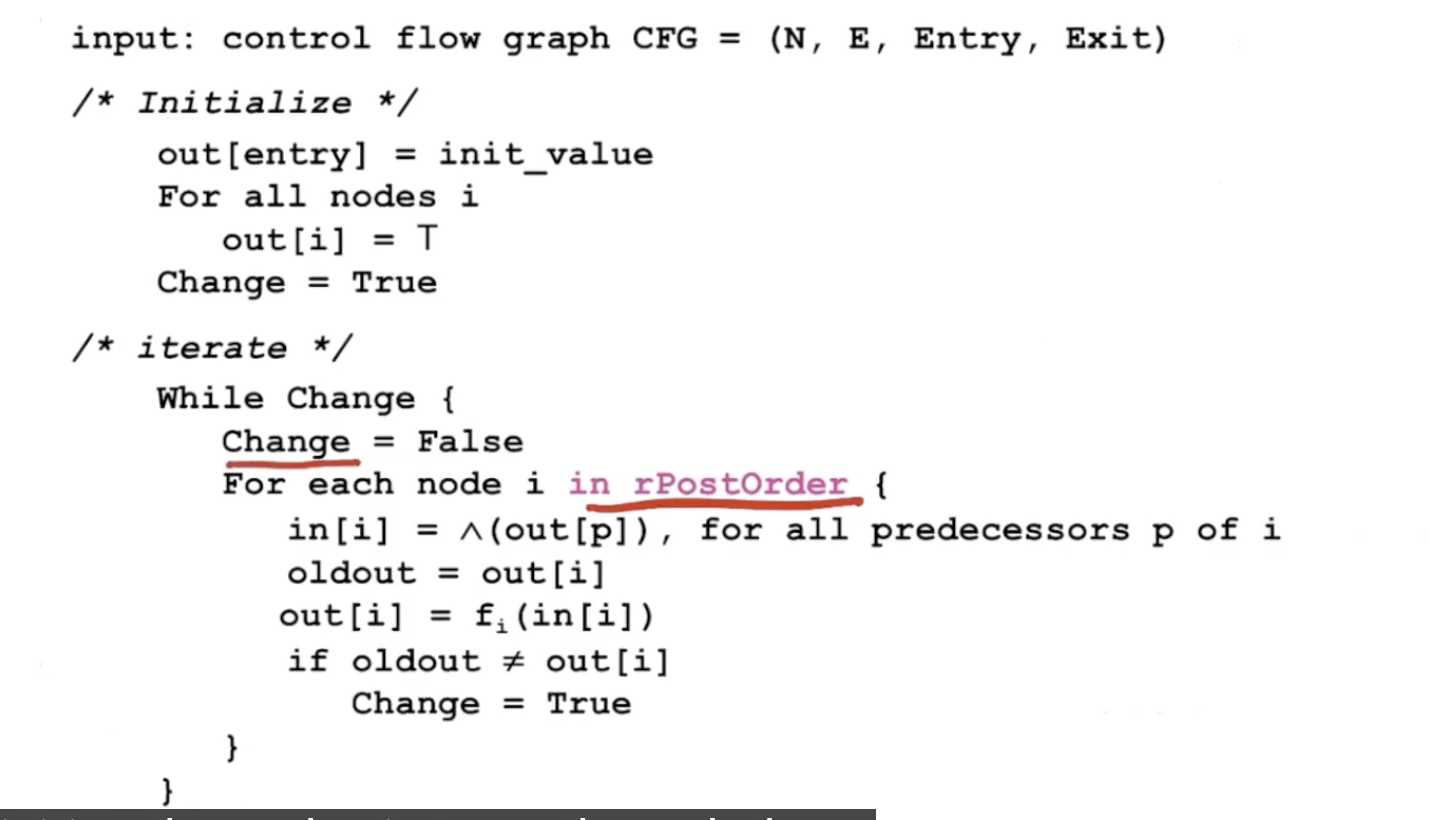
\includegraphics[width=0.2\textwidth]{p23.png}
    \caption{}
    \label{fig:p23}
\end{figure}


\subsubsection{Cost}

Number of iterations = number of back edges in any acyclic path +2 





% \section{More Examples of Data Flow Analysis: Global Common Sub-expression Elimination; Constant Propagation/Folding}

If we care about the past, what happened before, then it is a forward problem (entry). 


\subsection{Available Expression Analysis}


\begin{definition}{Availability of an Expression E at point P}
E is available at P if every path to P in the flow graph
\begin{itemize}
    \item E must be calculated at least once
    \item no variable in E redefined after the last evaluation

\end{itemize}
\end{definition}


\begin{figure}[h]
    \centering
    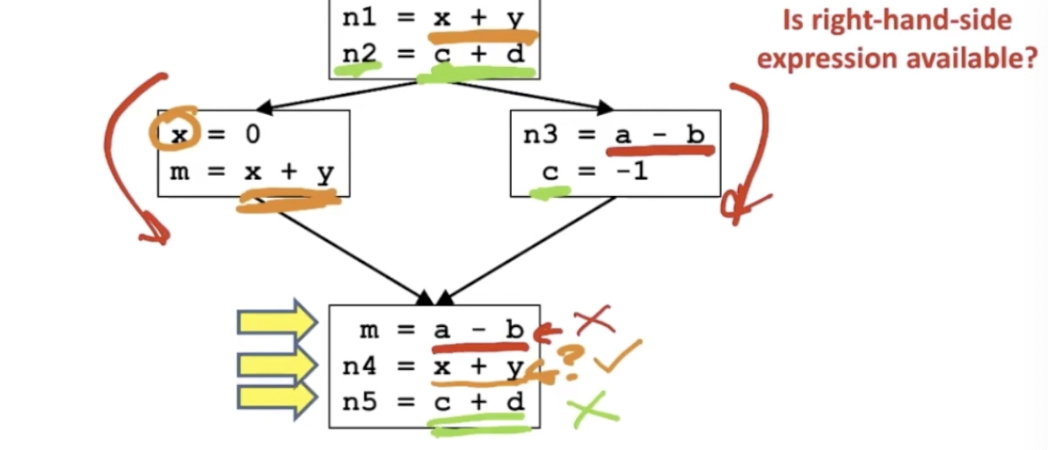
\includegraphics[width=0.3\textwidth]{p24.png}
    \caption{}
    \label{fig:p24}
\end{figure}


\subsubsection{Examples}



In \ref{fig:p24} $a-b$, $c+d$ is not available at the last BB. But $x+y$ is.


\begin{figure}[h]
    \centering
    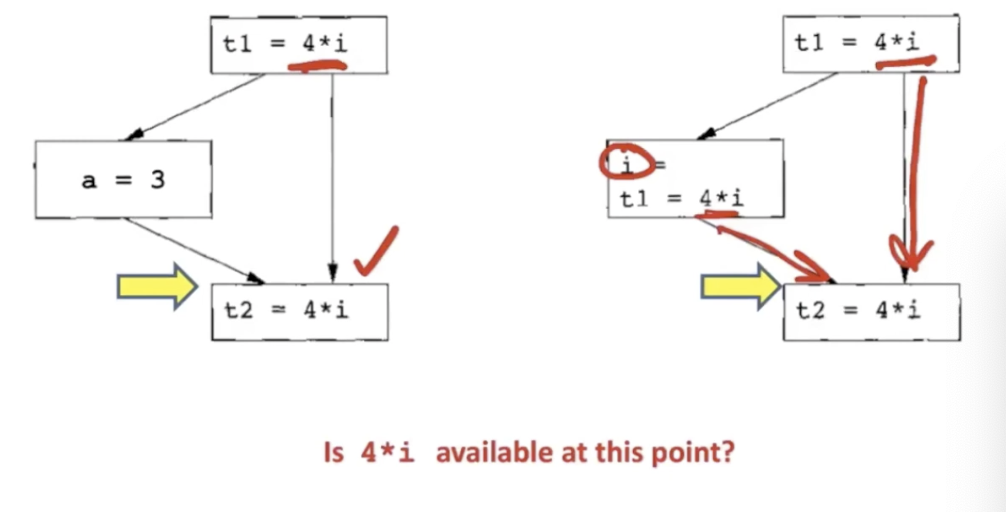
\includegraphics[width=0.3\textwidth]{p25.png}
    \caption{}
    \label{fig:p25}
\end{figure}


In \ref{fig:p25} , $4*i$ is available for both cases.



\begin{figure}[h]
    \centering
    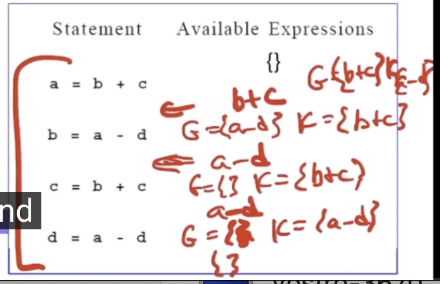
\includegraphics[width=0.3\textwidth]{p26.png}
    \caption{}
    \label{fig:p26}
\end{figure}


In \ref{fig:p26}, we show that calculate transfer functions for complete basic blocks by composing individual instruction transfer functions.


\begin{figure}[h]
    \centering
    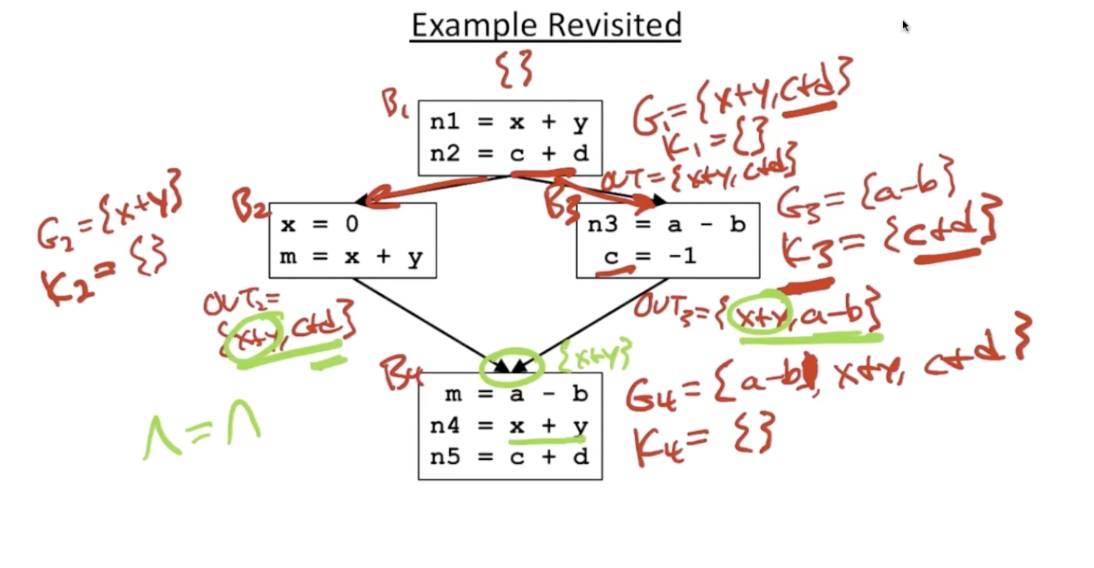
\includegraphics[width=0.3\textwidth]{p27.png}
    \caption{}
    \label{fig:p27}
\end{figure}


\subsection{Eliminating CSEs}


\begin{itemize}
    \item Step1: Value Numbering
    \item Step2: Available expression
    \item Step3: If CSE is an "available expression", then transform the code.
    
\end{itemize}

\begin{figure}[h]
    \centering
    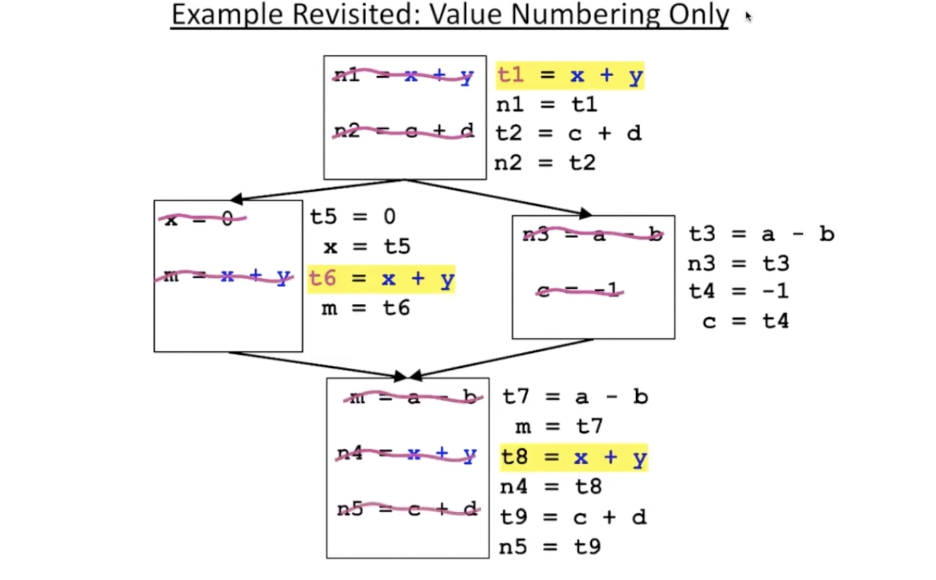
\includegraphics[width=0.3\textwidth]{p28.png}
    \caption{}
    \label{fig:p28}
\end{figure}

If we only use value numbering to eliminate common expression in \ref{fig:p28}, we will see that this will just add a lot of new work and no income. But if we calculate Available expression in \ref{fig:p29}, we can find that $x+y$ is such one and can do some optimization.


\begin{figure}[h]
    \centering
    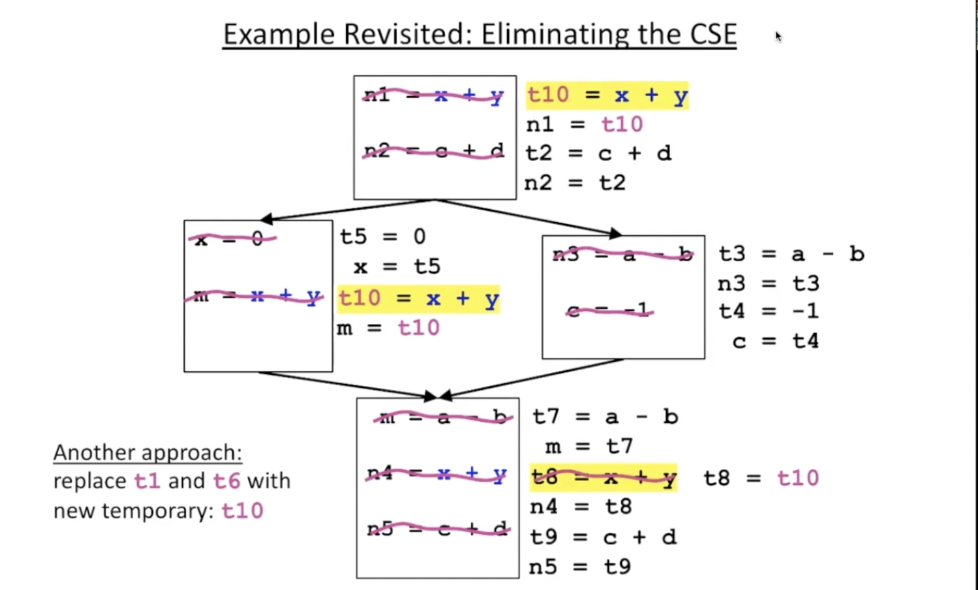
\includegraphics[width=0.3\textwidth]{p29.png}
    \caption{}
    \label{fig:p29}
\end{figure}

\begin{note}{How to deal with Textually identical expression?\ref{fig:p30}}
Just sort the operands.



But for textually different expressions that may be equivalent \ref{fig:p31}, we had better do copy propagation first.

\end{note}
\begin{figure}[h]
    \centering
    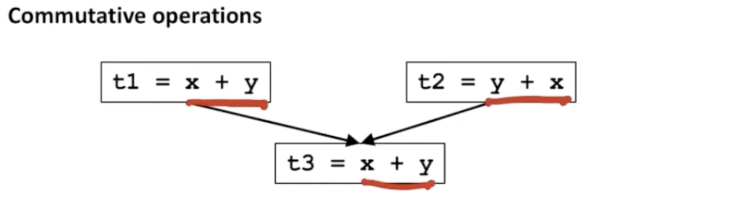
\includegraphics[width=0.3\textwidth]{p30.png}
    \caption{}
    \label{fig:p30}
\end{figure}

\begin{figure}[h]
    \centering
    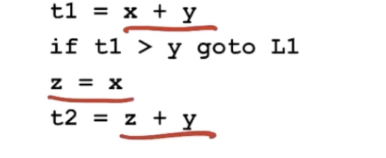
\includegraphics[width=0.3\textwidth]{p31.png}
    \caption{}
    \label{fig:p31}
\end{figure}


\subsubsection{Summary}

\begin{figure}[h]
    \centering
    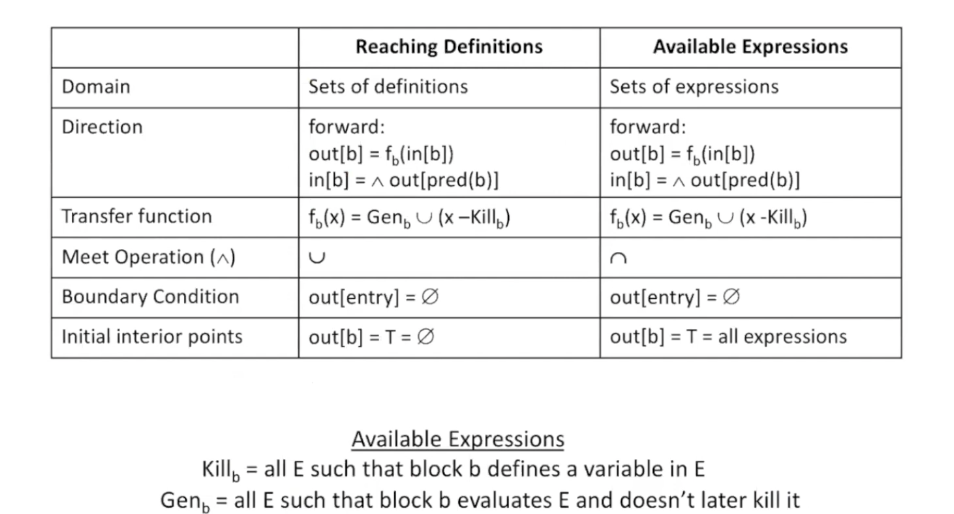
\includegraphics[width=0.3\textwidth]{p32.png}
    \caption{}
    \label{fig:p32}
\end{figure}


\subsection{Constant Propagation/Folding}

\begin{figure}[h]
    \centering
    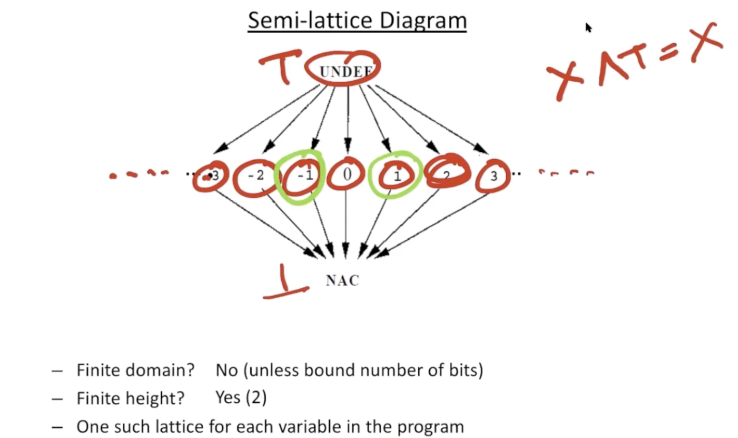
\includegraphics[width=0.3\textwidth]{p33.png}
    \caption{}
    \label{fig:p33}
\end{figure}

\subsubsection{Meet Operator in Table Form}
\begin{figure}[h]
    \centering
    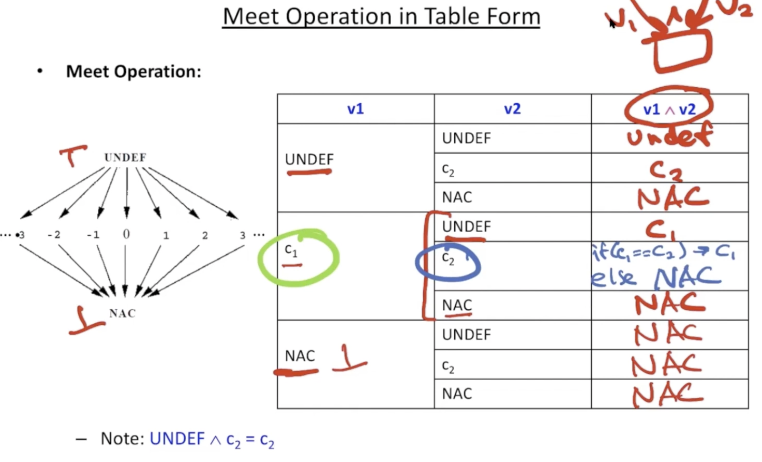
\includegraphics[width=0.3\textwidth]{p34.png}
    \caption{}
    \label{fig:p34}
\end{figure}


\subsubsection{Example}

\begin{figure}[h]
    \centering
    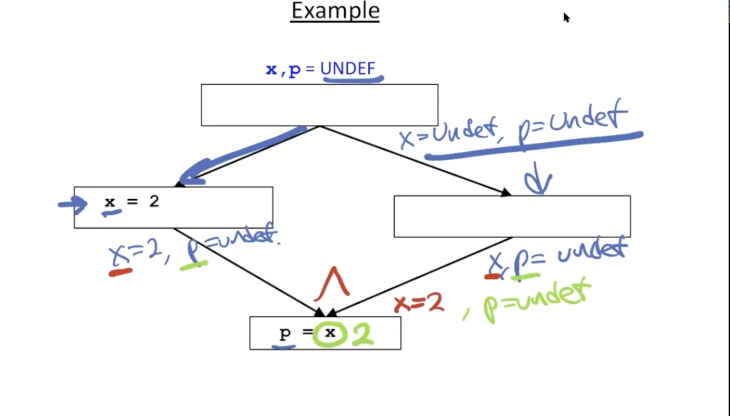
\includegraphics[width=0.3\textwidth]{p35.png}
    \caption{}
    \label{fig:p35}
\end{figure}

On the other path in \ref{fig:p35}, x is uninitialized. When we have undefined behavior, hopefully the front end of the compiler should complain about it, but if it doesn't, the optimizer is free to do whatever it wants to do.


\subsubsection{Transfer Function}


\begin{figure}[h]
    \centering
    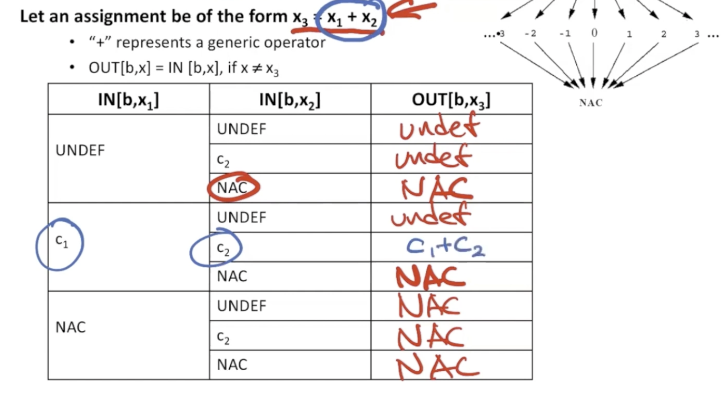
\includegraphics[width=0.3\textwidth]{p36.png}
    \caption{}
    \label{fig:p36}
\end{figure}



It is not distributive in \ref{fig:p37}.

\begin{figure}[h]
    \centering
    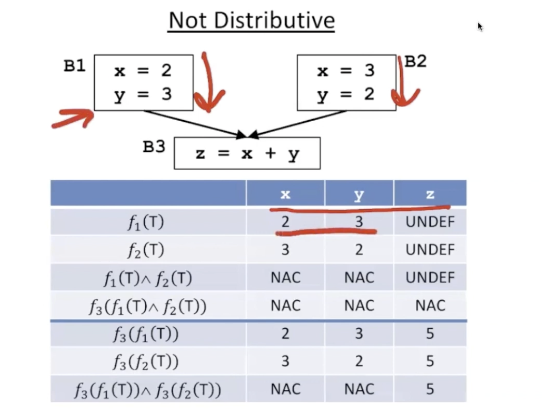
\includegraphics[width=0.3\textwidth]{p37.png}
    \caption{}
    \label{fig:p37}
\end{figure}



\subsection{Copy Propagation}

\subsection{Dead Code Elimination}




\section{Local Optimizations}

Local Optimizations never goes away because this is always a piece of what happens even when we 
talk about even more sophiscated types of optimizations.

First we will talk about how to represent the code within a function or procedure, that's using 
something called a flow graph which is made of basic blocks.  Next we will contrast two different 
abstractions for doing local optimizations.




\subsection{Basic Blocks/Flow graphs} 


\subsubsection{Basic Blocks}

A basic block is a sequence of instructions(3-address statements). There are some requirements for basic 
block:

\begin{itemize}
    \item \textbf{Only the first instruction can be reached from outside the blcok.} The reason why this property 
    is useful is that within a basic block, we just march instruction by instruction through the block, 
    this simplies things at least within a basic block.
    \item \textbf{All the statements are executed consecutively if the first one is.}
    \item \textbf{The basic block must be maximal.} i.e., they cannot be made larger without violating conditions. 
\end{itemize}


\subsubsection{Flow graphs}
Flow graph is a graph representation of the procedure. In flow graph, basic blocks are the nodes, and the edge for \(  B_i 
\rightarrow B_j \) stands for a path from node \( B_i \) to node \( B_j \). So how will \(  B_i  \rightarrow B_j \) happen? 
There are two possibilities:

\begin{itemize}
    \item Either first instruction of \(B_j\) is the target of a goto at end of \(B_i\).
    \item \(B_j\) physically follows \(B_i\) which doesn't end in an unconditional goto.
\end{itemize}




% \begin{center}

% \begin{tikzpicture}[auto,
%     node distance = 12mm,
%     start chain = going below,
%     box/.style = {draw,rounded corners,blur shadow,fill=white,
%           on chain,align=center}]
%    \node[box] (b1)    {$x_1\leftarrow0$\\ $y_1\leftarrow0$};      
%    \node[box] (b2)    {$x_2\leftarrow\phi(x_1,x_3)$\\
%    $y_2\leftarrow\phi(y_1,y_3)$\\
%    $(x_2<10)$?};      
%    \node[box] (b3)    {$y_3\leftarrow y_2+x_2$\\ $x_3\leftarrow x_2+1$};  
%    \node[box] (b4)    {print($y_2$)};     
%    \begin{scope}[rounded corners,-latex]
%     \path (b2.-40) edge[bend left=50] (b4.40)
%     (b1) edge (b2) (b2) edge (b3);
%     \draw (b3.230) -- ++(0,-0.3) -| ([xshift=-5mm]b2.west) |-
%     ([yshift=3mm]b2.130) -- (b2.130);
%    \end{scope}
%   \end{tikzpicture}

% \end{center}




\subsubsection{Partitioning into Basic Blocks}

\begin{itemize}
\item Identify the leader of each basic block 
    \begin{itemize}
        \item First instruction
        \item Any target of a jump
        \item Any instruction immediately following a jump
    \end{itemize}

\item Basic block starts at leader and ends at instruction immediately before a leader(or the last instruction).    
\end{itemize}

An example of flow graph is shown below:

\begin{figure}[h]
    \centering
    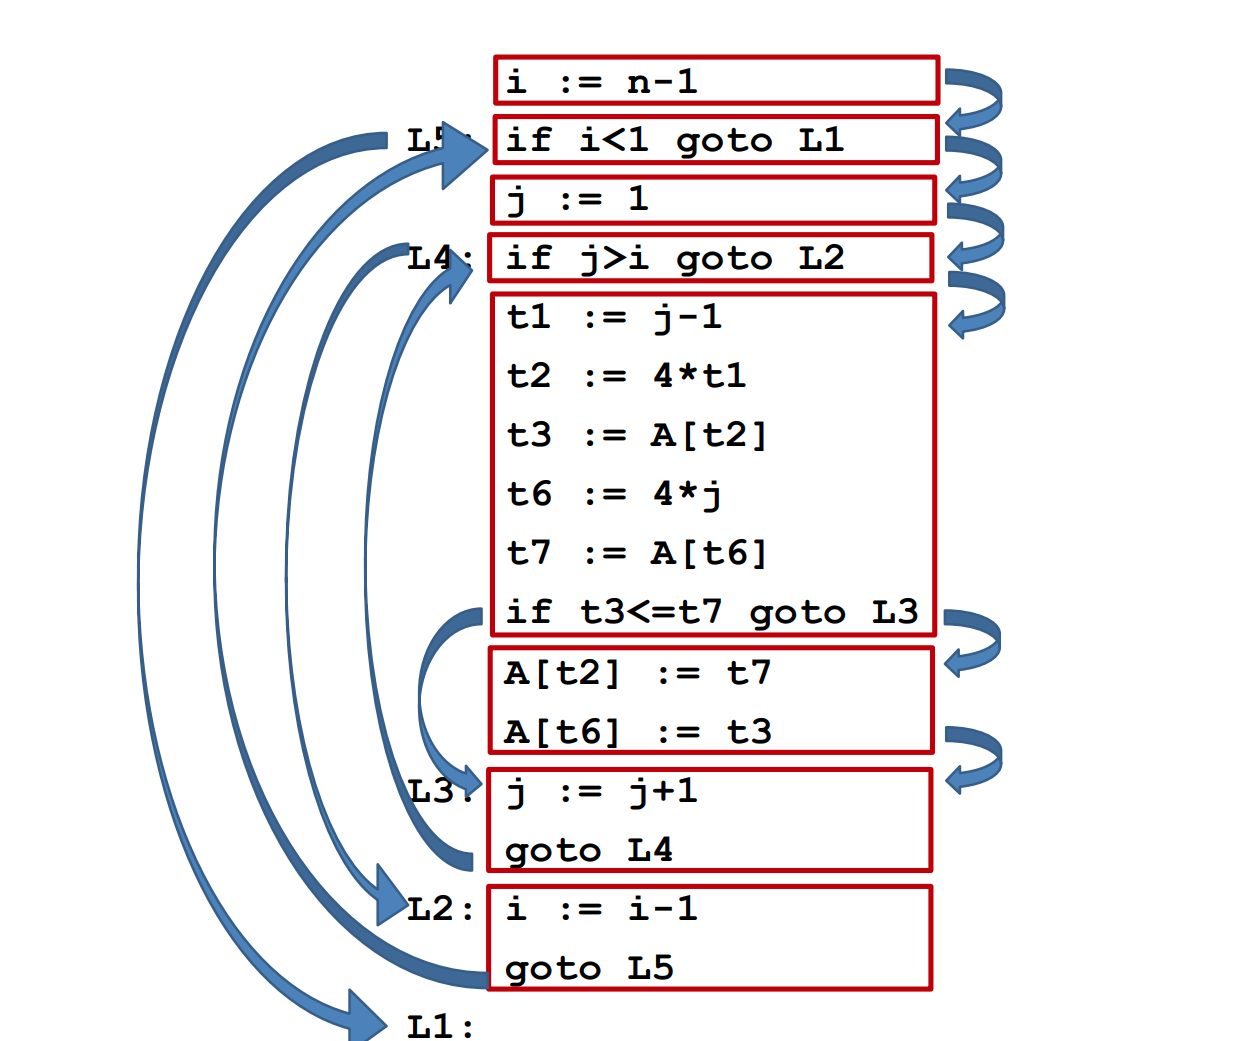
\includegraphics[width=0.5\textwidth]{flowgraph.png}
    \caption{Example of a flow graph}
\end{figure}

\subsubsection{Reachability of Basic Blocks}

There is one thing interesting need to mention here. So the source code is below:

\begin{lstlisting}[language=C, caption=An example]
if x { 
    ...
    return;
} else {
    ...
}


\end{lstlisting}


The corresponding flow graph is shown in \ref{fig:fgex}:

\begin{figure}[h]
    \centering
    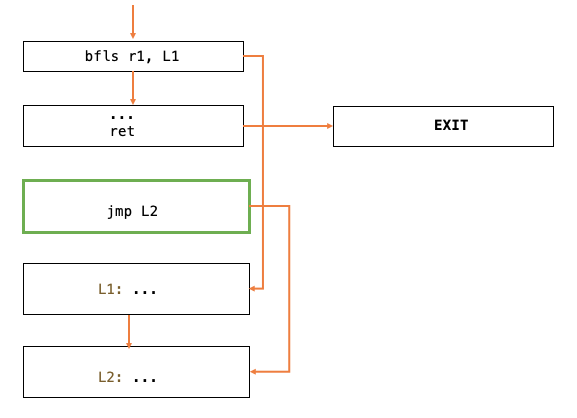
\includegraphics[width=0.5\textwidth]{fgex.png}
    \caption{Example of a flow graph}
    \label{fig:fgex}
\end{figure}


We can see that the box in green is unreachable from the entry. So why is that interesting? Typically, after compiers 
construct the control flow graph, they will go through and remove any unreachable nodes. Just do depth first traversal of the graph
from the entry node and mark all those visited nodes. So unmarked nodes will be deleted. This will help the compiler get a better optimization
result.


So why do these unreachable nodes appear? The anwser is it is not the job of the front-end of the compiler to clean up the unreachable nodes. 



\subsection{Local optimizations}

Local optimizations are those occur \textbf{within the basic blocks}. 


\subsubsection{common subexpression elimination}

There're some types of local optimizations. 
One is called \textbf{common subexpression elimination}. Subexpressions are some arithmetic expressions that occur on the
 right hand of the instructions. Common subexpressions are subexpression that occur many times where the operands have not 
 changed.
 
\begin{lstlisting}[language=C, caption=Subexpression example,label=lst:subexp]
a = b + c;
d = b + c;
\end{lstlisting}

In the example \ref{lst:subexp}, \texttt{b + c} is so called coomon subexpression, we could replace the instruction containing 
common subexpression with an assign expression. 


\begin{lstlisting}[language=C, caption=code snippet applied common subexpression elimination to \ref{lst:subexp},label=lst:transsubexpr]
    a = b + c;
    d = a
\end{lstlisting}

You may wonder why this kind of redundancy can occure in code? Are we programmers stupid to do so? In fact, 
the redundancy most comes from the stage when compilers  turn your source code. For example, when you use arrays,
you need to do some arithmetic to generate the address of the array element you are accessing. So every time you referece the same
array element, compiler will calculate the same address again. Similarly, if you access offsets within fields. Last example is 
access to parameters in the stack. 


\subsection{Abtraction 1:DAG}

DAG is the acronym for Directed Acyclic Graph. The Directed Acyclic Graph (DAG) is used to represent the 
structure of basic blocks, to visualize the flow of values between basic blocks, and to provide 
optimization techniques in the basic block. DAG is an efficient method for identifying common 
sub-expressions.\footnote{copied from \url{https://wildpartyofficial.com/what-is-dag-in-compiler-construction}}



The parse tree and DAG of the expression \(a + a*(b+c) + (b+c) *d \) is shown in \ref{fig:DAG}.


\begin{figure}[h]
    \centering
    \includegraphics[width=0.5\textwidth]{DAG.png}
    \caption{Example of a DAG}
    \label{fig:DAG}
\end{figure}



In DAG, some of the computation are reused. So we can generate optimizaed code based on DAG.

The optmized code for the DAG\ref{fig:DAG} is: 

\begin{lstlisting}[language=C, caption=code ,label=lst:dag]
    t1 = b - c;
    t2 = a * t1;
    t3 = a + t2;
    t4 = t1 * d;
    t5 = t3 + t4;
\end{lstlisting}


\subsubsection{How well do DAGs hold up across statements?}

We have seen that DAGs can be useful in a long arithmetic expression. So how well do DAGs
perform in sequence of instructions?

\begin{lstlisting}[language=C, caption=code ,label=lst:dagexpr2]
    a = b + c;
    b = a - d;
    c = b + c;
    d = a - d;
\end{lstlisting}


The corresponding DAG is shown in \ref{fig:DAG2}.
\begin{figure}[h]
    \centering
    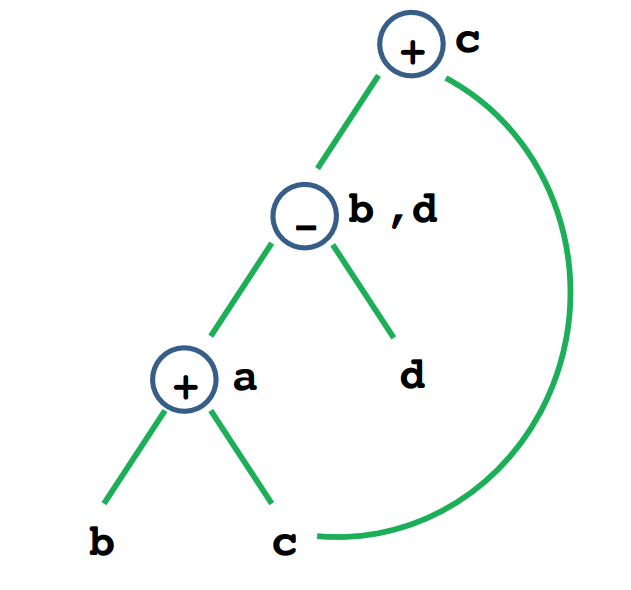
\includegraphics[width=0.5\textwidth]{dag2.png}
    \caption{Example of a DAG}
    \label{fig:DAG2}
\end{figure}

Based on the DAG\ref{fig:DAG2}, one optimizaed code is \ref{lst:dagexprop2}


\begin{lstlisting}[language=C, caption=code ,label=lst:dagexprop2]
a = b+c;
d = a-d;
c = d+c;
\end{lstlisting}

\ref{lst:dagexprop2} is not correct. B need to be overwritten but not yet. So if using DAGs, you need to be 
very careful. 

DAGs make sense if you just have one long expression, but once you have sequence of instructions overwriting variables
, DAGs are less appealing because this abstraction doesn't really include the concept of time.




\subsection{Abtraction 2:Value numbering} 

We have seen drawbacks of DAGs. One way to fix the problem is to attach variable name to latest value. Value numbering is 
such abstraction.

The idea behind value numbering is there is a mapping between variables(static) to values(dynamic). So common subexpression means same 
value number.

\subsubsection{Algorithm}


\begin{lstlisting}[language=python, caption=code ,label=lst:vna]
Data structure:
    VALUES = Table of
        expression /* [OP, valnum1, valnum2] */
        var /* name of variable currently holding expr */
For each instruction (dst = src1 OP src2) in execution order
    valnum1=var2value(src1); valnum2=var2value(src2)

    IF [OP, valnum1, valnum2] is in VALUES
        v = the index of expression
        Replace instruction with: dst = VALUES[v].var
    ELSE
        Add
            expression = [OP, valnum1, valnum2]
            var = tv
        to VALUES
        v = index of new entry; tv is new temporary for v
        Replace instruction with: tv = VALUES[valnum1].var OP VALUES[valnum2].var
                                dst = tv
    set_var2value (dst, v)  
\end{lstlisting}


\subsubsection{example}







\section{Introduction to Data Flow Analysis}

\subsection{Motivation for Dataflow Analysis}

Some optimizations\footnote{based on \url{https://pages.cs.wisc.edu/~horwitz/CS704-NOTES/2.DATAFLOW.html}} , however, require more "global" information. 
For example, consider the code \ref{lst:expr1}

\begin{lstlisting}[language=C,frame=single, caption=An ,label = lst:expr1]
    a = 1;
    b = 2;
    c = 3;
    if (...) x = a + 5;
    else x = b + 4;
    c = x + 1;
\end{lstlisting}


In this example, the initial assignment to \textit{c} (at line 3) is useless, and the expression 
\textit{x + 1} can be simplified to 7, but it is less obvious how a compiler can discover these facts 
since they cannot be discovered by looking only at one or two consecutive statements. 
A more global analysis is needed so that the compiler knows at each point in the program:
\begin{itemize}
\item    which variables are guaranteed to have constant values, and
\item    which variables will be used before being redefined.
\end{itemize}

To discover these kinds of properties, we use dataflow analysis. 



\subsubsection{What is Data Flow Analysis?}

Local Optimizations only consider optimizations within a node in CFG. 
Data flow analysis will take edges into account, which means composing 
effects of basic blocks to derive information at basic block boundaries.
Data-flow analysis is a technique for gathering information about the possible 
set of values calculated at various points in a computer program. A program's 
control-flow graph (CFG) is used to determine those parts of a program to which 
a particular value assigned to a variable might propagate. The information gathered 
is often used by compilers when optimizing a program. 


Typically, we will do local optimization for the first step to know what happens in a 
basic block, step 2 is to do data flow analysis. In he third step, we will go back and 
revisit the individual instructions inside of the blocks.


Data flow analysis is \textbf{flow-sensitive}, which means we take into account
 the effect of control flow. It is also a \textbf{intraprocedural analysis} which means
 the analysis is within a procedure. Data-flow analysis computes its solutions over the paths in
 a control-flow graph. The well-known, meet-over-all-paths
 formulation produces safe, precise solutions for general dataflow problems. All paths-whether feasible or infeasible,
 heavily or rarely executed-contribute equally to a solution. 

Here are some examples of intraprocedural optimizations:

\begin{itemize}
\item \textbf{constant propagation}. Constant propagation is a well-known global flow analysis 
problem. The goal of constant propagation is to discover values that are constant on all possible 
executions of a program and to propagate these constant values as far forward through the program 
as possible. Expressions whose operands are all constants can be evaluated at compile time and the 
results propagated further.

\item \textbf{common subexpression elimination}

\item \textbf{dead code elimination}. Actually, source code written by programmers doesn't contain
 a lot of dead code, dead code happens to occur partly because of how the front end translates code into 
 the IR. Doing optimizations will also turn code into dead.

\end{itemize}

% \subsection{Static    Program    vs.    Dynamic    Execution }

% Static program 




\subsubsection{Static Program vs. Dynamic Execution}


Program is statically infinite, but there can be infinite many dynamic execution paths. On one hand, analysis
 need to be precise, so we will take into account as much dynamic execution as possible. On the other hand, analysis
 need to do the analysis quickly. For a compromise, the analysis result is \textbf{conservative} and what it does id for each 
 point in the program, combines information of all the instances of the same program point.





\subsubsection{Data Flow Analysis Schema}
Before thinking about how to define a dataflow problem, note that there are two kinds of problems:
\begin{itemize}
    \item Forward problems (like constant propagation) where the information at a node n summarizes what can happen on paths from "enter" to n. So if we care about what happened in the past, it's a forward problem.
    \item Backward problems (like live-variable analysis), where the information at a node n summarizes what can happen on paths from n to "exit". So if we care about what will happen in the future, it's a backward problem.
\end{itemize}    

In what follows, we will assume that we're thinking about a forward problem unless otherwise specified.
 
Another way that many common dataflow problems can be categorized is as may problems or must problems. 
The solution to a "may" problem provides information about what may be true at each program point (e.g., 
for live-variables analysis, a variable is considered live after node n if its value may be used before 
being overwritten, while for constant propagation, the pair (x, v) holds before node n if x must have the value v at that point).

Now let's think about how to define a dataflow problem so that it's clear what the (best) solution should be. 
When we do dataflow analysis "by hand", we look at the CFG and think about:

\begin{itemize}
    \item What information holds at the start of the program.
    \item When a node n has more than one incoming edge in the CFG, how to combine the incoming 
    information (i.e., given the information that holds after each predecessor of n, how to 
    combine that information to determine what holds before n).
    \item How the execution of each node changes the information.
\end{itemize}    

This intuition leads to the following definition. An instance of a dataflow problem includes:
\begin{itemize}
    \item a \(CFG\),
    \item a domain \(D\) of "dataflow facts",
    \item a dataflow fact "init" (the information true at the start of the program for forward problems, 
    or at the end of the program for backward problems),
    \item an operator \(\wedge\) (used to combine incoming information from multiple predecessors),
    \item for each CFG node n, a dataflow function \(f_n\) :\( D \rightarrow D\) (that defines the effect of 
    executing n).
\end{itemize} 

For constant propagation, an individual dataflow fact is a set of pairs of the form (var, val),
 so the domain of dataflow facts is the set of all such sets of pairs (the power set). 
 For live-variable analysis, it is the power set of the set of variables in the program.

For both constant propagation and live-variable analysis, the "init" fact is the empty set 
(no variable starts with a constant value, and no variables are live at the end of the program).



For constant propagation, the combining operation \(\wedge\) is set intersection. 
This is because if a node n has two predecessors, p1 and p2, then variable x has value v before 
node n iff it has value v after both p1 and p2. For live-variable analysis, 
\(\wedge\) is set union: if a node n has two successors, s1 and s2, then the value of x after n may be 
used before being overwritten iff that holds either before s1 or before s2. In general, 
for "may" dataflow problems, \(\wedge\) will be some union-like operator, while it will be an intersection-like 
operator for "must" problems.

For constant propagation, the dataflow function associated with a CFG node that does not assign 
to any variable (e.g., a predicate) is the identity function. For a node n that assigns to 
a variable x, there are two possibilities:

\begin{itemize}
\item 1. The right-hand side has a variable that is not constant. In this case, the function 
result is the same as its input except that if variable x was constant the before n, 
it is not constant after n.
\item 2. All right-hand-side variables have constant values. In this case, the right-hand side of 
the assignment is evaluated producing consant-value c, and the dataflow-function result is the 
same as its input except that it includes the pair (x, c) for variable x (and excludes the pair 
for x, if any, that was in the input).
\end{itemize}


For live-variable analysis, the dataflow function for each node n has the form: 
\(f_n(S) = Gen_n \cup (S - KILL_n)\), where \(KILL_n\) is the set of variables defined at node n, 
and \(GEN_n\) is the set of variables used at node n. In other words, for a node that does not 
assign to any variable, the variables that are live before n are those that are live after 
n plus those that are used at n; for a node that assigns to variable x, the variables that are 
live before n are those that are live after n except x, plus those that are used at n 
(including x if it is used at n as well as being defined there).

An equivalent way of formulating the dataflow functions for live-variable analysis is: 
\(f_n(S) = (S \cap NOT-KILL_n) \cup GEN_n\), where \(NOT-KILL_n\) is the set of variables not defined
 at node n. The advantage of this formulation is that it permits the dataflow facts to be 
 represented using bit vectors, and the dataflow functions to be implemented using simple 
 bit-vector operations (and or).

It turns out that a number of interesting dataflow problems have dataflow functions of this 
same form, where \(GEN_n\) and \(KILL_n\) are sets whose definition depends only on n, and the combining 
operator \(\wedge\) is either union or intersection. These problems are called GEN/KILL problems, 
or bit-vector problems.




\subsection{Reaching Definitions}

The Reaching Definitions Problem is a data-flow problem used to answer the
following questions: Which definitions of a variable \textit{X} reach a given use of \textit{X} in
an expression? Is \textit{X} used anywhere before it is defined? A definition\textit{d} reaches a point \textit{p} if there exists path 
from the point immediately following \textit{d} to \textit{p} such that \textit{d} is not killed(overwritten) along that path.



\subsubsection{Iterative   Algorithm}

Here is the iterative  algorithm.



\begin{algorithm}
    \caption{Reaching Defintions:Iterative Algorithm}\label{alg:reachingdefiterative}
    \hspace*{\algorithmicindent} \textbf{Input: control flow graph CFG = (N, E, Entry, Exit) } \\
   
    
    \begin{algorithmic}
   
    \State out[Entry] = $\emptyset$ \algorithmiccomment{Boundary condition}

    \For{\texttt{each basic block B other than Entry}}
        \State \texttt{out[B] = $\emptyset$} \algorithmiccomment{Initialization for iterative algorithm }
    \EndFor
    \While{Changes to any out[] occur}
        \For{\texttt{each basic block B other than Entry}}
        \State \texttt{$in[B] =  \cup (out[p])$, for all predecessors p of B}
        \State \texttt{$out[B] = f_B(in[B])$} \algorithmiccomment{$out[B]=gen[B]\cup (in[B]-kill[B]) $ }
        \EndFor

    \EndWhile
    \end{algorithmic}
\end{algorithm}




\subsubsection{ Worklist   Algorithm}

\begin{algorithm}
    \caption{Reaching Defintions:Worklist Algorithm}\label{alg:reachingdefiterative}
    \hspace*{\algorithmicindent} \textbf{Input: control flow graph CFG = (N, E, Entry, Exit) } \\
   
    
    \begin{algorithmic}
   
    \State out[Entry] = $\emptyset$ \algorithmiccomment{Boundary condition}
    \State \textcolor{blue}{ChangedNodes = N}   
    \For{\texttt{each basic block B other than Entry}}
        \State \texttt{out[B] = $\emptyset$} \algorithmiccomment{Initialization for iterative algorithm }
    \EndFor
    \While{ChangedNodes $\neq \emptyset$}
        \State \textcolor{blue}{Remove i from ChangedNodes}
        \State $in[B] =  \cup (out[p])$, for all predecessors p of B
        \State \textcolor{blue}{$oldout = out[i]$}
        \State $out[i] = f_i(in[i])$ \algorithmiccomment{$out[i]=gen[i]\cup (in[i]-kill[i]) $ }
        \If {\textcolor{blue}{oldout} $\neq out[i]$}

            \For{\texttt{all \textcolor{blue}{successors s of i}}}
                \State \textcolor{blue}{add s to ChangedNodes}
            \EndFor
        \EndIf

    \EndWhile
    \end{algorithmic}
\end{algorithm}



\subsubsection{Example}


\begin{figure}[!htb]
    \minipage{0.32\textwidth}
      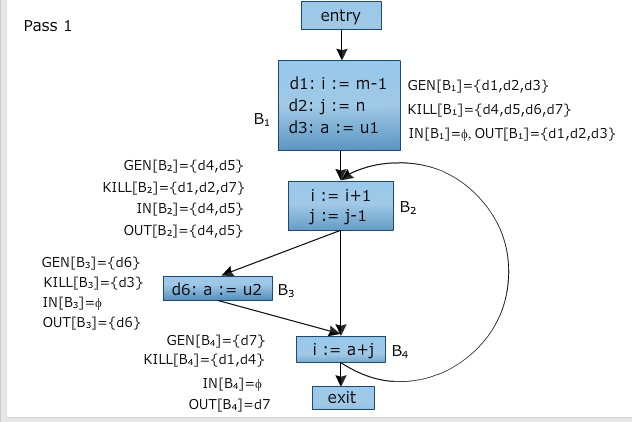
\includegraphics[width=\linewidth]{rdex1.jpg}
      \caption{Pass 1}\label{fig:awesome_image1}
    \endminipage\hfill
    \minipage{0.32\textwidth}
      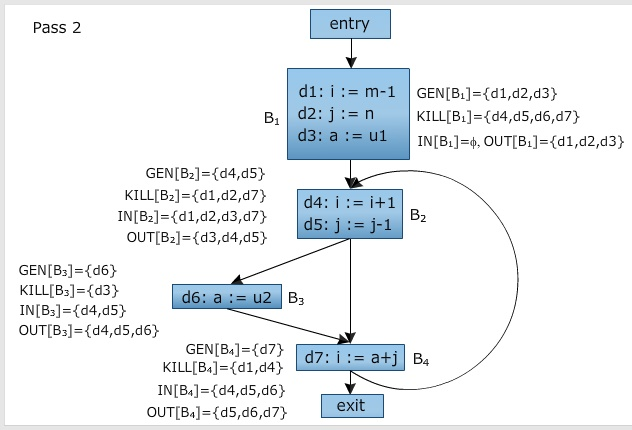
\includegraphics[width=\linewidth]{rdex2.jpg}
      \caption{Pass 2}\label{fig:awesome_image2}
    \endminipage\hfill
    \minipage{0.32\textwidth}%
      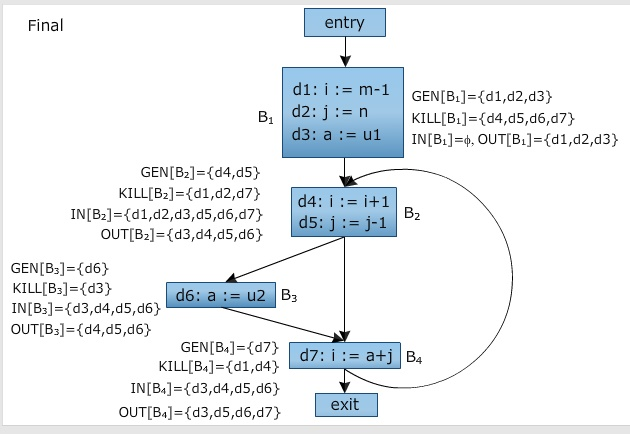
\includegraphics[width=\linewidth]{rdex3.jpg}
      \caption{Pass 3}\label{fig:awesome_image3}
    \endminipage
\end{figure}



\subsection{ Live    Variable    Analysis   }

In compilers, live variable analysis (or simply liveness analysis)
 is a classic data-flow analysis to calculate the variables that 
 are live at each point in the program. A variable is live at 
 some point if it holds a value that may be needed in the future, 
 or equivalently if its value may be read before the next time 
 the variable is written to. \footnote{based on Wikipedia}

\subsubsection{Motivation}


For dead code elimination.
\subsection{}


\section{Reaching Definitions}

The Reaching Definitions Problem is a data-flow problem used to answer the
following questions: Which definitions of a variable \textit{X} reach a given use of \textit{X} in
an expression? Is \textit{X} used anywhere before it is defined? A definition\textit{d} reaches a point \textit{p} if there exists path 
from the point immediately following \textit{d} to \textit{p} such that \textit{d} is not killed(overwritten) along that path.



\subsection{Iterative   Algorithm}

Here is the iterative  algorithm.



\begin{algorithm}
    \caption{Reaching Defintions:Iterative Algorithm}\label{alg:reachingdefiterative}
    \hspace*{\algorithmicindent} \textbf{Input: control flow graph CFG = (N, E, Entry, Exit) } \\
   
    
    \begin{algorithmic}
   
    \State out[Entry] = $\emptyset$ \algorithmiccomment{Boundary condition}

    \For{\texttt{each basic block B other than Entry}}
        \State \texttt{out[B] = $\emptyset$} \algorithmiccomment{Initialization for iterative algorithm }
    \EndFor
    \While{Changes to any out[] occur}
        \For{\texttt{each basic block B other than Entry}}
        \State \texttt{$in[B] =  \cup (out[p])$, for all predecessors p of B}
        \State \texttt{$out[B] = f_B(in[B])$} \algorithmiccomment{$out[B]=gen[B]\cup (in[B]-kill[B]) $ }
        \EndFor

    \EndWhile
    \end{algorithmic}
\end{algorithm}




\subsection{ Worklist   Algorithm}

\begin{algorithm}
    \caption{Reaching Defintions:Worklist Algorithm}\label{alg:reachingdefiterative}
    \hspace*{\algorithmicindent} \textbf{Input: control flow graph CFG = (N, E, Entry, Exit) } \\
   
    
    \begin{algorithmic}
   
    \State out[Entry] = $\emptyset$ \algorithmiccomment{Boundary condition}
    \State \textcolor{blue}{ChangedNodes = N}   
    \For{\texttt{each basic block B other than Entry}}
        \State \texttt{out[B] = $\emptyset$} \algorithmiccomment{Initialization for iterative algorithm }
    \EndFor
    \While{ChangedNodes $\neq \emptyset$}
        \State \textcolor{blue}{Remove i from ChangedNodes}
        \State $in[B] =  \cup (out[p])$, for all predecessors p of B
        \State \textcolor{blue}{$oldout = out[i]$}
        \State $out[i] = f_i(in[i])$ \algorithmiccomment{$out[i]=gen[i]\cup (in[i]-kill[i]) $ }
        \If {\textcolor{blue}{oldout} $\neq out[i]$}

            \For{\texttt{all \textcolor{blue}{successors s of i}}}
                \State \textcolor{blue}{add s to ChangedNodes}
            \EndFor
        \EndIf

    \EndWhile
    \end{algorithmic}
\end{algorithm}



\subsection{Example}
Here comes an example of reaching definition.

\begin{figure}[!htb]
    \minipage{0.32\textwidth}
      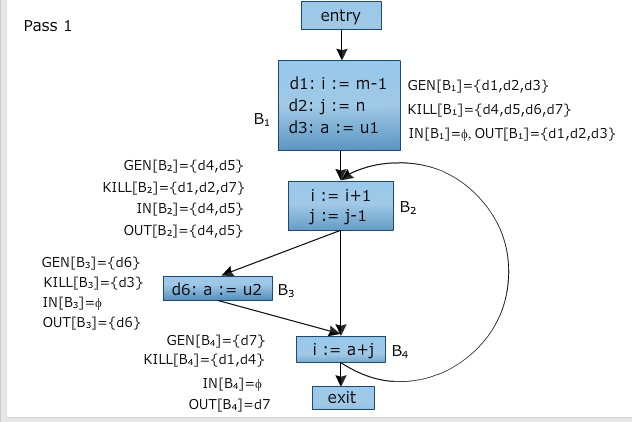
\includegraphics[width=\linewidth]{rdex1.jpg}
      \caption{Pass 1}\label{fig:awesome_image1}
    \endminipage\hfill
    \minipage{0.32\textwidth}
      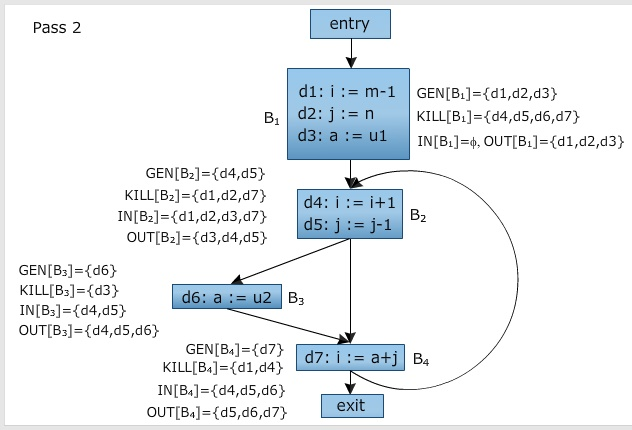
\includegraphics[width=\linewidth]{rdex2.jpg}
      \caption{Pass 2}\label{fig:awesome_image2}
    \endminipage\hfill
    \minipage{0.32\textwidth}%
      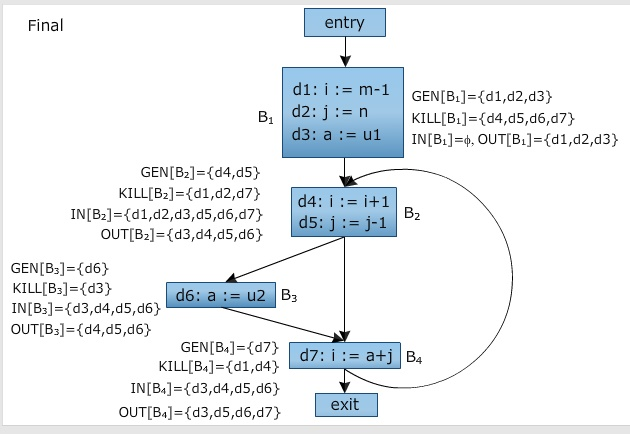
\includegraphics[width=\linewidth]{rdex3.jpg}
      \caption{Pass 3}\label{fig:awesome_image3}
    \endminipage
\end{figure}
\section{ Live Variabl Analysis   }

In compilers, live variable analysis (or simply liveness analysis)
is a classic data-flow analysis to calculate the variables that
are live at each point in the program. A variable is live at
some point if it holds a value that may be needed in the future,
or equivalently if its value may be read before the next time
the variable is written to. \footnote{based on Wikipedia}

\subsection{Motivation}

Programs may contain

\begin{itemize}
	\item code which gets executed but which has no useful
	      effect on the program's overall result;
	\item occurrences of variables being used before they
	      are defined;\footnote{we can use liveness information to find undefined variables.}
	\item many variables which need to be allocated
	      registers and/or memory locations for compilation.\footnote{Two	variables	can	use	the	same	register	if	they	are	never	in	use	at	the
		      same time(i.e,	never	simultaneously live). Register	allocation
		      uses liveness information.}

\end{itemize}

The concept of variable liveness is useful in dealing
with all three of these situations.


Liveness analysis is highly used for \textbf{register allocation}(If variable \texttt{x} is live in a basic block b, it is a potential candidate for
register allocation) and \textbf{dead code elimination}(If variable \texttt{x} is not live after an assignment \texttt{x =...}, then the assignment is
redundant and can be deleted as dead code).


\subsection{Problem formulation}
Liveness is a data-flow property of variables:
“Is the value of this variable needed?” We therefore
usually consider liveness from an instruction's
perspective: each instruction (or node of the
flowgraph) has an associated set of live variables.


\subsection{Semantic vs. syntactic}


There are two kinds of variable liveness : Semantic liveness and Syntactic liveness.


A variable x is \textbf{semantically} live at a node n if there is
some execution sequence starting at n whose (externally
observable) behaviour can be affected by changing the
value of x. Semantic liveness is concerned with
the execution behaviour of the program.

A variable is \textbf{syntactically} live at a node if there is a
path to the exit of the flow graph along which its
value may be used before it is redefined. Syntactic liveness is concerned with properties of
the syntactic structure of the program.


So what is the difference between Semantic liveness and Syntactic liveness? syntactic liveness
is a computable approximation of semantic liveness.


Consider the example \ref{lst:expr2}


\begin{lstlisting}[language=C,frame=single, caption=An example to illustrate semantic syntatic,label = lst:expr2]
    int t = x * y;
    if ((x+1)*(x+1) == y) {
     t = 1;
    }
    if (x*x + 2*x + 1 != y) {
     t = 2;
    }
    return t;
\end{lstlisting}

In fact, t is dead in node \texttt{int t = x * y;} because one of the conditions will be true,
so on every execution path t is redefined before it is returned.
The value assigned by the first instruction is never used.


But on read path from Figure \ref{fig:liveex} through the
flowgraph, t is not
redefined before it's used,
so t is syntactically live at
the first instruction.Note that this path never
actually occurs during
execution.

\begin{figure}[h]
	\centering
	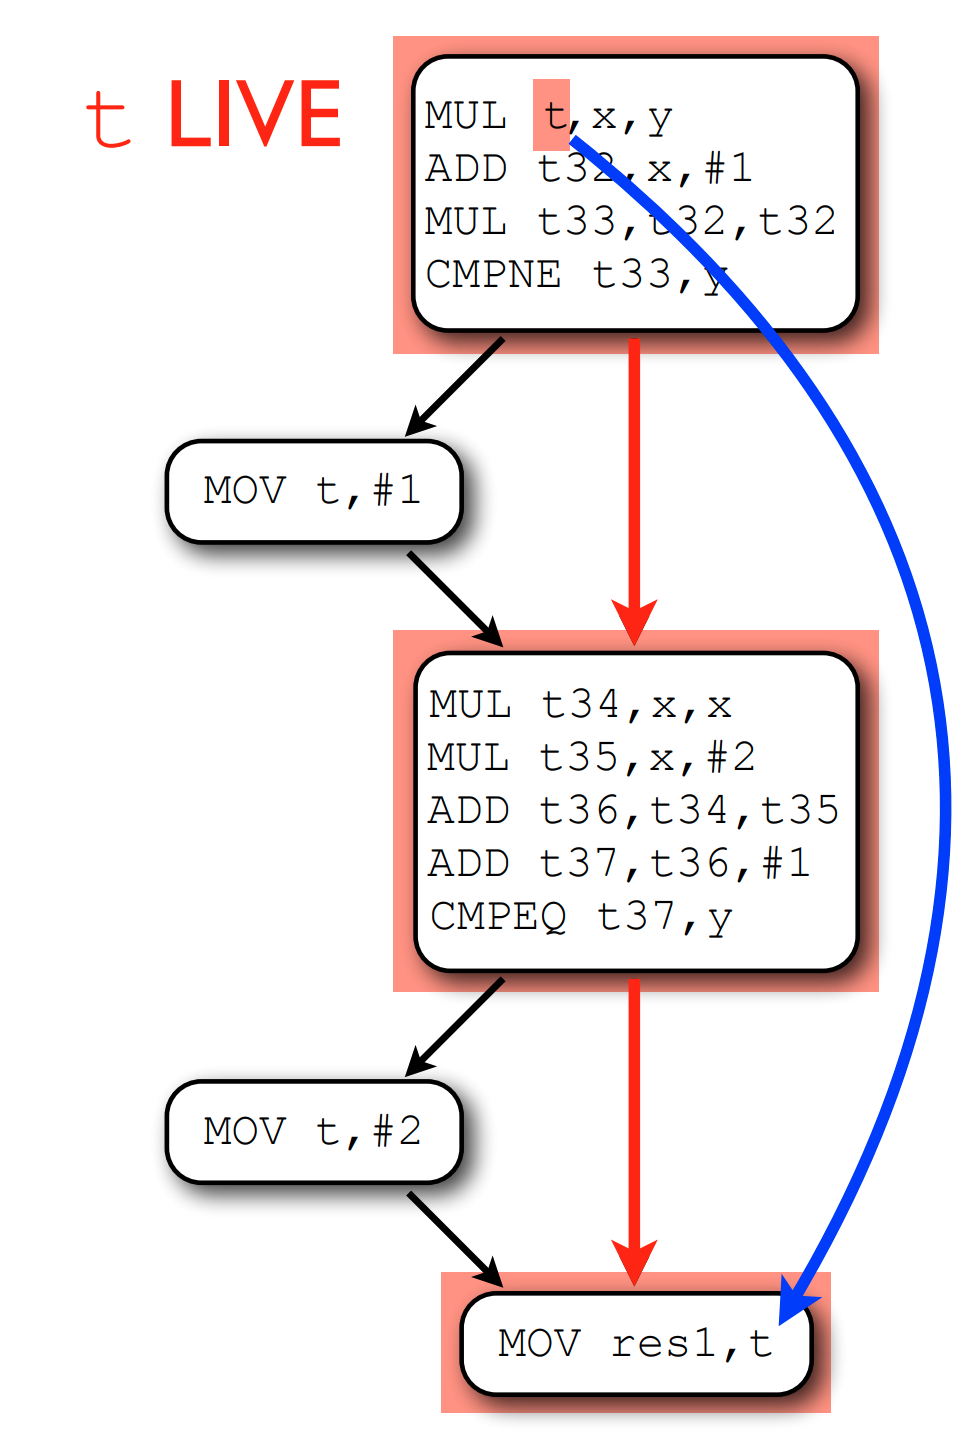
\includegraphics[width=0.3\textwidth]{liveex.png}
	\caption{CFG for \ref{lst:expr2}}
	\label{fig:liveex}
\end{figure}


\subsection{Summary}


\begin{center}
	\begin{tabular}{|c|c|}
		\hline Direction                         & Backward                                            \\
		\hline Domain                            & Sets	of	variables                                     \\
		\hline Meet operator                     & \( \cup \)                                          \\
		\hline Top(T)                            & $\phi$                                              \\
		\hline Bottom                            & Universal Set                                       \\
		\hline Boundary condition                & $\mathrm{IN[EXIT]} = \phi$                          \\
		\hline Initialization for internal nodes & $\mathrm{IN[B]} = \phi$                             \\
		\hline Finited escending chain?          & \checkmark                                          \\
		\hline Transfer function                 & $f_b(x) = \mathrm{USE}_b \cup (x - \mathrm{DEF}_b)$ \\
		\hline Monotone\&Distributive?           & \checkmark                                          \\
		\hline
	\end{tabular}
\end{center}




\subsection{Strongly Live Variables Analysis\cite{LiveVari29:online}}

A variable is strongly live if
\begin{itemize}

	\item it is used in a statement other than assignment statement, or
	      (same as simple liveness)
	\item it is used in an assignment statement defining a variable that is
	      strongly live
\end{itemize}


\begin{figure}[H]
	\centering
	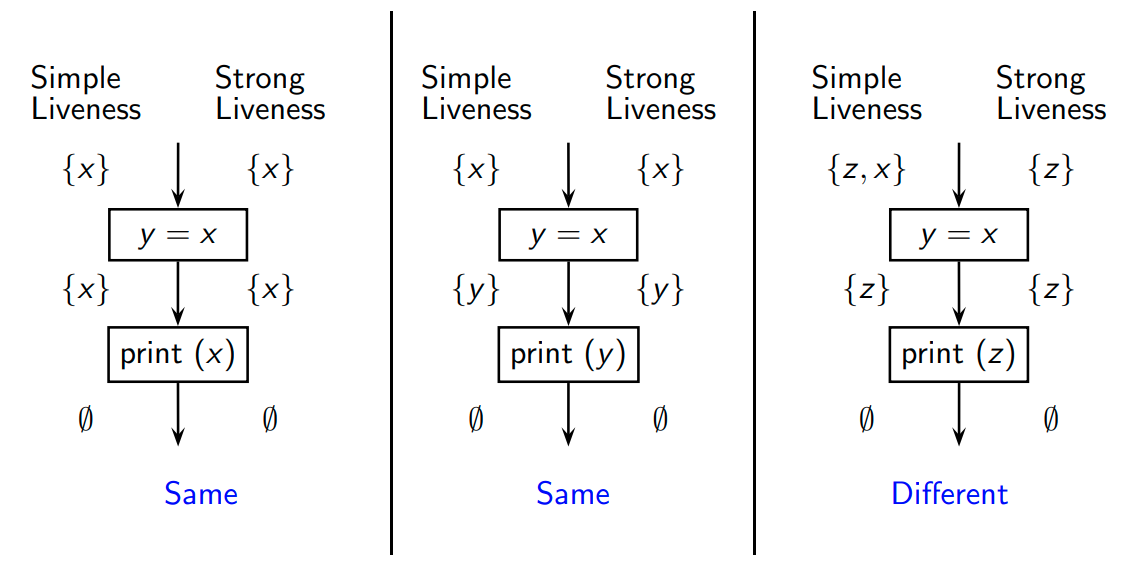
\includegraphics[width=0.7\textwidth]{p217.png}
	\caption{Understanding Strong Liveness}
	\label{fig:p217}
\end{figure}


A variable is live at a program
point if its current value is likely
to be used later. We want to compute the smallest
set of variables that are live. Simple liveness considers every
use of a variable as useful. Strong liveness checks the liveness
of the result before declaring the
operands to be live. Strong liveness is more precise
than simple liveness. The transfer function of Strongly Live Variables Analysis is shwon
below:


$$
	f_n(X)= \begin{cases}(X-\{y\}) \cup(Opd(e) \cap \mathbb{V}ar) & n \text { is } y=e, e \in \mathbb{E}pr, y \in X \\ X-\{y\} & n \text { is input }(y) \\ X \cup\{y\} & n \text { is use }(y) \\ X & \text { otherwise }\end{cases}
$$


The first case means that If \texttt{y} is not strongly live, the
assignment is skipped using
the “otherwise” clause

\begin{figure}[H]
	\centering
	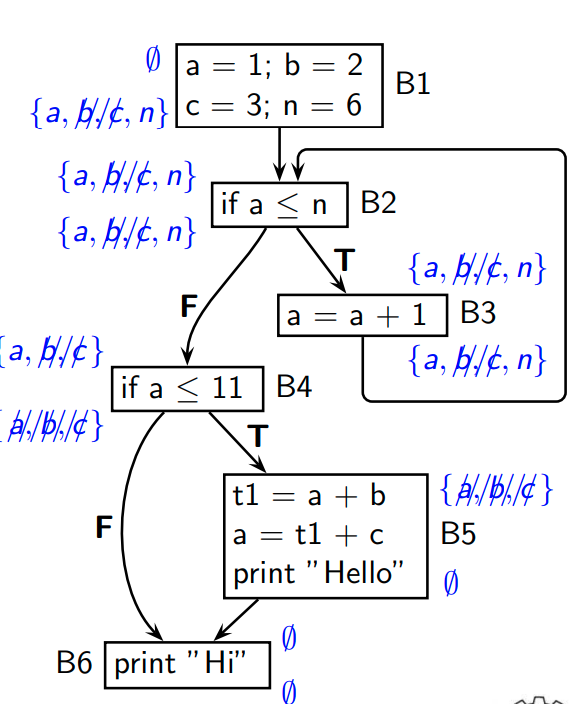
\includegraphics[width=0.4\textwidth]{p218.png}
	\caption{Simple Liveness VS. Strong Liveness.}
	\label{fig:p218}
\end{figure}

\newpage

\section{Available Expressions Analysis}

\subsection{Motivation}

Programs may contain code whose result is needed, but in which some computation is simply a redundant
repetition of earlier computation within the same program. The concept of expression availability is useful in dealing with this situation.


\subsection{Backgroud Knowledge}

Any given program contains a finite number of expressions (i.e. computations which potentially
produce values),so we may talk about the set of all expressions of a program. Consider the program in
\ref{lst:expression1}




\begin{lstlisting}[language=C,frame=single, caption=An simple example containing some expressions ,label = lst:expression1]
    int z = x * y; 
    print s + t; 
    int w = u / v;
\end{lstlisting}


This program contian expression \texttt{x*y,s+t,u/v}.



\subsection{Problem Formulation}


Availability is a data-flow property of expressions: “Has the value of this expression already been computed?”
At each instruction, each expression in the programis either available or unavailable. So each instruction(or node of the flowgraph) has
an associated set of available expression.



\subsection{Semantic vs. Syntactic}

An expression is \textit{semantically} available at a node n if its value gets computed
(and not subsequently invalidated) along every execution sequence ending at n.

\begin{figure}[!htb]
	\minipage{0.5\textwidth}
	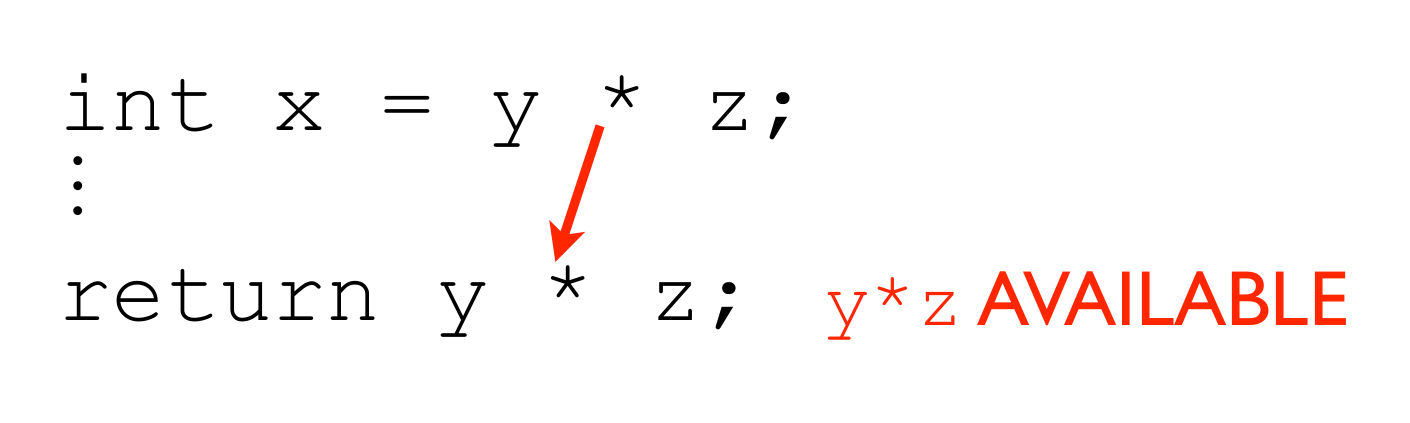
\includegraphics[width=\linewidth]{p1.png}
	\caption{Available expression example}\label{fig:p1}
	\endminipage\hfill
	\minipage{0.5\textwidth}
	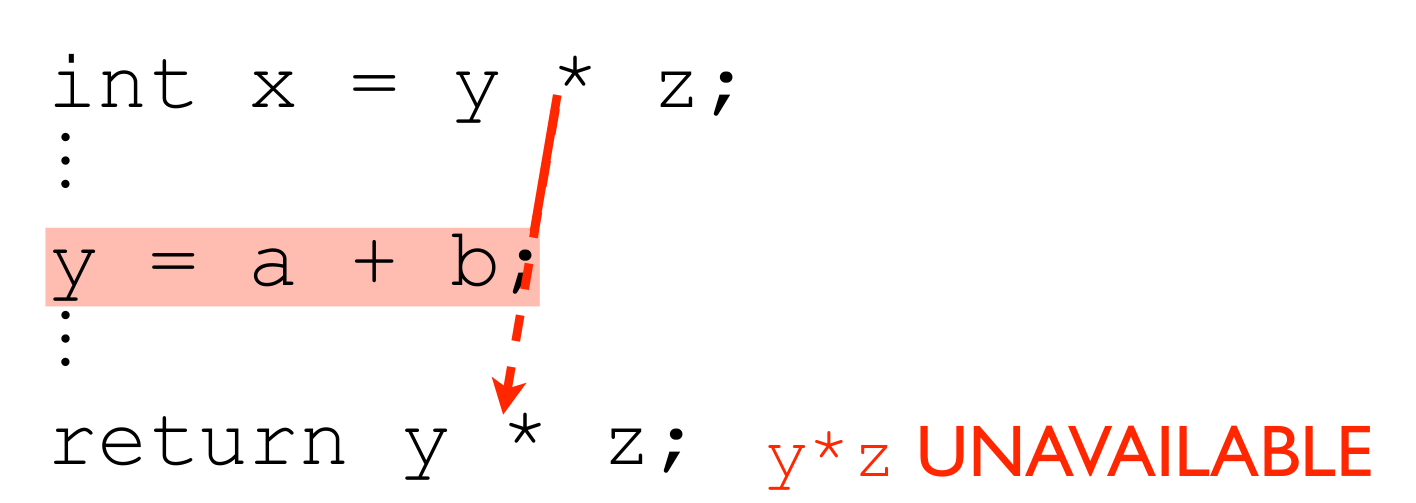
\includegraphics[width=\linewidth]{p2.png}
	\caption{unavailable expression example}\label{fig:p2}
	\endminipage
\end{figure}


An expression is \textit{syntactically} available at a node n if its value gets computed
(and not subsequently invalidated) along every path from the entry of the flowgraph to n.


\begin{figure}[!htb]
	\minipage{0.5\textwidth}
	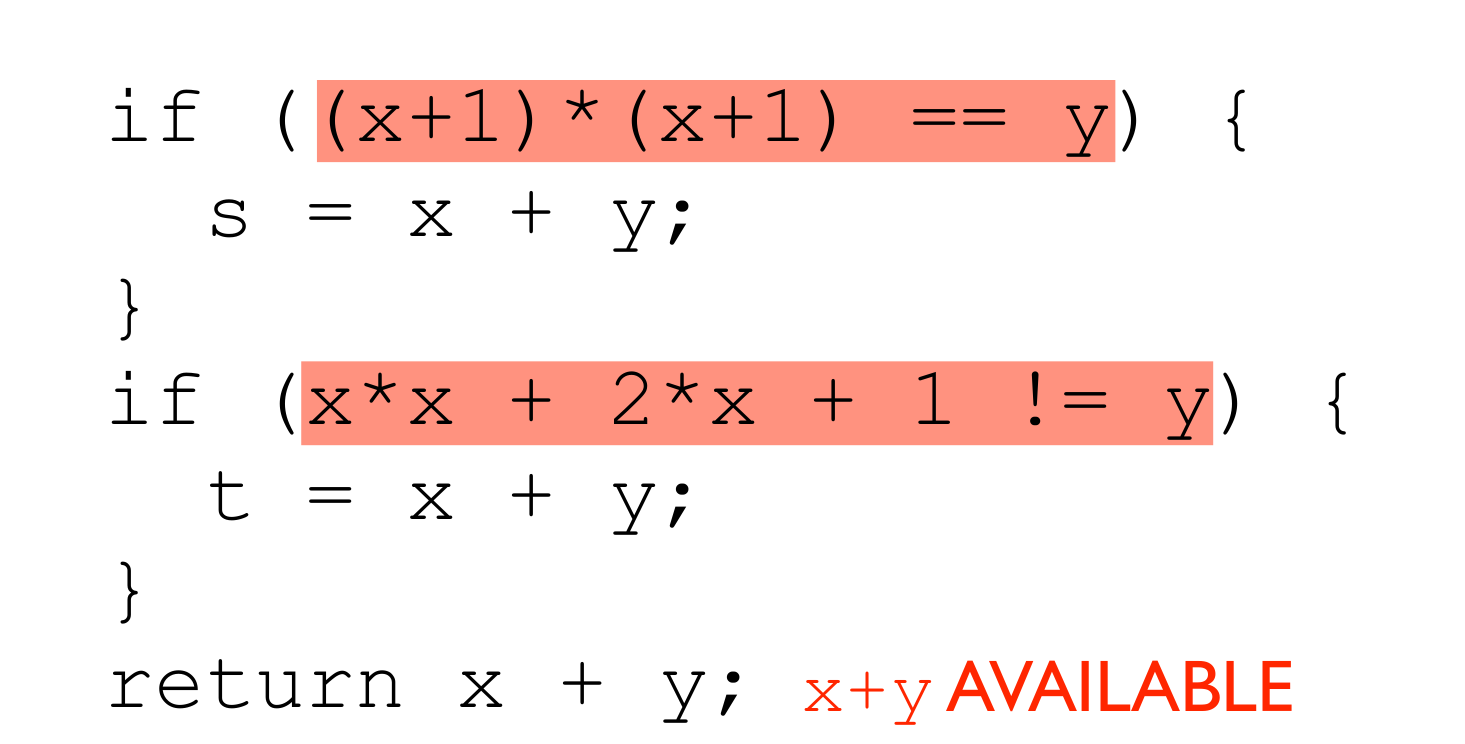
\includegraphics[width=\linewidth]{p4.png}
	\caption{x+y is semantically available}\label{fig:p4}
	\endminipage\hfill
	\minipage{0.4\textwidth}
	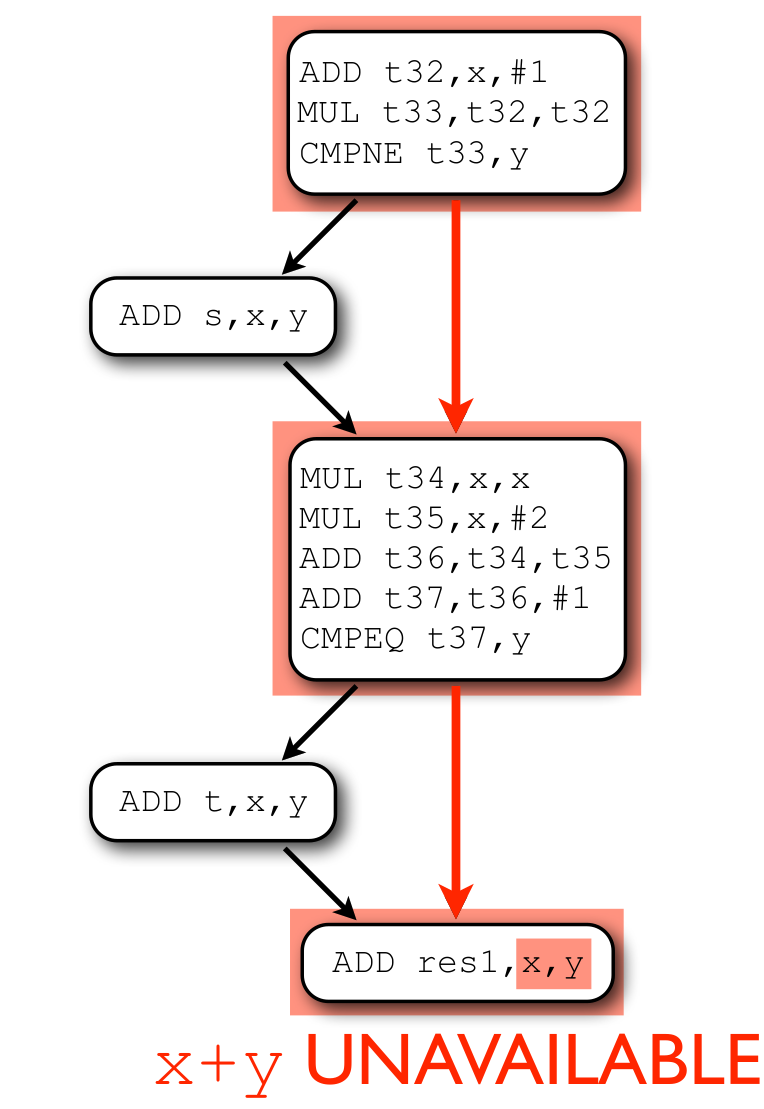
\includegraphics[width=\linewidth]{p3.png}
	\caption{x+y is syntactically unavailable}\label{fig:p3}
	\endminipage
\end{figure}


On the path in red from Figure \ref{fig:p3} through the flowgraph, \(x+y\) is only
computed once, so \(x+y\) is syntactically unavailable at the last instruction.


Whereas with live variable analysis we found safety in assuming that
more variables were live, here we find safety in assuming that fewer
expressions are available. Because if an expression is deemed to be available, we
may do something dangerous (e.g. remove an instruction which recomputes its value).
So sometimes safe means more, but sometimes means less.

\begin{figure}[H]
	\minipage{0.5\textwidth}
	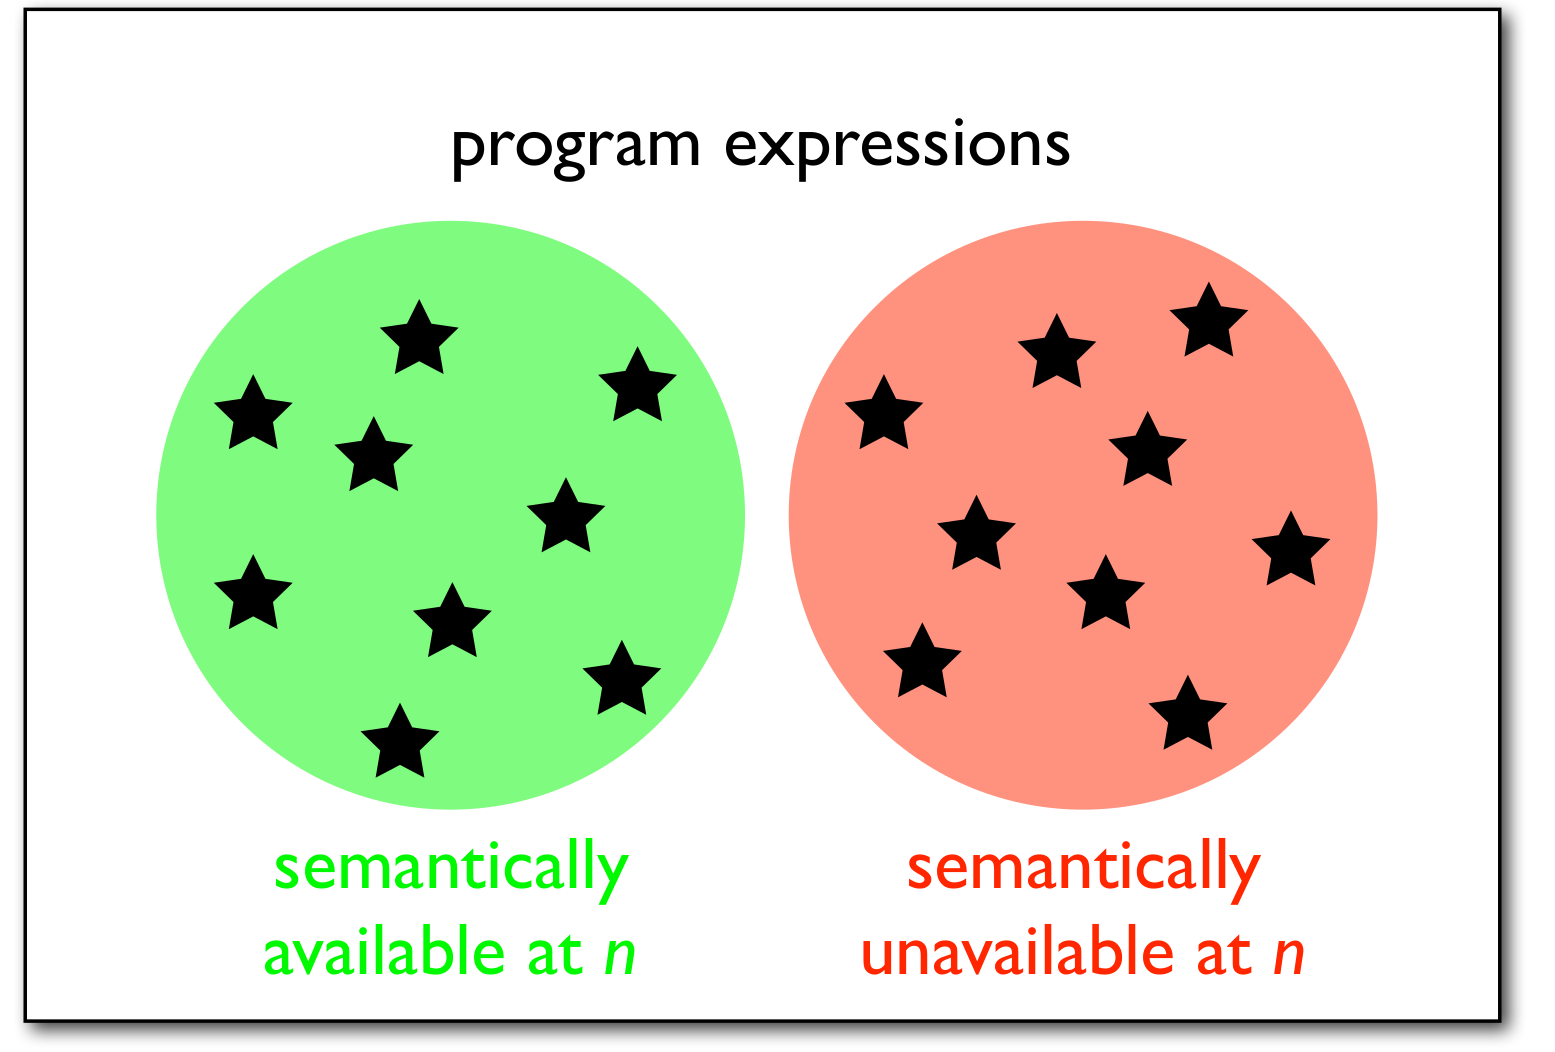
\includegraphics[width=\linewidth]{p5.png}
	\caption{Semantic vs. syntactic}\label{fig:p5}
	\endminipage\hfill
	\minipage{0.5\textwidth}
	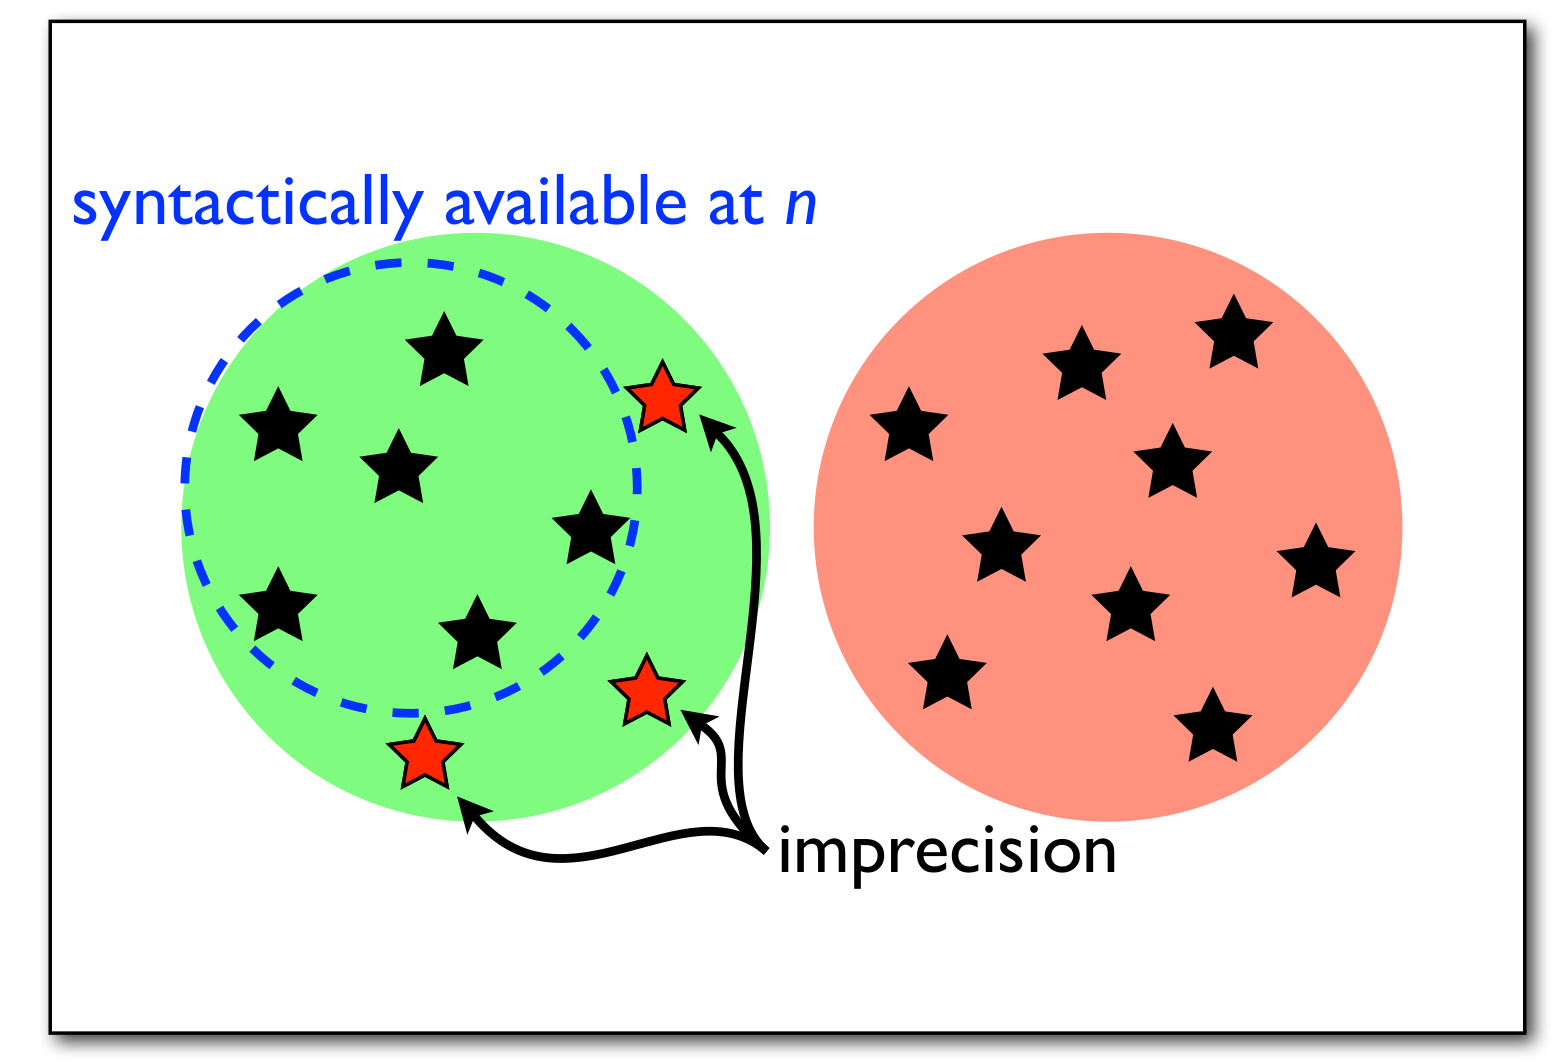
\includegraphics[width=\linewidth]{p6.png}
	\caption{Semantic vs. syntactic}\label{fig:p6}
	\endminipage
\end{figure}


\subsection{Summary}


\begin{center}
	\begin{tabular}{|c|c|}
		\hline Direction                         & Forward                                           \\
		\hline Domain                            & Sets of expressions                                    \\
		\hline Meet operator                     & \( \cap \)                                          \\
		\hline Top(T)                            & Universal Set                                             \\
		\hline Bottom                            & $\phi$                                     \\
		\hline Boundary condition                & $\mathrm{OUT[ENTRY]} = \phi$                          \\
		\hline Initialization for internal nodes & $\mathrm{OUT[B]} = T$                             \\
		\hline Finited escending chain?          & \checkmark                                          \\
		\hline Transfer function                 & $f_b(x) = \mathrm{Gen}_b \cup (x - \mathrm{Kill}_b)$ \\
		\hline Monotone\&Distributive?           & \checkmark                                          \\
		\hline $\mathrm{Kill}_b$ & all E such that block b defines a variable in E \\
    \hline $\mathrm{Gen}_b$ & all E such that block b evaluates E and doesn’t later kill it \\
    \hline
	\end{tabular}
\end{center}
\newpage

\section{Constant Propagation/Folding\cite{Microsof98:online}}


\subsection{Problem Definition }


Given a program, we would like to know for every point in the program (after every
statement), which variables have constant values, and which do not. We say that a
variable has a constant value at a certain point if every execution that reaches that point,
gives that variable the same constant value.


\subsection{Meet Operator}

\begin{figure}[H]
	\centering
	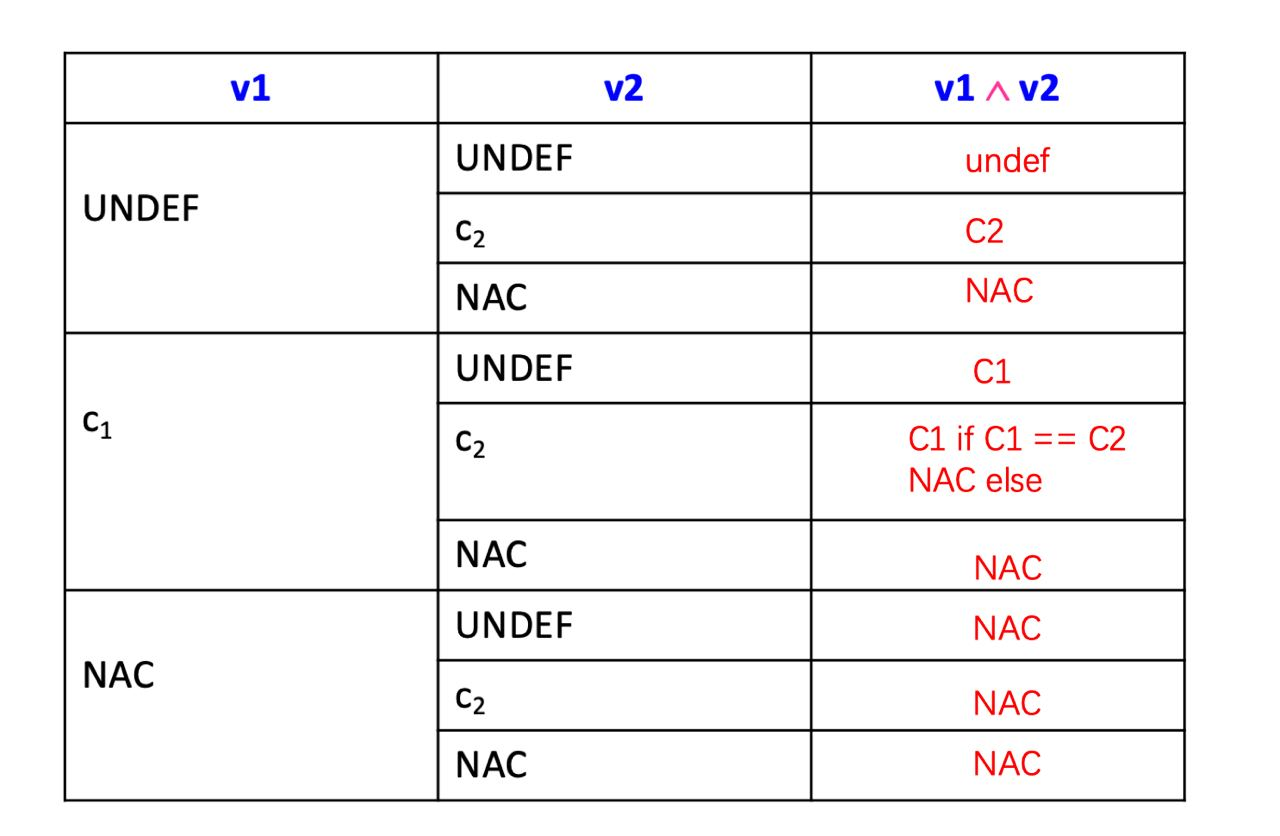
\includegraphics[width=0.6\textwidth]{p219.jpg}
	\caption{Meet operator for Constant Propagation.}
	\label{fig:p219}
\end{figure}


\subsection{Transfer Function}


Let an assignment be of the form $x_3 = x_1 + x_2$, $+$ represents a generic operator.


\begin{figure}[H]
	\centering
	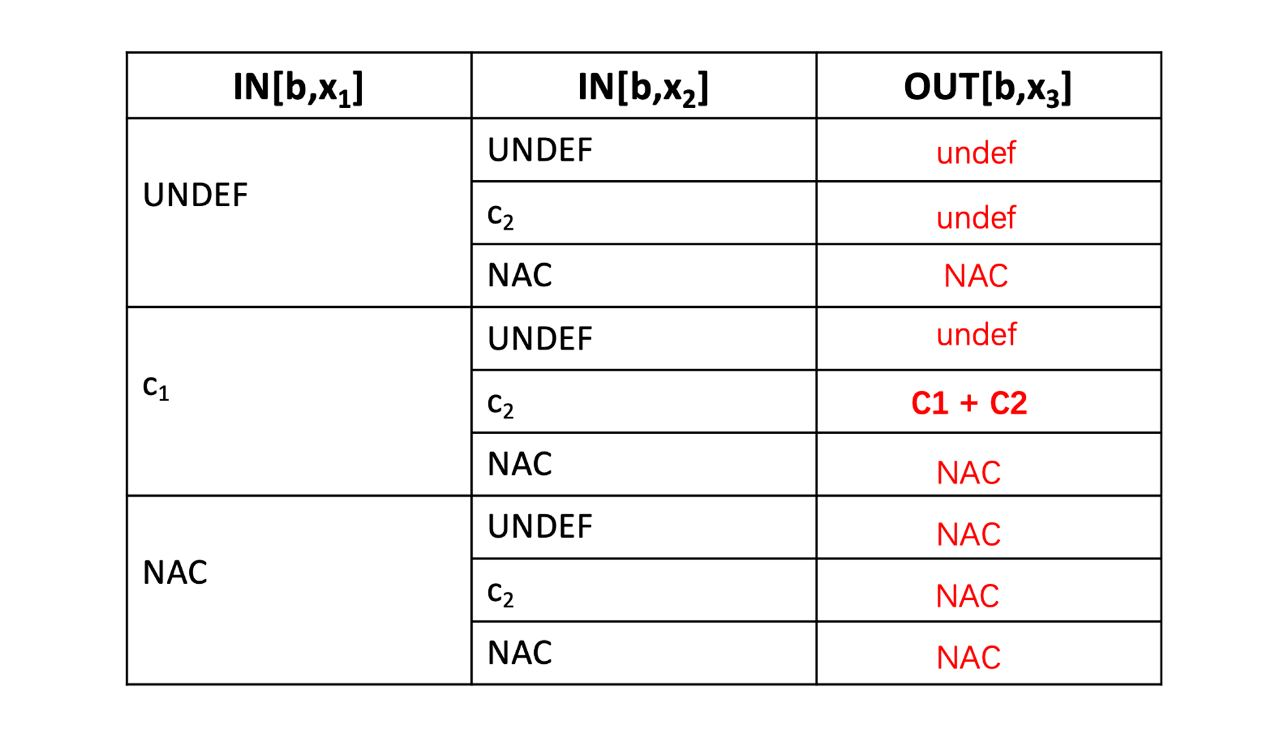
\includegraphics[width=0.6\textwidth]{p220.jpg}
	\caption{Transfer Function.}
	\label{fig:p220}
\end{figure}

\subsection{Summary}
Constant Propogation is not distributive\footnote{See Figure \ref{fig:p221}}.
The semi-lattice is shown in Figure \ref{fig:p222}.



\begin{figure}[H]
	\centering
	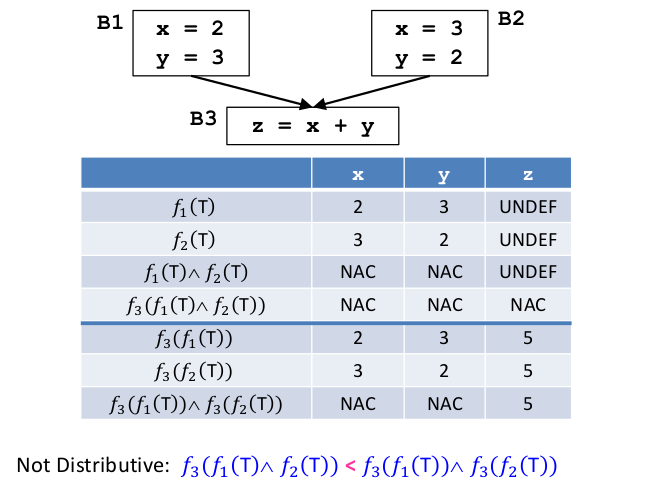
\includegraphics[width=0.6\textwidth]{p222.png}
	\caption{Constant Propogation is not Distributive.}
	\label{fig:p222}
\end{figure}


\begin{figure}[H]
	\centering
	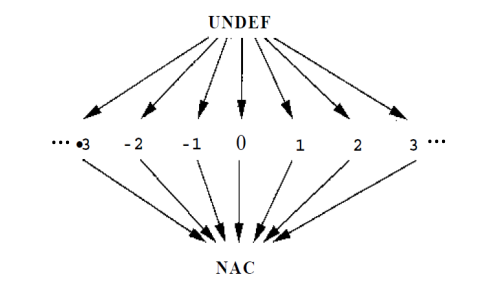
\includegraphics[width=0.6\textwidth]{p221.png}
	\caption{Constant Propogation's Semi-lattice Diagram.}
	\label{fig:p221}
\end{figure}


\begin{center}
	\begin{tabular}{|c|c|}
		\hline Direction                         & Forward                                \\
		\hline Domain                            & Numbers                                \\
		\hline Top(T)                          & $\mathrm{UNDEF}$                       \\
		\hline Bottom                            & $\mathrm{NAC}$                         \\
		\hline Boundary condition                & $\mathrm{OUT[ENTRY]} = \mathrm{UNDEF}$ \\
		\hline Initialization for internal nodes & $\mathrm{OUT[B]} = \mathrm{UNDEF}$     \\
		\hline Finited escending chain?          & \checkmark                             \\
		\hline Monotone ?                        & \checkmark                             \\
		\hline Distributive?                     & \text{\sffamily X}                             \\
		\hline
	\end{tabular}
\end{center}





\section{Foundations of Data Flow Analysis}



Having shown several useful examples of the data-flow abstraction, 
we now study the family of data-flow schemas as a whole, abstractly. 
We shall answer several basic questions about data-flow algorithms formally:

\begin{itemize}

\item Under what circumstances is the iterative algorithm used in data-flow analysis correct?
\item How precise is the solution obtained by the iterative algorithm?
\item Will the iterative algorithm converge?
\item How fast is the convergence?
\end{itemize}


\subsection{Partial Order}\footnote{Based on \url{https://pages.cs.wisc.edu/~horwitz/CS704-NOTES/2.DATAFLOW.html}}

A binary relation R on a set S is called a partial ordering(poset), or partial order if and only if it is:

\begin{itemize}
\item \textbf{Reflexive} \(x \leq x\)
\item \textbf{Antisymmetric} if \(x \leq y\) and \(y \leq x\) then \(x = y\)
\item \textbf{Transitive} if \(x \leq y\) and \(y \leq z\) then \(x \leq z\)
\end{itemize} 



\subsection{Lattices}

A lattice is a poset in which every pair of elements has:

\begin{itemize}
\item a Least Upper Bound (the join of the two elements), and
\item a Greatest Lower Bound (the meet of the two elements).
\end{itemize}    



\subsection{Complete lattices}


A complete lattice is a lattice in which all subsets have a greatest lower bound 
and a least upper bound (the bounds must be in the lattice, but not necessarily 
in the subsets themselves). Note that Every finite lattice (i.e., S is finite) is complete.


\subsection{Monotonic and distributive functions}

A function f: L → L (where L is a lattice) is monotonic iff for all x,y in L: x ⊆ y implies f(x) ⊆ f(y).

A function f: L → L (where L is a lattice) is distributive iff for all x,y in L: f(x meet y) = f(x) meet f(y).

Every distributive function is also monotonic (proving that could be good practice!) but not vice versa. For the GEN/KILL dataflow problems, all dataflow functions are distributive. For constant propagation, all functions are monotonic, but not all functions are distributive.


\subsection{Fixed points}

x is a fixed point of function f iff f(x) = x.

\subsection{Meet Operator}



\newpage

\newpage
\newpage
\newpage

\section{Introduction to Static Single Assignment}

Many dataflow analyses need to find the use-sites of each defined variable or the definition-sites of each variable used in an expression. The \textit{def-use chain} is a data structure that makes this efficient: for each statement in the flow graph, the compiler can keep a list of pointers to all the use sites of variables defined there, and a list of pointers to all definition sites of the variables used there. An improvement on the idea of def-use chains is static single-assignment form, or SSA form, an intermediate representation in which each variable has only one definition in the program text. SSA is very useful for many optimizations such as Loop-Invariant Code Motion and Copy Propagation.

% \subsection{Motivation}

% \begin{itemize}
%     \item The values in reused locations may be provably independent.
%     \item It would be nice if we could traverse directly between related uses and def's
% \end{itemize}

\subsection{Definition-Use and Use-Definition Chains}


\begin{definition}{Use-Definition (UD) Chains}
For a given definition of a variable X, what are all of its uses?

\end{definition}



\begin{definition}{Definition-Use (DU) Chains}
For a given use of a variable X, what are all of the reaching definitions of X?

\end{definition}



Unfortunately, it is expensive to use UD and DU chains, because if we have N defs, and M uses, the space complexity is O(NM). An example is in \ref{fig:p38}


\begin{figure}[htb]
    \centering
    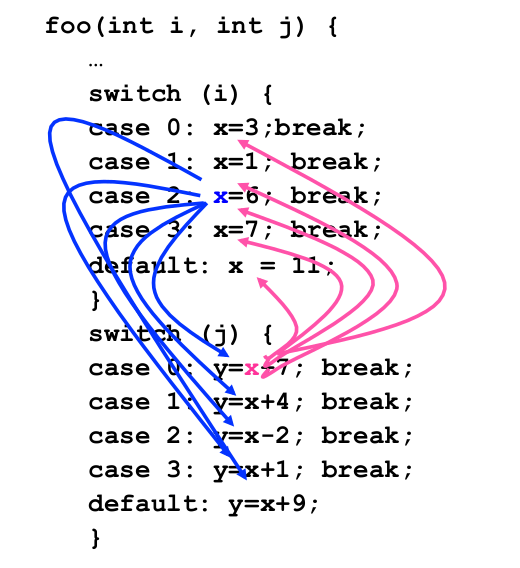
\includegraphics[width=0.3\textwidth]{p38.png}
    \caption{If a variable has N uses and M definitions (which occupy about N + M instructions in a program), it takes space (and time) proportional to N · M to represent def-use chains – a quadratic blowup.}
    \label{fig:p38}
\end{figure}


\subsection{Static Single Assignment(SSA)}

\begin{definition}{Static Single Assignment }
    Static Single Assignment is an IR where every variable is assigned a value at most once in the program text.
\end{definition}








\begin{definition}{the $\Phi$ function}

     $\Phi$ merges multiple definitions along multiple control paths into a single definition.

     At a basic block with p predecessors, there are p arguments to the $\Phi$ functions.

     $$ x_{\text {new }} \leftarrow \Phi\left(\mathbf{x}_1, \mathbf{x}_1, \mathbf{x}_1, \ldots, \mathbf{x}_{\mathrm{p}}\right)
     $$
\end{definition}

\subsubsection{Why SSA is useful?}

\textbf{ \large \textit{Useful for Dataflow Analysis}} Dataflow analysis and optimization algorithms can be made simpler when each variable has only one definition.

\textbf{ \large \textit{Less space and time complexity}} If a variable has N uses and M definitions (which occupy about N + M instructions in a program), it takes space (and time) proportional to N · M to represent def-use chains – a quadratic blowup. For almost all realistic programs, the size of the SSA form is linear in the size of the original program.


\textbf{ \large \textit{Simplify some algorithms}} Uses and defs of variables in SSA form relate in a useful way to the dominator structure of the control-flow graph, which simplifies algorithms such as interference-graph construction.


\textbf{ \large \textit{Eliminate needless relationship}} Unrelated uses of the same variable in the source program become different variables in SSA form, eliminating needless relationships shown in \ref{exp:1}.

\begin{lstlisting}[label={exp:1},caption={An example}]

for i <- 1 to N do A[i] <- 0
for i <- 1 to M do s <- s + B[i]

\end{lstlisting}


\subsection{How to represent SSA?}

In straight-line code, such as within a basic block, it is easy to see that each instruction can define a fresh new variable instead of redefining an old one shown in \ref{fig:p42-43}


\begin{figure}[htb]
     \centering
     \begin{subfigure}{0.2\textwidth}
     \centering
         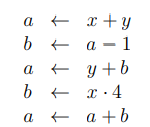
\includegraphics[width=\textwidth]{p42.png}
         \caption{A straight-line program.}
         \label{fig:p42}
     \end{subfigure}
     \begin{subfigure}{0.25\textwidth}
     \centering
         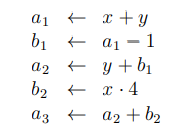
\includegraphics[width=\textwidth]{p43.png}
         \caption{The program in single-assignment form.}
         \label{fig:p43}
     \end{subfigure}
        \caption{SSA for straight-line code}
        \label{fig:p42-43}
\end{figure}


But when two control-flow paths merge together, it is not obvious how to have only one assignment for each variable. To solve this problem we introduce a notational fiction, called a $\Phi$ function. Figure \ref{fig:p44} shows that we can combine a1 (defined in block 1) and a2 (defined in block 3) using the function $a3 \leftarrow \Phi(a1, a2)$.


\begin{figure}[htb]
    \centering
    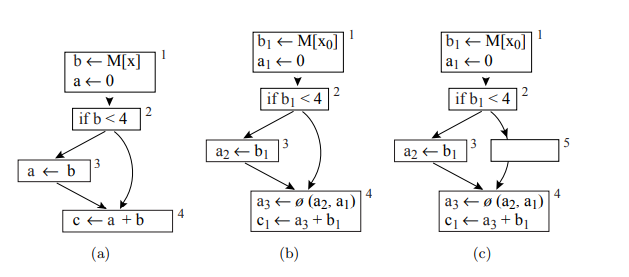
\includegraphics[width=0.8\textwidth]{p44.png}
    \caption{(a) A program with a control-flow join; (b) the program transformed to single-assignment form; (c) edge-split SSA form.}
    \label{fig:p44}
\end{figure}


unlike ordinary mathematical functions, $\Phi$(a1, a2) yields a1 if control reaches block 4 along the edge $2 \rightarrow 4$, and yields a2 if control comes in on edge $3 \rightarrow 4$.


\subsubsection{How does the $\phi$-function know which edge was taken?}


If we must execute the program, or translate it to executable form, we can “implement” the $\Phi$-function using a move instruction on each incoming edge as shown in Figure \ref{fig:p39-40}. However, in many cases, we simply need the connection of uses to definitions and don’t need to “execute” the $\Phi$-functions during optimization. In these cases, we can ignore the question of which value to produce.

\begin{figure}[htb]
     \centering
     \begin{subfigure}{0.3\textwidth}
     \centering
         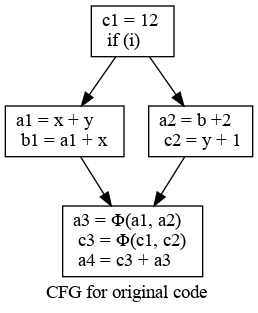
\includegraphics[width=\textwidth]{p39.png}
         \caption{Original code}
         \label{fig:p39}
     \end{subfigure}
     \begin{subfigure}{0.3\textwidth}
     \centering
         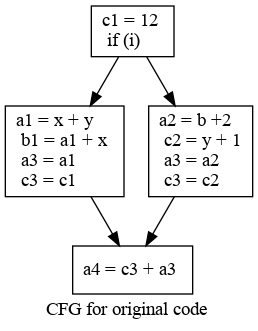
\includegraphics[width=\textwidth]{p40.png}
         \caption{Code after moving instruction.}
         \label{fig:p40}
     \end{subfigure}
        \caption{Implementing $\Phi$-function}
        \label{fig:p39-40}
\end{figure}




\subsection{Converting to SSA form}

The algorithm for converting a program to SSA form is roughly as follows:

\begin{itemize}
    \item 1. adds $\Phi$ functions for the variables, and then
    \item 2. renames all the definitions and uses of variables using subscripts.
\end{itemize}




\subsubsection{Trivial SSA}

Trivial SSA form is based on a simple observation: $\Phi$ functions are only needed for variables that are "live" after the $\Phi$ function.

\begin{itemize}
    \item Each assignment generates a fresh variable.
    \item At each join point insert $\Phi$ for all live variables.
\end{itemize}


Trivial SSA will generate some useless $\Phi$ functions. An example is shown in Figure \ref{fig:p41} So a $\Phi$-function is not needed for every variable at each point.

\begin{figure}[htb]
    \centering
    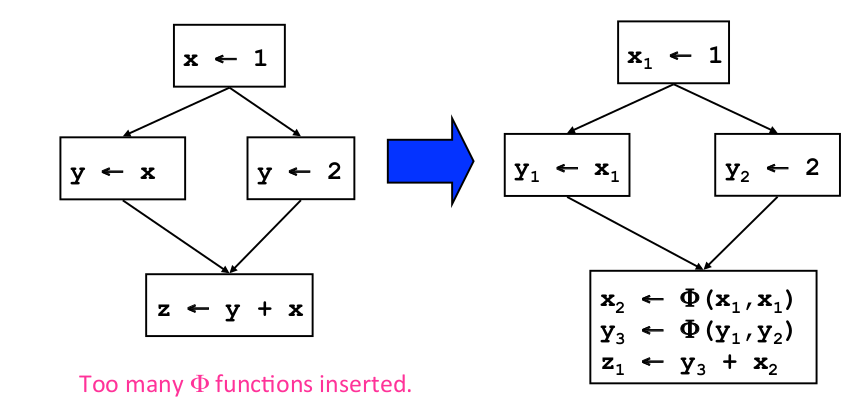
\includegraphics[width=0.5\textwidth]{p41.png}
    \caption{$x2 \leftarrow \Phi(x1,x1)$ is useless because x2 is equal to x1.}
    \label{fig:p41}

\end{figure}



\subsubsection{Minimal SSA}
Minimal SSA is an updated version compared to trivial SSA.

\begin{itemize}
    \item Each assignment generates a fresh variable.
    \item At each join point insert $\Phi$ for all live variables with multiple outstanding defs. 
\end{itemize}

\subsubsection{Path-convergence criterion}

There should be a $\Phi$-function for variable a at node z of the flow graph
exactly when all of the following are true:

\begin{itemize}
    \item 1. There is a block x containing a definition of a,
    \item 2. There is a block y (with $y \neq x$) containing a definition of a,
    \item 3. There is a nonempty path $P_{xz}$ of edges from x to z,
    \item 4. There is a nonempty path $P_{yz}$ of edges from y to z,
    \item 5. Paths $P_{xz}$ and $P_{yz}$ do not have any node in common other than z, and
    \item 6. The node z does not appear within both $P_{xz}$ and $P_{yz}$ prior to the
end, though it may appear in one or the other.
\end{itemize}


We consider the start node to contain an implicit definition of every variable, either because the variable may be a formal parameter or to represent the notion of a 
$\leftarrow$ uninitialized without special cases. A $\Phi$-function itself counts as a definition of a, so the path-convergence criterion must be considered as a set of equations to be satisfied. As usual, we can solve them by iteration as shown in \ref{alg:Iterated path-convergence criterion}.


\begin{algorithm}
\caption{Iterated path-convergence criterion}\label{alg:Iterated path-convergence criterion}
\begin{algorithmic}

\While{there are nodes $x, y, z$ satisfying conditions 1–5
and \\ $z$ does not contain a $\Phi$-function for a}
\State  insert a $\leftarrow$ $\Phi$(a, a, . . . , a) at node Z
\EndWhile
\end{algorithmic}
\end{algorithm}

\subsubsection{Dominance property of SSA form}

The iterated path-convergence algorithm for placing $\Phi$-functions is not practical, since it would be very costly to examine every triple of nodes x, y, z, and every path leading from x and y.  A much more efficient algorithm using the dominator tree of the flow graph as shown in Figure \ref{fig:p45}.


\begin{figure}[H]
    \centering
    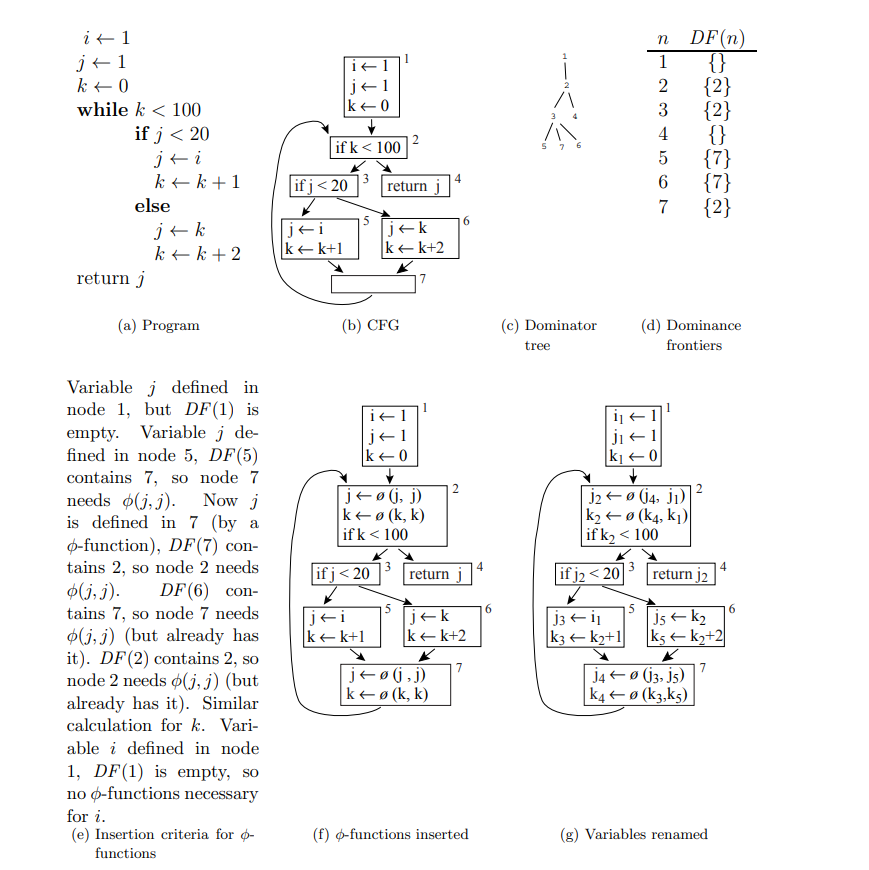
\includegraphics[width=\textwidth]{p45.png}
    \caption{ Conversion of a program to static single-assignment form. Node 7 is a postbody node, inserted to make sure there is only one loop edge; such nodes are not strictly necessary but are sometimes helpful.}
    \label{fig:p45}

\end{figure}


\begin{definition}{Strictly dominance}
    x strictly dominates w (x sdom w) iff impossible to reach w without passing through x first.
\end{definition}

\begin{definition}{Dominance}
    x  dominates w (x dom w) iff x sdom w or x = w.
$$
\operatorname{Dom}(n)= \begin{cases}\{n\} & \text { if } n=n_0 \\ \{n\} \cup\left(\bigcap_{p \in \operatorname{preds}(n)} \operatorname{Dom}(p)\right) & \text { if } n \neq n_0\end{cases}
$$
\end{definition}

\begin{definition}{Dominance tree}
    x sdom w iff x is a proper ancestor of w.  

\end{definition}

\begin{definition}{Dominance Frontier}


The dominance frontier of a node x is the set of all nodes w such that
x dominates a predecessor of w, but does not strictly dominate w.

$$
F(x)=  \{w | \texttt{x  dom pred(w) AND   !(x  sdom  w) } \}
$$
\end{definition}





An essential property of static single assignment form is that definitions dominate uses; more specifically,
\begin{itemize}
    \item  If x is the ith argument of a $\Phi$-function in block n, then the definition of x dominates the ith predecessor of n.
    \item  If x is used in a non-$\Phi$ statement in block n, then the definition of x dominates n
\end{itemize}

\begin{note}{Dominance Property of SSA	}
  In SSA,

  \begin{itemize}
      \item If x i is used in $x \leftarrow \Phi (..., x_i , ...)$, then $BB(x_i )$ dominates ith predecessor of $BB(\Phi)$
      \item If x is used in $y \leftarrow ...x...$,then BB(x) dominates BB(y)
  \end{itemize}
\end{note}


\textbf{ \large \textit{Dominance frontier criterion.}} Whenever node x contains a definition of some variable a, then any node z in the dominance frontier of x needs a $\Phi$-function for a.


\textbf{ \large \textit{Iterated dominance frontier.}} Since a $\Phi$-function itself is a kind of definition, we must iterate the dominance-frontier criterion until there are no nodes that need $\Phi$-functions.


\textbf{ \large \textit{Theorem.}} The iterated dominance frontier criterion and the iterated path convergence criterion specify exactly the same set of nodes at which to put $\Phi$-functions

\begin{figure}[htb]
    \centering
    \includegraphics[width=\textwidth]{p46.png}
    \caption{Node 5 dominates all the nodes in the grey area. (a) Dominance frontier of node 5 includes the nodes (4, 5, 12, 13) that are targets of edges crossing from the region dominated by 5 (grey area including node 5) to the region not strictly dominated by 5 (white area including node 5). (b) Any node in the dominance frontier of n is also a point of convergence of nonintersecting paths, one from n and one from the root node. (c) Another example of converging paths $P_{1,5}$ and $P_{5,5}$.}
    \label{fig:p46}

\end{figure}


\begin{proof}{Proof}
The sketch of a proof that shows if w is in the dominance frontier of a definition, then it must be a point of convergence.

Suppose there is a definition of variable a at some node n (such as node 5 in Figure  \ref{fig:p46}b), and node w (such as node 12 in Figure  \ref{fig:p46}b) is in the dominance frontier of n. The root node implicitly contains a definition of every variable, including a. There is a path $P_{rw}$ from the root node (node 1 in Figure \ref{fig:p46}) to w that does not go through n or through any node that n dominates; and there is a path $P_{nw}$ from n to w that goes only through dominated nodes. These paths have w as their first point of convergence.
\end{proof}


\subsection{Computing the dominance frontier}

To insert all the necessary $\Phi$-functions, for every node n in the flow graph we need DF[n], its dominance frontier. Given the dominator tree, we can efficiently compute the dominance frontiers of all the nodes of the flow graph in one pass. We define two auxiliary sets

\begin{itemize}
    \item $DF_{local}[n]$ The successors of n that are not strictly dominated by n;
    \item $DF_{up}[n]$ Nodes in the dominance frontier of n that are not dominated by n’s immediate dominator.
\end{itemize}

The dominance frontier of n can be computed from $DF_{local}[n]$  and $DF_{up}[n]$ 


$$
D F[n]=D F_{\text {local }}[n] \quad \cup \quad \bigcup_{c \in \text { children }[n]} D F_{\text {up }}[c]
$$

where children[n] are the nodes whose immediate dominator (idom) is n.


To compute $DF_{local}[n]$ \ref{alg:computeDF} more easily (using immediate dominators instead of dominators), we use the following theorem: $DF_{local}[n]$ = the set of those successors of n whose immediate dominator is not n. The following computeDF function should be called on the root of the dominator tree (the start node of the flow graph). It walks the tree computing DF[n] for every node n: it computes $DF_{local}[n]$ by examining the successors of n, then combines $DF_{local}[n]$ and (for each child c) $DF_{up}[n]$.a

\begin{algorithm}
\caption{computeDF}\label{alg:computeDF}
\begin{algorithmic}

\State $S \gets \{\}$
\For{each node y in succ[n]} \Comment{This loop computes $DF_{local}[n]$}
\If {idom(y) $\neq$ n}
\State $S\leftarrow S \cup \{y\}$
\EndIf 
\EndFor

\For{each child c of n in the dominator tree} 
\State computeDF[c]
\For{each element w of DF[c]} \Comment{This loop computes $DF_{up}[n]$}
\If {n does not dominate w}
\State $S\leftarrow S \cup \{w\}$
\EndIf 
\EndFor
\EndFor
\end{algorithmic}
\end{algorithm}

This algorithm is quite efficient. It does work proportional to the size (number of edges) of the original graph, plus the size of the dominance frontiers it computes. Although there are pathological graphs in which most of the nodes have very large dominance frontiers, in most cases the total size of all the DFs is approximately linear in the size of the graph, so this algorithm runs in “practically” linear time.




\subsection{Inserting $\Phi$-functions}

Starting with a program not in SSA form, we need to insert just enough $\Phi$-functions to satisfy the iterated dominance frontier criterion. To avoid re-examining nodes where no $\Phi$-function has been inserted, we use a work-list algorithm.

\begin{algorithm}
\caption{Place-$\Phi$-Functions}\label{alg:Place-Phi-Functions}
\begin{algorithmic}
\For{each node n}
\For{each variable a in $A_{orig}[n]$}
\State defsites[a] $\gets$ defsites[a] $\cup \{n\}$
\EndFor
\EndFor


\For{each variable a}
\State W $\gets$ defsites[a]
\While{ W not empty}
\State{remove some node n from W}
\For{each y in DF[n]}
\If{y $\not\in$ $A_{\Phi}[a]$}
\State{insert the statement a $\gets$ $\Phi$(a, a, . . . , a) at the top of block y, where the $\Phi$-function has as many arguments as y has predecessors}
\State{$A_{\Phi}[a] \gets A_{\Phi}[a] \cup \{ y\}$}
\If{a $\not\in$ $A_{orig}[y]$}
\State{$W \gets W \cup \{y \}$}
\EndIf

\EndIf
\EndFor
\EndWhile
\EndFor

\end{algorithmic}
\end{algorithm}


Algorithm\ref{alg:Place-Phi-Functions} starts with a set V of variables, a graph G of controlflow nodes – each node is a basic block of statements – and for each node n a set $A_{orig}$[n] of variables defined in node n. The algorithm
computes $A_{\Phi}[a]$, the set of nodes that must have $\Phi$-functions for variable
a. Sometimes a node may contain both an ordinary definition and a
$\Phi$-function for the same variable; for example, in Figure \ref{fig:p46}b, a $\in$ $A_{orig}[2]$
and 2 $\in$ $A_{\Phi}[a]$.


This algorithm does a constant amount of work (a) for each node and edge in the control-flow graph, (b) for each statement in the program, (c) for each element of every dominance frontier, and (d) for each inserted $\Phi$-function. For a program of size N, the amounts a and b are proportional to N, c is usually approximately linear in N. The number of inserted $\Phi$-functions (d) could be $N^2$ in the worst case, but empirical measurement has shown that it is usually proportional to N. So in practice, Algorithm \ref{alg:Place-Phi-Functions} runs in approximately linear time.


\subsection{Renaming the variables}

After the $\Phi$-functions are placed, we can walk the dominator tree, renaming the different definitions (including $\Phi$-functions) of variable a to a1, a2, a3 and so on. Rename each use of a to use the closest definition d of a that is above a in the dominator tree. Algorithm  renames all uses and definitions of variables, after the $\Phi$-functions have been inserted by Algorithm \ref{alg:Renaming variables}. In traversing the dominator tree, the algorithm “remembers” for each variable the most recently defined version of each variable, on a separate stack for each variable. Although the algorithm follows the structure of the dominator tree – not the flow graph – at each node in the tree it examines all outgoing flow edges, to see if there are any $\Phi$-functions whose operands need to be properly numbered.



\begin{algorithm}
\caption{Renaming variables.}\label{alg:Renaming variables}
\begin{algorithmic}
\State Initialization:

\For{each variable a}
\State{Count[a] $\gets$ 0}
\State{Stack[a] $\gets$ empty}
\State{push 0 onto Stack[a]}
\EndFor

\State{Rename(n) }
\For{each statement S in block n}
\If{S is not a $\Phi$-function}
\For{each use of some variable x in S}
\State{i $\gets$ top(Stack[x])}
\State{replace the use of x with $x_i$ in S}
\EndFor
\EndIf
\For{each definition of some variable a in S}

\State Count[a] $\gets$ Count[a]+1
\State i $\gets$ Count[a]
\State push i onto Stack[a]
\State replace definition of a with definition of $a_i$ in S
\EndFor
\EndFor

\For{each successor Y of block n,}
\State Suppose n is the jth predecessor of Y
\For{each $\Phi$-function in Y}
\State suppose the jth operand of the $\Phi$-function is a
\State i $\gets$ top(Stack[a])
\State replace the jth operand with $a_i$

\EndFor
\EndFor
\For{each child X of n}
\State Rename(X)
\EndFor
\For{each definition of some variable a in the original S}
\State pop Stack[a]
\EndFor
\end{algorithmic}
\end{algorithm}




\subsection{Edge Splitting}

Some analyses and transformations including reverse transformation from SSA back into a normal form are simpler if there is never a controlflow edge that leads from a node with multiple successors to a node with multiple predecessors. To give the graph this unique successor or predecessor property, we perform the following transformation: For each control-flow edge a $\gets$ b such that a has more than one successor and b has more than one predecessor, we create a new, empty controlflow node z, and replace the a $\gets$ b edge with an a $\gets$ z edge and a z $\gets$ b edge.

An SSA graph with this property is in edge-split SSA form. Figure \ref{fig:p44} illustrates edge splitting. Edge splitting may be done before or after insertion of $\Phi$-functions.
\newpage

\section{SSA-Style optimizations}

\subsection{Constant Propagation}
\begin{note}{notes}
\begin{itemize}
    \item If  v $\gets$ c , replace all uses of v with c 
    \item If  v $\gets$  $\Phi$ (c,c,c)  (each input is the same constant), replace all uses of v with c
\end{itemize}
\end{note}


\begin{algorithm}
\caption{SSA-CP}\label{alg:SSA-CP}
\begin{algorithmic}
\State{W $\gets$ ist of all defs}
\While{!W.isEmpty}

\State{Stmt S $\gets$ W.removeOne}
\If{(S has form v $\gets$ c) or
(S has form v $\gets$ $\Phi$(c,...,c))}
\State delete S
\For{each stmt U that uses v}
\State {replace v with c in U}
\State {W.add(U)}
\EndFor
\EndIf
\EndWhile

\end{algorithmic}
\end{algorithm}

\subsection{Conditional Constant Propagation }

Wegman and Zadeck's Sparse Conditional Constant (SCC) algorithm was used to find constant expressions, constant conditions, and unreachable code [WZ91]. The output of the SCC algorithm is an association of variables to one of $\lbrace \bot, c, \top \rbrace$, where $\bot$ marks a variable that can hold different values at different times, and $\top$ means the variable is not executed. In addition, every flow-graph node (corresponding to a quadruple) is marked as executable or non-executable. We then walk the flow-graph, eliminating dead-code (quadruples marked non-executable), replacing constant variables with their values, and changing constant conditional branches to goto statements.

\begin{note}{notes}
\begin{itemize}
    \item Assume all blocks unexecuted until proven otherwise
    \item Assume all variables are not executed (only with proof of assignment of a non-constant value do we assume not constant)
\end{itemize}
\end{note}

\subsubsection{Example}

\begin{figure}[H]
    \centering
     \includegraphics[width=\textwidth]{p47.pdf}
         \caption{Original code. The black block is marked as unexecuted}
         \label{fig:p47}

\end{figure}




\begin{figure}[H]
    \centering
     \includegraphics[width=0.8\textwidth]{p48.pdf}
         \caption{The read block is marked as executed. After walking the first two blocks, the value is shown above.}
         \label{fig:p48}

\end{figure}



\begin{figure}[H]
    \centering
     \includegraphics[width=0.8\textwidth]{p49.pdf}
         \caption{After walking 5 blocks.}
         \label{fig:p49}

\end{figure}



\begin{figure}[H]
    \centering
     \includegraphics[width=0.8\textwidth]{p50.pdf}
         \caption{Now k2 is $\bot$, so the \texttt{return j2} is reachable.}
         \label{fig:p50}

\end{figure}



\begin{figure}[H]
    \centering
     \includegraphics[width=0.5\textwidth]{p51.pdf}
         \caption{Code after applied SCC.}
         \label{fig:p51}

\end{figure}


% \begin{figure}[!b]
%      \centering
%      \begin{subfigure}{0.45\textwidth}
%      \centering
%          \includegraphics[width=\textwidth]{p47.pdf}
%          \caption{Original code}
%          \label{fig:p47}
%      \end{subfigure}
%      \begin{subfigure}{0.6\textwidth}
%      \centering
%          \includegraphics[width=\textwidth]{p48.pdf}
%          \caption{Code after moving instruction.}
%          \label{fig:p48}
%      \end{subfigure}
%           \begin{subfigure}{0.6\textwidth}
%      \centering
%          \includegraphics[width=\textwidth]{p49.pdf}
%          \caption{Code after moving instruction.}
%          \label{fig:p49}
%      \end{subfigure}
%           \begin{subfigure}{0.6\textwidth}
%      \centering
%          \includegraphics[width=\textwidth]{p50.pdf}
%          \caption{Code after moving instruction.}
%          \label{fig:p50}
%      \end{subfigure}
%           \begin{subfigure}{0.6\textwidth}
%      \centering
%          \includegraphics[width=\textwidth]{p51.pdf}
%          \caption{Code after moving instruction.}
%          \label{fig:p51}
%      \end{subfigure}
%         \caption{Implementing $\Phi$-function}
%         \label{fig:p47-51}
% \end{figure}




\subsection{Copy Propogation}

\begin{note}{notes}
\begin{itemize}
    \item  delete x $\gets \Phi$ (y,y,y) and replace all x with y
    \item delete x $\gets$ y and replace all x with y
\end{itemize}
\end{note}







\newpage

\section{The LLVM project}

LLVM is an open-source framework providing a modern collection of modular and reusable
compiler and toolchain technologies [20]. The project stemmed from the work of Chris
Lattner, who first implemented core elements of LLVM to support the research of his
master thesis in 2002 [26]. One of the key strengths of LLVM is that it faces active
development from an expert community of contributors, and is widely used across the
industry and academia alike [11]. The project received the ACM Software System Award
in 2012 [4] as an acknowledgement of its contribution to compiler research and implementation.

LLVM officially acknowledges more than 10 main sub-projects [20], which range in diversity from a debugger [9] to a symbolic execution tool [8]. In addition to these, the official
website presents a long list of miscellaneous projects that are based on components of
the LLVM infrastructure [19].

All projects which are part of the LLVM ecosystem are built upon the core libraries, which
are arguably the centrepiece of LLVM. They host the source- and target-independent
optimizer (Section 3.3), the implementation of the LLVM intermediate representation
(Section 3.2), and a suite of command-line tools useful for code manipulation (Section 3.4).
The core libraries also implement various back-end passes that translate IR to machine
code for different platforms (x86, PowerPC, Nvidia GPUs).
For building a complete compiler for a source language, the LLVM core libraries readily
provide the optimizing pass and code generation for common architectures, the frontend being the only missing component. Clang is by far the most prominent front-end
implemented in LLVM [5], and it targets the family of C languages (C/C++ and Objective-C/C++). Coupled with the core libraries, Clang is a powerful compiler
producing high-performance code, and positions itself as a direct competitor to both gcc
and the Intel compiler.


\newpage

\section{Loop Invariant Computation and Code Motion}


Loop-Invarian Code Motion (LICM) recognizes computations within a loop that produce the same result each time the loop is executed. 
These computations are called loop-invariant code and can be moved outside the loop body without changing the program semantics. 
The positive effects of LICM are:
\begin{itemize}
\item The shifted loop invariants exhibit a reduced execution frequency.
\item The transformation may shorten variable live ranges leading to a decreased register pressure. This circumstance may in turn reduce the number of required spill code instructions.
\item Moving code outside a loop reduces the loop's size which may be beneficial for the I-cache behavior since more loop code can reside in the cache.
\end{itemize}

Besides these positive effects on the code, LICM may also degrade performance. This is mainly due to two reasons. First, the newly created variables to store the loop-invariant results outside the loop, may increase the register pressure in the loops since their live ranges span across the entire loop nest. As a result, possibly additional spill code is generated. 
Second, LICM might lengthen other paths of the control flow graph. This situation can be observed if the invariants are moved from a less executed to a more frequently executed path, e.g., moving instructions above a loop's zero-trip test.


\subsection{Finding natrual loops}

Not every cicle is a loop in CFG. From a intuitive perspective, a loop must has a single entry and edges must from at least one circle.   

\begin{definition}{Back Edge}
    A back edge is an arc t$\rightarrow$h whose
head h dominates its tail t
\end{definition}

\begin{definition}{Natural Loop}
    The natural loop of a back edge t$\rightarrow$h
    is the smallest set of nodes that
    includes t and h, and has
    no predecessors outside the set,
    except for the predecessors of the header h.
\end{definition}

\begin{definition}{Reducible}
A flow graph is reducible if every retreating edge in any DFST (Deep-First Spanning Tree) for that flow graph is a back edge.
\end{definition}



\paragraph{Testing reducibility} Take any DFST for the flow graph, remove the back edges, and check that the result is acyclic.

\begin{figure}[H]
    \centering
    \includegraphics[width=0.5\textwidth]{DFST.png}
    \caption{Example: Nonreducible Graph }
    \label{fig:DFST}
\end{figure}

\subsection{Algorithm to Find Natural Loops}

\subsubsection{Step 1. Finding Dominators}

We can formulate this as Data Flow Analysis problem. Since Node d dominates node n in a graph (d dom n)
if every path from the start node to n goes through d. So if d dom n iff iff d dom p for all pred p of n.
\begin{center}
 \begin{tabular}{|c|c|}
\hline Direction & Forward\\
\hline Values & Basic Blocks\\
\hline Meet operator & \( \cap \)\\
\hline Top(T) & Universal Set\\
\hline Bottom & $\phi$\\
\hline Boundary condition for entry node & $\phi$ \\  
\hline Initialization for internal nodes & \(\mathrm{T}\) \\
\hline Finited escending chain? &\checkmark  \\
\hline Transferfunction  & $\text { OUT }[\mathbf{b}]=\{\mathbf{b}\} \cup\left(\cap_{\{\boldsymbol{p}=\boldsymbol{p r e d}(\boldsymbol{b})\}} \text { OUT }[\mathbf{p}]\right)$ \\
\hline Monotone\&Distributive?  & \checkmark \\
\hline
\end{tabular}  
\end{center}


With rPostorder, most flow graphs (reducible flow graphs) converge in 1 pass. 


\begin{figure}[H]
    \centering
    \begin{subfigure}{0.3\textwidth}
    \centering
        \includegraphics[width=\textwidth]{p61.png}
        \caption{CFG.}
        \label{fig:p61}
    \end{subfigure}
    \begin{subfigure}{0.3\textwidth}
    \centering
        \includegraphics[width=\textwidth]{p62.png}
        \caption{Dominance Tree of the corresponding CFG.}
        \label{fig:p62}
    \end{subfigure}
    
    \caption{An example of Dominance tree.}
       \label{fig:p51-58}
\end{figure}



\subsubsection{Step 2. Finding Back Edges}

\paragraph{Depth-first spanning tree}
Edges traversed in a depth-first search of the flow graph form a depth-first spanning tree. We categorize edges in CFG as follows:
\begin{itemize}
    \item Forward edges (node to proper descendant).
    \item Retreating edges (node to ancestor).
    \item Cross edges (between two nodes, neither of which is an ancestor of the other.)
\end{itemize}

This is something difficult to understand. Let's make it simpler. We can number each node when we visit it. So each edge should be satisfied the following property:


\begin{center}
\begin{tabular}{|c|c|}
\hline Forward/Advancing edges  \( n_1 \rightarrow n_2\) & num($n_1$) $<$ num($n_2$) and  $n_1$ is ancestor of  $n_2$\\
\hline Cross edges  \( n_1 \rightarrow n_2\)& num($n_1$) $>$ num($n_2$) and neither  $n_1$ is ancestor of  $n_2$ nor $n_2$ is ancestor of  $n_1$ \\
\hline Retreating edges  \( n_1 \rightarrow n_2\) & num($n_1$) $>$ num($n_2$) and  $n_2$ is ancestor of  $n_1$\\
\hline
\end{tabular}  
\end{center}





Of these edges, only retreating edges go from high to low in DF order.



\paragraph{Algorithm}

\begin{itemize}
    \item Perform a depth first search
    \item For each retreating edge \(t \rightarrow h\), check if h is in t$^\prime$s dominator list
\end{itemize}


\begin{figure}[H]
    \centering
    \begin{subfigure}{0.3\textwidth}
    \centering
        \includegraphics[width=\textwidth]{p61.png}
        \caption{CFG.}
        \label{fig:p61}
    \end{subfigure}
    \begin{subfigure}{0.3\textwidth}
    \centering
        \includegraphics[width=\textwidth]{p62.png}
        \caption{Dominance Tree of the corresponding CFG.}
        \label{fig:p62}
    \end{subfigure}
    \begin{subfigure}{0.3\textwidth}
        \centering
            \includegraphics[width=\textwidth]{p63.jpg}
            \caption{{\color{red} R} means back edges and {\color{orange} C} means cross edge.}
            \label{fig:p62}
        \end{subfigure}
    \caption{An example of Back Eges.}
       \label{fig:p51-58}
\end{figure}

\subsubsection{Step 3. Constructing Natural Loops}

\paragraph{Algorithm} For each back edge $t\rightarrow h$:

\begin{itemize}
    \item delete h from the flow graph
    \item find those nodes that can reach t
(those nodes plus h form the natural loop of \(t \rightarrow h\))
\end{itemize}

\begin{figure}[H]
    \centering
     \includegraphics[width=0.3\textwidth]{p64.png}
         \caption{For this flow graph, for back edge 8 $\rightarrow$ 7, natrual loop is \{ 7,8 \}, for back edge 5 $\rightarrow$ 2, natrual loop is \{ 2,3,4,5,6,7,8 \},back edge 4 $\rightarrow$ 1, natrual loop is \{ 1,2,3,4,5,6,7,8\}.}
         \label{fig:p64}
\end{figure}

\subsection{Inner Loops}

If two different loops don't have ths same header, they are either disjoint or one is entirely contained the other (inner loop is the one that contains no other loop.).
If two loops share the same header shown in ref{fig:p65}, it is hard to tell which is the inner loop. But we can combine and treat as one loop.


\begin{figure}[H]
    \centering
     \includegraphics[width=0.3\textwidth]{p65.png}
         \caption{Two loops share the same header.}
         \label{fig:p65}
\end{figure}






\subsection{Loop-Invariant Computation and Code Motion}

\begin{definition}{Loop-Invariant Computation}
    A loop-invariant computation is a computation whose value doesn't change as long as control stays within the loop. 
    loop invariant whose operands are defined outside loop or invariant themselves.
\end{definition}


\begin{figure}[H]
    \centering
     \includegraphics[width=0.7\textwidth]{p66.png}
         \caption{For this CFG, \texttt{A = B+C, F=A+2, E=3} are Loop-Invariant Computation, but \texttt{D = A + 1} is not. }
         \label{fig:p66}
\end{figure}



Not all loop invariant instructions can be moved to preheader.


\subsection{LICM Algorithm}

\begin{itemize}
\item Find invariant expressions
\item Conditions for code motion
\item Code transformation
\end{itemize}



\subsection{Find invariant expressions}


\begin{itemize}
    \item Compute reaching definitions
    \item Repeat: mark \texttt{A = B + C} as invariant if
    \begin{itemize}
        \item All reaching definitions of B are outside the loop or
        there is exactly one reaching definition for B and it is from a loop-invariant statement inside the loop.  
        \item Check the same for C.
        \end{itemize}
    \item Code transformation
    \end{itemize}


    \begin{figure}[H]
        \centering
         \includegraphics[width=0.7\textwidth]{p67.png}
             \caption{For this CFG, \texttt{A = B+C, E = 2, E = 3, D = A + 1} are Loop-Invariant Computation, but \texttt{F = E + 2} is not because two definitions of E reach \texttt{F = E + 2}. }
             \label{fig:p67}
    \end{figure}


\subsection{Conditions for Code Motion}




\begin{algorithm}[H]
    \caption{Code Motion Algorithm}\label{alg:Code Motion Algorithm}
    \begin{algorithmic}
    \State{Given: a set of nodes in a loop}
    \State{Compute reaching definitions}
    \State{Compute loop invariant computation}
    \State{Compute dominators}
    \State{Find the exits of the loop (i.e. nodes with successor outside loop)}
    \State{Candidate statement for code motion:}
    \State{\,\,\,\,\,\,\,\, loop invariant}
    \State{\,\,\,\,\,\,\,\, in blocks that dominate all the exits of the loop shown in \ref{fig:p68}}
    \State{\,\,\,\,\,\,\,\, assign to variable not assigned to elsewhere in the loop}
    \State{\,\,\,\,\,\,\,\, in blocks that dominate all blocks in the loop that use the variable assigned shown in \ref{fig:p69}}
    \State{Perform a depth-first search of the blocks}
    \State{\,\,\,\,\,\,\,\, Move candidate to preheader if all the invariant operations it depends upon
    have been moved}
    \end{algorithmic}
    \end{algorithm}


\begin{figure}[H]
    \centering
     \includegraphics[width=0.4\textwidth]{p68.png}
         \caption{It is not safe to move \texttt{A = B + C} outside the loop because we can jump of the loop before executing \texttt{A = B + C}}
         \label{fig:p68}
\end{figure}

\begin{figure}[H]
    \centering
     \includegraphics[width=0.4\textwidth]{p69.png}
         \caption{It is not safe to move \texttt{A = B + C} outside the loop because if so, the first time we enter the loop \texttt{E = A} will not the same as before.}
         \label{fig:p69}
\end{figure}

\begin{figure}[H]
    \centering
     \includegraphics[width=0.4\textwidth]{p70.png}
         \caption{Only \texttt{E = 3} can be moved outside the loop.}
         \label{fig:p70}
\end{figure}


\begin{figure}[H]
    \centering
     \includegraphics[width=0.4\textwidth]{p71.png}
         \caption{Only \texttt{A = B + C , D = A + 1} can be moved outside the loop.}
         \label{fig:p71}
\end{figure}

\subsection{More Aggressive Optimizations}

\subsubsection{Gamble on: most loops get executed}

We can relax constraint of dominating all exits on some cases.

\begin{figure}[H]
    \centering
     \includegraphics[width=0.4\textwidth]{p72.png}
         \caption{\texttt{A = B + C} cannot be removed outside the loop because it doesn't dominat the exit. But if A is not live after the loop, we can actually move it to the preheader. The only thing we need to consider is that this statement can cause an exception.}
         \label{fig:p72}
\end{figure}


\subsubsection{Landing pads}
\texttt{while} loop is not very convenient for optimization since it checks before entering the loop. 

\begin{figure}[H]
    \centering
     \includegraphics[width=0.6\textwidth]{p73.png}
         \caption{Transforms for while loops.}
         \label{fig:p73}
\end{figure}

\newpage

\section{Induction Variables and Strength Reduction}
Strength reduction is an optimization technique which substitutes expensive operations with computationally cheaper ones. For example, a very weak strength reduction algorithm can substitute the instruction 
\texttt{b = a * 4} with \texttt{b = a << 2}.

\subsection{Motivation}

Opportunities for strength reduction arise routinely from details that the compiler
inserts to implement source-level abstractions. To see this, consider the simple
code fragment shown in Figure \ref{fig:p74-76}. Figure \ref{fig:p74} shows source code and the same loop in a low-level intermediate code.
 Notice the instruction sequence that begins at the label L2. The compiler inserted this code
(with its multiply) as the expansion of A[i]. Figure \ref{fig:p75}  shows the code that results from applying Strength Reduction,
Figure \ref{fig:p76} is followed by dead-code elimination. The compiler created a new variable, t2$^\prime$, to
hold the value of the expression i $*$ 4 + A. Its value is computed directly, by
incrementing it with the constant 4, rather than recomputing it on each iteration
as a function of i. Strength reduction automates this transformation. 

\begin{figure}[H]
    \centering
    \begin{subfigure}{0.6\textwidth}
    \centering
        \includegraphics[width=\textwidth]{p74.pdf}
        \caption{Origianl code.}
        \label{fig:p74}
    \end{subfigure}
    \begin{subfigure}{0.6\textwidth}
    \centering
        \includegraphics[width=\textwidth]{p75.pdf}
        \caption{After induction variable substitute.}
        \label{fig:p75}
    \end{subfigure}
    \begin{subfigure}{0.6\textwidth}
        \centering
            \includegraphics[width=\textwidth]{p76.pdf}
            \caption{Final code.}
            \label{fig:p76}
        \end{subfigure}
    \caption{An example of strength reduction.}
       \label{fig:p74-76}
\end{figure}



\subsection{Definitions}

\begin{definition}{Basic Induction Variable}
    A basic induction variable (e.g., i as shown in Figure \ref{fig:p74} ) is a variable X whose only definitions within the loop
are assignments of the form: X = X+c or X = X-c, where c is either a constant or 
a loop-invariant variable. 
\end{definition}

\begin{definition}{Induction Variable}
    An induction variable is either a basic induction variable B, or
or a variable defined once within the loop (e.g., t1,t2 as shown in Figure \ref{fig:p74} ) , whose value is a linear function
of some basic induction variable at the time of the definition:
$A = c_1 * B + c_2$
\end{definition}

The FAMILY of a basic induction variable B is the set of induction variables A such that each time A is assigned in the loop,
the value of A is a linear function of B. (e.g., t1, t2 is in family of i as shown in Figure \ref{fig:p74})


\subsection{Optimizations}

\subsubsection{Strength Reduction}
\begin{algorithm}[H]
    \caption{Strength Reduction Optimizations}\label{alg:Strength Reduction Optimizations}
    \begin{algorithmic}


    \State{A is an induction variable in family of basic induction variable B (i.e., $A = c_1 * B + c_2$ )}
    \State{\,\,\,\,\,\,\,\, Create new variable A$^\prime$}
    \State{\,\,\,\,\,\,\,\, Initialize in preheader A$^\prime$ = $c_1 * B + c_2$}
    \State{\,\,\,\,\,\,\,\, Track value of B: add after $B=B+x$: $A^\prime=A^\prime+x*c_1$}
    \State{\,\,\,\,\,\,\,\, Replace assignment to A: replace lone $A=\dots$ with $A=A^\prime$}
    \end{algorithmic}
    \end{algorithm}

\subsubsection{Optimizing non-basic induction variables}


\begin{itemize}
\item copy propagation
\item dead code elimination
\end{itemize}


\subsubsection{Optimizing basic induction variables}

Eliminate basic induction variables used only for calculating other induction variables and loop tests.   
\begin{algorithm}[H]
    \caption{Optimizing basic induction variables}\label{alg:Optimizing basic induction variables}
    \begin{algorithmic}


    \State{Select an induction variable A in the family of B, preferably with simple constants ($A = c_1 * B + c_2$ ).}
    \State{Replace a comparison such as \texttt{if B > X goto L1} with \texttt{if (A$\prime$ > $c_1 * X + c_2$) goto L1} (assuming c 1 is positive)}
    \State{if B is live at any exit from the loop, recompute it from A$\prime$, After the exit, $B = (A^\prime - c 2 ) / c 1$}
    \end{algorithmic}
    \end{algorithm}

\subsection{Further Details}


\begin{figure}[H]
    \centering
    \begin{subfigure}{0.7\textwidth}
    \centering
        \includegraphics[width=\textwidth]{p78.pdf}
        \caption{A more complex example. k and i are both basic induction variables.
         m is in the family of k.}
        \label{fig:p78}
    \end{subfigure}
    \begin{subfigure}{\textwidth}
    \centering
        \includegraphics[width=0.7\textwidth]{p79.pdf}
        \caption{After induction variable substitute.}
        \label{fig:p79}
    \end{subfigure}
    
    \caption{A more complex example of strength reduction.}
       \label{fig:p74-76}
\end{figure}

\subsection{Finding Induction Variable Families}

Let B be a basic induction variable, A is in the family of B if it satisfies one the following conditions
\begin{itemize}
\item {\large{\textbf{Condition C1}}} A has a single assignment in the loop L of the form A = B*c, c*B, B+c, etc
\item {\large{\textbf{Condition C2}}} A is in family of B if $D = c_1 * B + c_2$ for basic induction variable B and:
\begin{itemize}
    \item Rule 1: A has a single assignment in the loop L of the form A = D*c, D+c, etc
    \item Rule 2: No definition of D outside L reaches the assignment to A
    \item Rule 3: Every path between the lone point of assignment to D in L and the
    assignment to A has the same sequence (possibly empty) of definitions of B
    \end{itemize}
\end{itemize}



\begin{figure}[H]
    \centering
     \includegraphics[width=0.3\textwidth]{p80.png}
         \caption{i is abasic induction variable, t1 t2 are in family ofi, but t2 is not because it violates the condition C2 rule 2.}
         \label{fig:p80}
\end{figure}


\begin{figure}[H]
    \centering
     \includegraphics[width=0.3\textwidth]{p81.png}
         \caption{i is abasic induction variable, t1 is in the family of i. t2 is not because it violates the Condition2 rule3(some path reaches t2 includes \texttt{i = i+1} but some not.). }
         \label{fig:p81}
\end{figure}
\newpage

\section{Partial Redundancy Elimination}
Partial redundancy elimination (PRE) is a global optimization introduced by Morel and Renvoise\cite{morel1979global}. It
combines and extends two other techniques: common subexpression elimination and loop-invariant code motion. 

An expression is partially redundant at point p if it
is redundant along some, but not all, paths that reach
p. PRE converts partially-redundant expressions into
redundant expressions. The basic idea is simple. First,
it uses data-flow analysis to discover where expressions
are partially redundant. Next, it solves a data-flow
problem that shows where inserting copies of a computation would convert a partial redundancy into a full
redundancy. Finally, it inserts the appropriate code and
deletes the redundant copy of the expression.

A key feature of PRE is that it never lengthens an
execution path. To see this more clearly, consider the
example shown in Figure \ref{fig:p82}. In the fragment on the left, the second
computation of \texttt{x + y} is partially redundant; it is only
available along one path from the if. Inserting an evaluation of 
\texttt{x + y} on the other path makes the computation
redundant and allows it to be eliminated, as shown in
the right-hand fragment. Note that the left path stays
the same length while the right path has been shortened.


\begin{figure}[H]
    \centering
     \includegraphics[width=0.5\textwidth]{p82.png}
         \caption{}
         \label{fig:p82}
\end{figure}


Loop-invariant expressions are also partially redundant,
as shown in Figure \ref{fig:p83}. On the left, \texttt{x + y} is
partially redundant since it is available from one predecessor 
(along the back edge of the loop), but not the
other. Inserting an evaluation of \texttt{x + y} before the loop
allows it to be eliminated from the loop body.


\begin{figure}[H]
    \centering
     \includegraphics[width=0.5\textwidth]{p83.png}
         \caption{}
         \label{fig:p83}
\end{figure}


\subsection{Finding Partially Available Expressions}

For every expression, we can do a dataflow analysis.

\begin{center}
    \begin{tabular}{|c|c|}
   \hline Direction & Forward\\
   \hline Meet operator & \( \cup \)\\
   \hline Lattice & \( \{ 0,1 \} \)\\
   \hline Top(T) & \( 0 \)\\
   \hline Bottom &  \( 1 \)\\
   \hline Boundary condition for entry node & \( 0 \) \\  
   \hline Initialization for internal nodes & \(\mathrm{T}\) \\
   \hline Finited escending chain? &\checkmark  \\
   \hline Transferfunction  &  \( PAVOUT[i] =  (PAVIN[i] - KILL[i]) \cup AVLOC[i]\)\\
   \hline Monotone\&Distributive?  & \checkmark \\
   \hline AVLOC  & {Expression is {\color{blue}locally available (AVLOC)} if downwards exposed.  }\\
   \hline KILL & Expression is {\color{blue}killed ( KILL)} if any assignments to operands. \\
   \hline
   \end{tabular}  
   \end{center}


   \begin{figure}[H]
    \centering
     \includegraphics[width=0.8\textwidth]{p84.pdf}
         \caption{For \texttt{a+b}, the result of  Partially Available Expressions's transfer function within a basic block.}
         \label{fig:p84}
\end{figure}



\begin{figure}[H]
    \centering
     \includegraphics[width=0.8\textwidth]{p85.pdf}
         \caption{For \texttt{a+b}, the result Partially Available Expressions of dataflow analysis.}
         \label{fig:p85}
\end{figure}

\subsection{Finding Anticipated Expression}

For PRE, care must be taken that the hoisting would do no harm: Never introduce
 a new expression along any path. Otherwise the
hoisting will lengthen at least one trace of the program, defying optimality; even
worse, if the hoisted instruction throws an exception, the program’s semantics
change.



\begin{definition}{Local Anticipability(ANTLOC)}
An expression may
be locally anticipated in a block i if there is at least one
computation of the expression in the block i, and if the
commands appearing in the block before the first computation 
of the expression do not modify its operands. 
\end{definition}


\begin{center}
    \begin{tabular}{|c|c|}
   \hline Direction & backward\\
   \hline Meet operator & \( \cap \)\\
   \hline Lattice & \( \{ 0,1 \} \)\\
   \hline Top(T) & \( 1 \)\\
   \hline Boundary condition for exit node & \( 0 \) \\  
   \hline Initialization for internal nodes & \(\mathrm{T}\) \\
   \hline Finited escending chain? &\checkmark  \\
   \hline Transferfunction  &  \( ANTIN[i] = ANTLOC[i] \cup (ANTOUT[i] - KILL[i])\)\\
   \hline Monotone\&Distributive?  & \checkmark \\
   \hline ANTLOC & Expression is locally {\color{blue}anticipated(ANTLOC))} is upward exposed.\\
   \hline
   \end{tabular}  
   \end{center}

   \begin{figure}[H]
    \centering
     \includegraphics[width=0.8\textwidth]{p86.pdf}
         \caption{For \texttt{a+b}, the result of Anticipated Expression's transfer function within a basic block.}
         \label{fig:p86}
\end{figure}



\begin{figure}[H]
    \centering
     \includegraphics[width=0.8\textwidth]{p87.pdf}
         \caption{For \texttt{a+b}, the result Anticipated Expression of dataflow analysis.}
         \label{fig:p87}
\end{figure}


\subsection{Where Do we Want to Insert Computations?}


\begin{figure}[H]
    \centering
     \includegraphics[width=0.8\textwidth]{p88.pdf}
         \caption{For \texttt{a+b}, \texttt{t2 = a + b} and \texttt{t3 = a + 4} are both partially redundant. But where can we insert the new computation \texttt{a + b} in order to optimally eliminate redundancy?
         The best choice is BB1 because this wil  make \texttt{a + b} fully redundant. But if we insert to BB2 and BB3, there are some path that calculate \texttt{a + b} more than once (e.g. Entry$\rightarrow$\texttt{t1= a+b} $\rightarrow$ BB2$\rightarrow$\texttt{t2= a+b}) }
         \label{fig:p88}
\end{figure}

We want to insert the new computation where it is not partially available there.


The key to partial redundancy
elimination is deciding where to add
computations of an expression to
change partial redundancies into full
redundancies (which may then be
optimized away).

We’ll start with an “enabling term.”

\[
    \mathrm{CONST}[i] = \mathrm{ANTIN}[i] \cap ( \mathrm{PAVIN}[i] \cup ( \neg \mathrm{KILL}[i] \cap \neg \mathrm{ANTLOC[i]}  ))
\]


This term say that we require the
expression to be:

\begin{itemize}
    \item  Anticipated at the start of block i (somebody wants the expression) \\
    {\huge and} 
    
        \item {\huge (2a)} The expression must be partially
        available (to perhaps transform
        into full availability)\\
        {\huge or} 
        \item {\huge (2b)} The block neither kills nor
        computes the expression.
   
\end{itemize}
\newpage


\section{Lazy Code Motion}

In 1979, Morel and Renvoise came up with an exciting new technique,
the suppression of partial redundancies \cite{morel1979global}. Their technique
uniformly subsumed loop invariant code motion, common
subexpression elimination, and the elimination of redundant
computations. Probably, the most appealing facet of their
technique was its structural purity: the transformation was
solely based on data-flow analysis and did not require any
specific knowledge on the control flow of the programs under investigation. On the other hand, their genuine proposal
was conceptually complex. It involved an equation system
of four highly interacting global properties while still suffering from three deficiencies. First, too few partial redundancies are removed. Intuitively, this was due to Morel’s and
Renvoise’s design decision to insert code at the nodes of the
underlying flow graph rather than at its edges, which unnecessarily restricted the possible computation points. Second,
code was moved too far, which led to unnecessary register
pressure. And third, the node placement was based on bidirectional data-flow equations which — from a conceptual
point of view — are difficult to comprehend and — from a
computational point of view — are more costly to compute.

As we started our work on lazy code motion, we were convinced that research efforts based on modifying the Morel/-
Renvoise-style equations had led into a dead end. Partial redundancy elimination (PRE) is a beautiful technique with
a simple underlying basic idea: expressions are hoisted to
earlier program points increasing thereby their potential to
make the original ones fully redundant, which can then be
eliminated. We had the strong belief that it must be possible to construct a PRE-technique which is solely composed
out of simple and well-understood components.

\textit{Decomposing the problem.} A key idea to attack the problem was its \textbf{decomposition} based on a clean separation of
concerns. We noticed that there are two optimization goals
with a natural hierachy: the primary is to reduce the number of computations to a minimum (computational optimality);
the secondary to avoid unnecessary code movement to
\textbf{minimize the lifetimes of temporaries and hence the register
	pressure (lifetime optimality)}. There is no a topological order for the bidirectional dataflow analysis, so this does complicate things.

\textit{Solving the problem.} Fortunately, we already had an offthe-shelf solution for the first optimization goal. Investigating the relationship between model checking and data-flow
analysis has led to a modal logic specification of a computationally optimal PRE following an as-early-as-possible code
placement strategy \cite{steffen1991data}. We called the resulting transformation “Busy Code Motion (BCM),” as it hoists code as
far as possible. Technically it required only two simple unidirectional data-flow analyses. This simplicity revealed the
solution to our secondary goal, the avoidance of unnecessary code motion: the code only had to “sink back” from
the BCM insertion points as far as computational optimality was preserved, which can be realized simply by adding another
unidirectional data-flow analysis. The resulting transformation, which \textbf{solves the problem of unnecessary register
	pressure}, hoists code just far enough to ensure computationally optimal results, the reason for it being called “Lazy
Code Motion (LCM).”

This successful way of playing with simple analysis components was later extended to also control/minimize code
size \cite{ruthing2000sparse}. Here, the natural trade-off between the optimization goals led to different solutions depending on the chosen
priority between size and speed.


\subsection{Big Picture}

First calculates the “earliest” set of blocks for insertion, this maximizes redundancy elimination but may also result in long register lifetimes.
Then it calculates the “latest” set of blocks for insertion, this achieves the same amount of redundancy elimination as “earliest” but hopefully reduces register lifetimes.\cite{293S08PR25:online,Microsof86:online}


\subsection{PRE vs. LCM}


The goal of PRE is that by {\color{red}moving around} the places where an expression is
evaluated and keeping the result in a temporary variable when
necessary, we often can {\color{red}reduce the number of evaluations} of this
expression along many of the execution paths, {\color{red}while not
		increasing that number along any path.} However, it is {\color{red}not} possible to eliminate all redundant computations along
every path, unless we are allowed to {\color{red}change the control flow
		graph} by {\color{red}creating new blocks} and {\color{red}duplicating blocks.}

\begin{definition}{New blocks creation}
	It can be used to break {\color{red}“critical edge”},
	which is an edge leading from a node with more than one
	successor to a node with more than one predecessor.
	\begin{figure}[H]
		\centering
		\includegraphics[width=0.5\textwidth]{p104.png}
		\caption{Example of new block creation}
		\label{fig:p104}
	\end{figure}

\end{definition}

\begin{definition}{Block duplication}
	It can be used to isolate the path where
	redundancy is found.
	\begin{figure}[H]
		\centering
		\includegraphics[width=0.5\textwidth]{p105.png}
		\caption{Example of block duplication}
		\label{fig:p105}
	\end{figure}

\end{definition}


\subsection{Preprocessing: Preparing the Flow Graph}

First, we need modify the flow graph. Inorder to ensure redundancy elimination power, we add
a basic block for every edge that leads to a basic block with multiple
predecessors. Also, in LCM, we restrict placement of instructions to the beginning of a basic block
Consider each statement as its own basic block to keep algorithm simple.


\begin{definition}{Full Redundancy: A Cut Set in a Graph}
	Full redundancy at p: expression a+b redundant on all paths
	\begin{itemize}
		\item a cut set: nodes that separate entry from p (could have multiple cut sets).
		\item each node in a cut set contains a calculation of a+b.
		\item a, b not redefined.
	\end{itemize}

	\begin{figure}[H]
		\centering
		\includegraphics[width=0.5\textwidth]{p106.png}
		\caption{Full Redundancy}
		\label{fig:p106}
	\end{figure}
\end{definition}


\begin{definition}{Partial Redundancy: Completing a Cut Set}

	Partial redundancy at p: redundant on some but not all paths

	\begin{itemize}
		\item Add operations to create a cut set containing a+b
		\item Note: Moving operations up can eliminate redundancy
	\end{itemize}

	\begin{figure}[H]
		\centering
		\includegraphics[width=0.5\textwidth]{p107.png}
		\caption{Partial Redundancy}
		\label{fig:p107}
	\end{figure}
\end{definition}



\subsection{Pass 1: Anticipated Expression}


\begin{center}
	\begin{tabular}{|c|c|}
		\hline Direction                         & Backword                                                  \\
		\hline Domain                            & Set of expressions                                        \\
		\hline Meet operator                     & \( \cap \)                                                \\
		\hline Boundary                          & $IN[EXIT] = \phi$                                         \\
		\hline Initialization for internal nodes & \( IN[B] = \{ all expressions\} \)                        \\
		\hline Finited escending chain?          & \checkmark                                                \\
		\hline Transferfunction                  & \( f_b(x) = EUse_b \cup (x - EKill_b) \)                  \\
		\hline Monotone\&Distributive?           & \checkmark                                                \\
		\hline \( EUse_b \)                      & set of expressions computed in B (EUse, UEEXP).           \\
		\hline \( EKill_b \)                     & set of expressions any of whose operands are defined in B \\
		\hline
	\end{tabular}
\end{center}



\subsection{Where to insert/move instructions?}

\subsubsection{Choice 1 : frontier of anticipation}




What is the result if we insert t = a + b at the frontier of anticipation ?
i.e., those BBs for which a + b is anticipated to the entry of BB, but not anticipated
to the entry of its parents.?


\begin{figure}[H]
	\centering
	\includegraphics[width=0.8\textwidth]{p110.png}
	\caption{Frontier may be good for this example.}
	\label{fig:p110}
\end{figure}

\begin{figure}[H]
	\centering
	\includegraphics[width=0.8\textwidth]{p108.png}
	\caption{Frontier are clolored in yellow. Frontier of anticipation may be not a good choice. For this example,
		if we insert t = a + b at the frontier of anticipation, this doesn't eliminate redundancy within loop!}
	\label{fig:p108}
\end{figure}



\begin{figure}[H]
	\centering
	\includegraphics[width=0.8\textwidth]{p109.png}
	\caption{This example can also illustrate frontier is not our choice. In fact, we ideally like to insert “a+b” in this case to the left BB.}
	\label{fig:p109}
\end{figure}


How to find such anticipated frontier and exclude “those not
needed blocks” discussed in previous loop examples? Our final solution:
Place expression at “anticipated” but not “will be
available” blocks

\subsection{Pass 2: Place As Early As Possible}


\begin{center}
	\begin{tabular}{|c|c|}
		\hline Name                              & Available Expressions                                \\
		\hline Direction                         & Forward                                              \\
		\hline Transferfunction                  & \( f_b(x) = (Anticipated[b].in \cup x ) - EKill_b \) \\
		\hline Domain                            & Set of expressions                                   \\
		\hline Meet operator                     & \( \cap \)                                           \\
		\hline Boundary                          & $OUT[Entry] = \phi$                                  \\
		\hline Initialization for internal nodes & \( OUT[B] = \{ all expressions\} \)                  \\
		\hline
	\end{tabular}
\end{center}


\[
	\mathrm{earliest[b] = anticipated[b] - available[b]}
\]


\subsection{Pass 3: Lazy Code Motion}
The values of expressions found to be redundant are usually
held in registers until they are used. Computing a value as late as possible minimizes its lifetime:
the duration between the time the value is defined and the
time it is last used. Minimizing the lifetime of a value in turn minimizes the usage of
a register.


\begin{definition}{postponable}

	An expression e is postponable at a program point p if
	\begin{itemize}
		\item all paths leading to p have seen earliest placement of e
		\item but not a subsequent use
	\end{itemize}

	\begin{figure}[H]
		\centering
		\includegraphics[width=0.6\textwidth]{p111.png}
		\caption{An example to illustrate Postponable Expressions.}
		\label{fig:p111}
	\end{figure}
\end{definition}




\begin{center}
	\begin{tabular}{|c|c|}
		\hline Name                              & Postponable Expressions                       \\
		\hline Direction                         & Forward                                       \\
		\hline Transferfunction                  & \( f_b (x) = (earliest[b] \cap x) - EUse_b \) \\
		\hline Domain                            & Set of expressions                            \\
		\hline Meet operator                     & \( \cap \)                                    \\
		\hline Boundary                          & $OUT[Entry] = \phi$                           \\
		\hline Initialization for internal nodes & \( OUT[B] = \{ all expressions\} \)           \\
		\hline
	\end{tabular}
\end{center}


\begin{figure}[H]
	\centering
	\includegraphics[width=0.6\textwidth]{p112.png}
	\caption{An example to illustrate Postponable.}
	\label{fig:p112}
\end{figure}

\begin{figure}[H]
	\centering
	\includegraphics[width=0.6\textwidth]{p113.png}
	\label{fig:p113}
\end{figure}



\begin{figure}[H]
	\centering
	\includegraphics[width=0.6\textwidth]{p114.png}
	\caption{An example to illustrate “Latest”.}
	\label{fig:p114}
\end{figure}

\subsection{Pass 4: Cleaning Up}



\begin{center}
	\begin{tabular}{|c|c|}
		\hline Name                              & Used Expressions                             \\
		\hline Direction                         & Backward                                     \\
		\hline Transferfunction                  & \( f_b (x) = (EUse[b] \cap x) - latest[b] \) \\
		\hline Domain                            & Set of expressions                           \\
		\hline Meet operator                     & \( \cup \)                                   \\
		\hline Boundary                          & $in[exit] = \phi$                            \\
		\hline Initialization for internal nodes & \( in[b] = \phi \)                           \\
		\hline
	\end{tabular}
\end{center}


For all basic blocks b, if (x+y) $\in$ (latest[b] $\cap$ used.out[b]), at beginning of b:
add new t = x+y, then replace every original x+y by t.

% \begin{definition}{Cut Set}
% A cut set are nodes that separate entry from p. a cut set contains calculation of a+b

% \end{definition}




\newpage

\section{A Variation of Knoop, Ruthing, and Steffen’s Lazy Code Motion}
\subsection{Where	to	Insert?	}

We want to insert the new computation where it is not partially available there.


\begin{definition}{Anticipable(Very Busy) Expression}
    An	expression	e	is	anticipable	at	a	program	point	p	
    if	e will	be	computed	along	every	path	from	
    p	to	p$_{\mathrm{end}}$,	and	no	 variable	in	e	is	
    redefined	until	its	computation. It	is	safe	to	move	
    an	expression	to	a	basic	block	where	
    that	expression	is	anticipable. By	"safe"	we	mean	
    "performance	safe",	i.e.,	no	extra computation	
    will	be	performed.	Notice	that	if	an	expression	
    e	is	computed	at	a	basic block	where	it	is	both     available
    and	anticipable,	then	that	
    computation	is	clearly	redundant.		

    \begin{figure}[H]
        \centering
         \includegraphics[width=0.5\textwidth]{p89.png}
             \caption{For \texttt{b+c}, the {\color{green}green} blocks are anticipable points. }
             \label{fig:p89}
    \end{figure}
\end{definition}



The key to partial redundancy
elimination is deciding where to add
computations of an expression to
change partial redundancies into full
redundancies (which may then be
optimized away). There	are	now	two	steps	that	we	must	
perform:

\begin{itemize}
\item First,	we	find	the	earliest	places	in	which	
we	can	move	the	computation	of	an	
expression	without	adding	unnecessary	
computations	to	the	CFG.	This	step	is	like	
pushing	the	computation	of	the	
expressions	up.	
\item Second,	we	try	to	move	these	
computations	down,	closer	to	the	places	
where	they	are	necessary,	without	adding	
redundancies	to	the	CFG.	This	phase	is	like	
pulling	these	computations	down	the	CFG. So	that	we	can,	
for	instance,	reduce	register	
pressure.
\end{itemize}

\begin{figure}[H]
    \centering
     \includegraphics[width=0.3\textwidth]{p90.png}
         \caption{Pushing up, Pulling down.}
         \label{fig:p90}
\end{figure}

\subsubsection{Earliest	Placemen}

We	must	now	find	the	earliest	possible	places	where	we	
can	compute	the	target	expressions.	Earliest	in	the	sense	that	p1	comes	before	p2	if	p1	precedes	
p2	in	any	topological	ordering	of	the	CFG.

\begin{figure}[H]
    \centering
     \includegraphics[width=0.6\textwidth]{p91.png}
         
         \label{fig:p91}
\end{figure}


For the {\color{red} Fisrt} part, We	can	move	an	expression	e	to
an	edge	ij	only	if	e	is	anticipabled	at	the	entrance
of	j.	 If	the	expression	is	available	at	the	beginning	of	the	edge,
then	we	should	not	move	it	there.	
But the {\color{blue} Second} part, If	an	expression	is	anticipable	at	i,	
then	we	should	not	move	it	to	ij,	because	we	can	move	it	to	before	i.	
On	the	other	hand,	if	i	kills	the	expression,	then	it	cannot	
be	computed	before	i.


\begin{figure}[H]
    \centering
     \includegraphics[width=0.8\textwidth]{p92.jpg}
         \caption{An example for calculating EARLIEST.}
         \label{fig:p92}
\end{figure}

\subsubsection{Latest	Placement}


$$
\begin{aligned}
&\operatorname{IN}_{\text {LATER }}(j)=\cap_{i \in \operatorname{pred}(j)} \operatorname{LATER}(i, j) \\
&\operatorname{LATER}(i, j)=\operatorname{EARLIEST}(i, j) \cup\left(\operatorname{IN}_{\text {LATER }}(i) \cap \overline{\operatorname{EXPR}(i)}\right). \\
&
\end{aligned}
$$


LATER(i,j)	is	true	if	we	can	move	the	computation	of	the	
expression	down	the	edge	ij.	 An	expression	e	is	in	
EXPR(i)	if	e	is	computed	at	i.	This	predicate	is	also
 computed	for	edges,	although	we	
have	IN$_\mathrm{LATER}$	being	computed	for	nodes.	



% $$
% \operatorname{LATER}(i, j)=\operatorname{EARLIEST}(i, j) \cup\left(\operatorname{IN}_{\text {LATER }}(i) \cap \overline{\operatorname{EXPR}(i)}\right). 
% $$

For \( \mathrm{LATER}(i,j) \): If	EARLIEST(i,	j)	is	true,	
then	\( \mathrm{LATER}(i,j) \)	is	also	true,	as	we	
can	move	the	computation	of	e	to	edge	ij	without	
causing	redundant	computations. 	If	\( IN_{\mathrm{LATER}}(i,j) \)	is	true,	
and	the	expression	is	not	used	at	i,	
then	LATER(i,j)	is	true.	If	the	expression	is	used	at	i,	then	there	is	no	point	in	
computing	it	at	ij,	because	it	will	be	recomputed	at	i
anyway.	


For \( IN_{\mathrm{LATER}}(i,j) \), it is	a	condition	that	
we	propagate	down.	If	all	the	predecessors	of	a	
node	j	accept	the	
expression	as	nonredundant,	then	we	can	
compute	the	expression	
down	on	j.	

\begin{figure}[H]
    \centering
    \begin{subfigure}{0.3\textwidth}
    \centering
        \includegraphics[width=\textwidth]{p94.png}
        \caption{For \texttt{b+c}, 	two	
        earliest	placement	
        points is colored in red.}
        \label{fig:p94}
    \end{subfigure}
    \begin{subfigure}{0.4\textwidth}
    \centering
        \includegraphics[width=\textwidth]{p95.png}
        \caption{For \texttt{b+c}, Latest placement edhes and blocks.}
        \label{fig:p95}
    \end{subfigure}
    
    \caption{A more complex example of strength reduction.}
       \label{fig:p74-76}
\end{figure}



\subsubsection{Where	to	Insert	Computations?}

We	insert	the	new	computations	at	the	latest	possible	
place.That is 

\begin{figure}[H]
    \centering
     \includegraphics[width=0.6\textwidth]{p96.png}
         
         \label{fig:p96}
\end{figure}


There	are	different	insertion	points,	depending	on	the	
structure	of	the	CFG,	if	x $\in$ INSERT(i,	j):	

\begin{figure}[H]
    \centering
     \includegraphics[width=0.6\textwidth]{p97.png}
         \caption{	Different	inser9on	points}
         \label{fig:p97}
\end{figure}
\subsection{Modify CFG}

Rename all compuation of the expression.  

\begin{figure}[H]
    \centering
     \includegraphics[width=0.4\textwidth]{p100.png}
         \caption{For \texttt{b+c}, the result of applyiny modifying CFG.}
         \label{fig:p100}
\end{figure}


\subsection{Which	Computations	to	Remove?	}
We	remove	computations	that	are	already	covered	by	
the	latest	points,	and	that	we	cannot	use	later	on.	

\begin{figure}[H]
    \centering
     \includegraphics[width=0.6\textwidth]{p98.png}
         
         \label{fig:p98}
\end{figure}




For {\color{red} First} part, of	course,	the	expression	
must	be	used	in	the	block,	
otherwise	we	would	have	
nothing	to	delete. For {\color{blue} second} part, The	expression	may	not	be	a	
computation	that	is	necessary	
later	on.	


\begin{figure}[H]
    \centering
     \includegraphics[width=0.4\textwidth]{p101.png}
         \caption{For \texttt{b+c}, the result of applyiny deleting redundancy \texttt{b+c}}
         \label{fig:p100}
\end{figure}



\subsection{A fully explained example}
\includepdf[pages={1-}]{p99.pdf}

\newpage

\section{Region-Based Analysis}

The iterative data-flow analysis algorithm we have discussed so far is just one approach to solving data-flow problems.
Here we discuss another approach called region-based analysis\cite{Microsof22:online}. Recall that in the iterative-analysis approach,
we create transfer functions for basic blocks, then find the fixedpoint solution by repeated passes over the blocks.
Instead of creating transfer functions just for individual blocks, a region-based analysis finds transfer functions that
summarize the execution of progressively larger regions of the program. Ultimately, transfer functions for entire procedures are constructed
and then applied, to get the desired data-flow values directly.



While a data-flow framework using an iterative algorithm is specified by a semilattice of data-flow values and a family of transfer
functions closed un-der composition, region-based analysis requires more elements. A region-based framework includes both a semilattice
of data-flow values and a semilattice of transfer functions that must possess a meet operator, a composition operator,
and a closure operator.

A region-based analysis is particularly useful for data-flow problems where paths that have cycles may change the data-flow values.
The closure operator allows the effect of a loop to be summarized more effectively than does iterative analysis.
The technique is also useful for interprocedural analysis, where transfer functions associated with a procedure call may be treated like
the transfer functions associated with basic blocks.

\subsection{Motivating Example}

Consider the example in \ref{fig:p115}, we want to know how many bits needed to store the return value for a fpga device. We can pessimistically solve for the worst case.
But we can also try to be more precise to calculate for each call site. It would be nice if instead of having to go back and iteratively solve a problem, for each different value of x.


\begin{figure}[H]
	\centering
	\includegraphics[width=0.5\textwidth]{p115.jpg}
	\caption{Motivating Example for region-based analysis}
	\label{fig:p115}
\end{figure}

The idea behind region-based analysis is that we want to create a transfer function for the entire procedure.



\subsection{Algorithm}


\begin{definition}{Region}
	A region in a flow graph is
	a set of nodes with a
	header that dominates all
	other nodes in a region.
\end{definition}

In Iterative Analysis, {\color{blue}Transfer function}
	{\color{red}\(F_B\)}
summarize effect from {\color{blue}beginning to end of basic block B}.

In Region-Based Analysis, {\color{blue}Transfer function}
	{\color{red}\(F_{R,B}\)}
summarize effect from {\color{blue}beginning of region
			{\color{red}R} to end of basic block B}. Recursively
construct a larger region  {\color{red}R} from smaller regions
construct {\color{red}\(F_{R,B}\)} from transfer functions for smaller
regions
until the program is one region.
Let P be the region for the entire program,
and v be initial value at entry node, {\color{blue}out[B] = {\color{red}\(F_{R,B}\)} (v)},
{\color{blue}in[B] = {\color{red}\( \cap_{B^\prime}out[B^\prime] \)}} where B’ is a predecessor of B


We will use Reaching definitions as our transfer function to illustrate Region-Based Analysis.


\subsubsection{Operations on Transfer Functions}

\begin{figure}[H]
	\centering
	\includegraphics[width=0.7\textwidth]{p116.png}
	\caption{Operations on Transfer Functions: Composition}
	\label{fig:p116}
\end{figure}

\begin{figure}[H]
	\centering
	\includegraphics[width=0.7\textwidth]{p117.png}
	\caption{Operations on Transfer Functions: Meet}
	\label{fig:p117}
\end{figure}

\begin{figure}[H]
	\centering
	\includegraphics[width=0.7\textwidth]{p118.png}
	\caption{Operations on Transfer Functions: Closure}
	\label{fig:p118}
\end{figure}



\subsubsection{Structure of Nested Regions (An Example)}

\begin{figure}[H]
	\centering
	\includegraphics[width=0.7\textwidth]{p119.jpg}
	\caption{}
	\label{fig:p119}
\end{figure}


\subsubsection{Transfer Functions for T2 Rule}

\begin{figure}[H]
	\centering
	\includegraphics[width=0.7\textwidth]{p121.png}
	\caption{}
	\label{fig:p121}
\end{figure}



\subsubsection{Transfer Functions for T1 Rule}


\begin{figure}[H]
	\centering
	\includegraphics[width=0.7\textwidth]{p120.png}
	\caption{}
	\label{fig:p120}
\end{figure}


\subsubsection{Example: Reaching Definitions}

\begin{figure}[H]
	\centering
	\includegraphics[width=0.7\textwidth]{p126.png}
	\caption{}
	\label{fig:p126}
\end{figure}



\begin{figure}[H]
	\centering
	\includegraphics[width=0.7\textwidth]{p122.jpg}
	\caption{}
	\label{fig:p122}
\end{figure}

\begin{figure}[H]
	\centering
	\includegraphics[width=0.7\textwidth]{p123.jpg}
	\caption{}
	\label{fig:p123}
\end{figure}
\begin{figure}[H]
	\centering
	\includegraphics[width=0.7\textwidth]{p124.jpg}
	\caption{}
	\label{fig:p124}
\end{figure}
\begin{figure}[H]
	\centering
	\includegraphics[width=0.7\textwidth]{p125.jpg}
	\caption{}
	\label{fig:p125}
\end{figure}

\newpage




\section{Pointer Analysis}

Pointer analysis is a compile-time technique that helps identify relationships between pointer variables and the memory locations that 
they point to during program execution. Pointers are powerful programming constructs and allow complex memory manipulation during program 
execution through techniques such as pointer arithmetic and dynamic memory allocation. Pointer relationships can thus be complex and difficult 
to analyze at compile time. On the other hand, however, they provide the benefit of simplifying various other compile time analyses such as 
constant propagation, alias analysis in C programs that allow extensive use of pointers.\cite{Pointsto7:online}



Potential applications of pointer analysis for multithreaded programs include:
the development of sophisticated software engineering tools such as race detectors, memory leak detectors, wild pointer detectors and program slicers; 
memory system optimizations such as prefetching
and moving computation to remote data; automatic batching of long latency
file system operations; support parallelism in different levels: instruction-level parallelism and thread-level parallelism ;
and to provide information required to apply traditional
compiler optimizations such as constant propagation, common subexpression
elimination, register allocation, code motion and induction variable elimination
to multithreaded programs.\cite{rugina2003pointer}

\begin{definition}{Aliases}
    Two variables are aliases if they reference the same memory location.
\end{definition}


\begin{definition}{The	Pointer	Alias	Analysis	Problem	}
    Decide for every pair of pointers at every program point: do they point to the same memory location?
\end{definition}

\subsection{Background}

A pointer alias analysis attempts to determine when two pointer expressions refer to the same storage location. A
points-to analysis , or similarly, an analysis based
on a compact representation , attempts to determine what storage locations a pointer can point to. This
information can then be used to determine the aliases in the program. Alias information is central to determining what
memory locations are modifed or referenced.

There are several dimensions that aect the cost/precision
trade-offs of interprocedural pointer analyses. How a pointer
analysis addresses each of these dimensions helps to categorized the analysis. An empirical comparison with a 
difference in more than one dimension can limit the usefulness of
the comparison. Some of the dimensions are

\textbf{ Flow-sensitivity:} Is control-ow information of a procedure used during the analysis? By not considering control
ow information, and therefore computing a conservative
summary, ow-insensitive analyses compute one solution for
either the whole program or for each method, whereas a ow-sensitive analysis computes a solution for each program point. 
Flow-insensitive analyses thus can be more efficient, but less precise than a ow-sensitive analysis. Flow-insensitive analyses
are either equality-based, which treat assignments as bidirectional and typically use a union-find data structure, 
or subset-based, which treat an assignment as
a unidirectional ow of values.

\textbf{ Context-sensitivity:} Is calling context considered when
analyzing a function or can values ow from one call through
the function and return to another caller?

\textbf{ Heap modeling:} Are ob jects named by allocation site,
or is a more sophisticated shape analysis performed?

\textbf{ Aggregate modeling:} Are elements of aggregates distinguished or collapsed into one object?

\textbf{ Whole program:} Does an analysis require the whole
program or can a sound solution be obtained by analyzing
only components of a program?

\textbf{ Alias representation:} Is an explicit alias representation [51, 64] or a points-to/compact representation used?



\newpage

\section{Register Allocation}

In this section\cite{REGISTER78:online} we discuss register allocation, which is one of the last steps
in a compiler before code emission. Its task is to map the potentially unbounded numbers of variables or “temps” in pseudo-assembly to the actually available registers on the target machine. If not enough registers are
available, some values must be saved to and restored from the stack, which
is much less efficient than operating directly on registers. Register allocation is therefore of crucial importance in a compiler and has been the subject of much research. Register allocation is also covered thorougly in the
textbook, but the algorithms described there are complicated and difficult to implement. We present here a simpler algorithm
for register allocation based on chordal graph coloring due to Hack \cite{hack2006register}
and Pereira and Palsberg [PP05]. Pereira and Palsberg have demonstrated
that this algorithm performs well on typical programs even when the interference graph is not chordal. The fact that we target the x86-64 family
of processors also helps, because it has 16 general registers so register allocation is less important than for the x86 with only 8 registers (ignoring
floating-point and other special purpose registers).
Most of material below is based on Pereira and Palsberg \cite{pereira2005register}, where
further background, references, details, empirical evaluation, and examples can be found.




\subsection{Graph Coloring}


Register allocation via graph coloring, like linear-scan register allocation, considers allocating registers to variables across a whole procedure. However, it uses live ranges instead of live intervals. This addresses the problem mentioned above with linear scan allocation, namely that if there are "holes" in a variable's live interval, then it can be wasteful to tie up a register for the entire live interval (as illustrated below).


\begin{figure}[H]
	\centering
	\includegraphics[width=0.6\textwidth]{p163.png}
	\caption{Motivation for graph coloring}
	\label{fig:p163}
\end{figure}


A live range is a pair of the form: (<variable>, <set of CFG nodes>). A live range for variable x is roughly all of the nodes of the control flow graph starting from a definition of x, up to all the uses of x reached by that definition.
If two live ranges don't overlap then they can use the same register. For example:


\begin{figure}[H]
	\centering
	\includegraphics[width=0.6\textwidth]{p164.png}
	\caption{Motivation for graph coloring}
	\label{fig:p164}
\end{figure}


The algorithm for global register allocation via graph coloring consists of 4 steps:
\begin{itemize}
	\item Step 1: Compute live ranges
	\item Step 2: Build the interference graph
	\item Step 3: Color the graph
	\item Step 4: Convert colors to registers
\end{itemize}


\subsubsection{Step 1: compute live ranges}

\begin{itemize}
	\item Build the CFG.
	\item Do reaching defs and live variable analysis.
	      Note: the variables of interest are those that are candidates for registers. Variables that are not candidates might include:
	      \begin{itemize}
		      \item variables that could be aliased:
		            \begin{itemize}
			            \item variables that could be pointed to
			            \item globals (also, could be changed in calls to functions that won't know which register the global is in)
		            \end{itemize}
		      \item array elements (too hard to tell which element is being referred to)
		      \item structs/unions (too big to fit in a register, too hard to deal with individual fields)
		      \item floating-point values (too big to fit in a single register; also, on machines like the Sparc, floating-point registers are not saved across calls)
	      \end{itemize}
		  What's left: locals that are scalar, and not floating point. This might include parameters, though they are sometimes more difficult to handle than "plain" locals.
	\item 	Build initial live ranges:  
	\begin{itemize}
		\item For each CFG node D that defines variable x, the initial live range for D consists of:

		\(( <x>, <\{D\} \texttt{  union } \{N | \texttt{x in N.live-before and D in N.reaching-defs-before}\}> ) \)
		Note: the live range is a pair: the variable defined at D, and the set of nodes in the range.
		\item Convert initial live ranges to final live ranges (collapse overlapping initial live ranges for the same variable):

		\begin{figure}[H]
			\centering
			\includegraphics[width=0.6\textwidth]{p165.png}
			\caption{}
			\label{fig:p165}
		\end{figure}


	\end{itemize}
\end{itemize}


\begin{figure}[H]
	\centering
	\includegraphics[width=0.6\textwidth]{p166.png}
	\caption{}
	\label{fig:p166}
\end{figure}

\begin{figure}[H]
	\centering
	\includegraphics[width=0.6\textwidth]{p168.png}
	\caption{}
	\label{fig:p168}
\end{figure}
\begin{figure}[H]
	\centering
	\includegraphics[width=0.6\textwidth]{p167.png}
	\caption{}
	\label{fig:p167}
\end{figure}


\subsubsection{Step 2 - Build the Interference Graph}

\begin{itemize}
	\item 1 node for each live range
	\item 1 undirected edge n-m iff n intersect m != \{\}
\end{itemize}	


Here is the graph for the live ranges shown above; the colors used above to encircle the live ranges are used to color the nodes of the interference graph.
\begin{figure}[H]
	\centering
	\includegraphics[width=0.6\textwidth]{p169.png}
	\caption{}
	\label{fig:p169}
\end{figure}

% \subsection{Building the Interference Graph}

% Two variables need to be assigned to two different registers if they need to
% hold two different values at some point in the program. This question is
% undecidable in general for programs with loops, so in the context of compilers we reduce this to liveness. A variable is said to be live at a given
% program point if it will used in the remainder of the computation. Again,
% we will not be able to able to accurately predict at compile time whether
% this will be the case, but we can approximate liveness through a particular form of dataflow analysis discussed in the next lecture. In our simple
% straight-line expression language, this is particularly easy. We traverse the
% program backwards, starting at the last line. We note that the return register, \%eax, is live after the last instruction. If a variable is live on one line, it
% is live on the preceding line unless it is assigned to. And a variable that is
% used on the right-hand side of an instruction is live for that instruction.

% As an example, we consider the simple straight-line computation of the
% fifth Fibonacci number, in our pseudo-assembly language. We list with
% each instruction the variables that are live before the line is executed. These
% are called the variables live-in to the instruction.


% \begin{figure}[H]
% 	\centering
% 	\includegraphics[width=0.4\textwidth]{p153.png}
% 	\caption{}
% 	\label{fig:p153}
% \end{figure}

% The nodes of the interference graph are the variables and registers of the
% program. There is an undirected edge between two nodes if the corresponding variables interfere and should be assigned to different registers.
% There are never edges from a node to itself. We distinguish the two forms
% of instructions.

% \begin{itemize}
% 	\item For an instruction t $\leftarrow$ s1 $\oplus$
% 	      s2 we create an edge between t and any
% 	      different variable $t_i$ live after this line. t and $t_i$ should be assigned to
% 	      different registers, because otherwise the assignment to t could destroy the proper contents of $t_i$
% 	      .
% 	\item For a move instruction t $\leftarrow$ s we create an edge between t and any
% 	      variable $t_i$
% 	      live after this line different from t and s. We omit the potential edge between t and s because if they happen to be assigned to the same register, they still hold the same value after this (now redundant) move. Of course, there may be other occurrences of t and s
% 	      which force them to be assigned to different registers.
% \end{itemize}

% For the above example, we obtain the following interference graph.
% \begin{figure}[H]
% 	\centering
% 	\includegraphics[width=0.4\textwidth]{p154.png}
% 	\caption{}
% 	\label{fig:p154}
% \end{figure}

% Here, the register \%eax is special, because, as a register, it is already predefined and cannot be arbitrarily assigned to another register. Special care
% must be taken with predefined registers during register allocation.




\subsection{ Register Allocation via Graph Coloring}

\begin{figure}[H]
	\centering
	\includegraphics[width=0.4\textwidth]{p154.png}
	\caption{}
	\label{fig:p154}
\end{figure}
Once we have constructed the interference graph, we can pose the register
allocation problem as follows: construct an assignment of K colors (representing K registers) to the nodes of the graph (representing variables)
such that no two connected nodes are of the same color. If no such coloring exists, then we have to save some variables on the stack which is called
spilling.
Unfortunately, the problem whether an arbitrary graph is K-colorable is
NP-complete for K $\geq$ 3. Chaitin\cite{chaitin1982register} has proved that register allocation
is also NP-complete by showing that for any graph G there exists some
program which has G as its interference graph. In other words, one cannot
hope for a theoretically optimal and efficient register allocation algorithm
that works on all machine programs.
Fortunately, in practice the situation is not so dire. One particularly
important intermediate form is static single assignment (SSA). Hack\cite{hack2006register}
observed that for programs in SSA form, the interference graph always has
a specific form called chordal. Coloring for chordal graphs can be accomplished in time $O(|V | + |E|)$ and is quite efficient in practice. Better yet,
Pereira and Palsberg\cite{pereira2005register} noted that as much as 95\% of the programs
occuring in practice have chordal interference graph. Moreover, using the
algorithms designed for chordal graphs behaves well in practice even if
the graph is not quite chordal. Finally, the algorithms needed for coloring
chordal graphs are quite easy to implement compared, for example, to the
complex algorithm in the textbook. You are, of course, free to choose any
algorithm for register allocation you like, but we would suggest one based
on chordal graphs explained in the remainder of this lecture.


\subsection{Chordal Graphs}

An undirected graph is chordal if every cycle with 4 or more nodes has a
chord, that is, an edge not part of the cycle connecting two nodes on the
cycle. Consider the following three examples:
\begin{figure}[H]
	\centering
	\includegraphics[width=0.4\textwidth]{p155.png}
	\caption{}
	\label{fig:p155}
\end{figure}

chordal chordal not chordal
Only the second one is chordal. In the other two, the cycle abcd does not
have a chord.

On chordal graphs, optimal coloring can be done in two phases, where
optimal means using the minimum number of colors. In the first phase
we determine a particular ordering of the nodes called simplicial elimination
ordering, in the second phase we apply greedy coloring based on this order.


\subsection{Simplicial Elimination Ordering}

plicial Elimination Ordering
A node v in a graph is simplicial if its neighborhood forms a clique, that
is, all neighbors of v are connected to each other. An ordering v1, . . . , vn
of the nodes in a graph is called a simplicial elimination ordering if every
node vi
is simplicial in the subgraph $v_1, \dots , v_i$
. Interestingly, a graph has
a simplicial elimination ordering if and only if it is chordal. We can find
a simplicial elimination ordering using maximum cardinality search, which
can be implemented to run in $O(|V | + |E|)$ time. The algorithm associates
a weight $wt(v)$ with each vertex which is initialized to 0 updated by the
algorithm. We write $N(v)$ for the neighborhood of $v$, that is, the set of all
adjacent nodes.

If the graph is not chordal, the algorithm will still return some ordering
although it will not be simplicial. Such an ordering can still be used in the
coloring phase, but does not guarantee that only the minimal numbers of colors will be used.

\begin{figure}[H]
	\centering
	\includegraphics[width=0.4\textwidth]{p156.png}
	\caption{}
	\label{fig:p156}
\end{figure}

In our example \ref{fig:p154},if we pick $f_1$ first, the weight of $f_2$ will become 1 and has
to be picked second, followed by $f_3$ and $f_4$.
Only $f_5$ is left and will come last, ignoring here
\%eax which is already colored. It is easy to see that this is indeed a simplicial
elimination ordering. $f_2, f_4, f_3,\dots$ is not, because the neighborhood of
f3 in the subgraph $f_2, f_4, f_3$ does not form a clique.


\subsection{Greedy Coloring}

Given an ordering, we can apply greedy coloring by simply assigning colors to the
vertices in order, always using the lowest available color. Initially,
no colors are assigned to nodes in $V$ . We write $\Delta(G)$ to the maximum
outdegree of a node in G.


\begin{figure}[H]
	\centering
	\includegraphics[width=0.4\textwidth]{p157.png}
	\caption{}
	\label{fig:p157}
\end{figure}


The algorithm will always assign at most $\Delta(G)+1$  colors. If the ordering
is a simplicial elimination ordering, the result is furthermore guaranteed to
use the fewest possible colors.

In our example \ref{fig:p154}, we would just alternate color assigments:


\begin{figure}[H]
	\centering
	\includegraphics[width=0.4\textwidth]{p158.png}
	\caption{}
	\label{fig:p158}
\end{figure}

Of course, \%eax is represented by one of the colors. Assuming this color is
0 and \%edx is the name of register 1, we obtain the following program:

\begin{figure}[H]
	\centering
	\includegraphics[width=0.4\textwidth]{p159.png}
	\caption{}
	\label{fig:p159}
\end{figure}


It should be apparent that some optimizations are possible. Some are
immediate, such as the redundant move of a register to itself.

\subsection{Register Spilling}


So consider that we have applied the above coloring algorithm and it turns
out that there are more colors needed than registers available. In that case
we need to save some temporary values. In our runtime architecture, the
stack is the obvious place. One convenient way to achieve this is to simply
assign stack slots instead of registers to some of the colors. The choice of
which colors to spill can have a drastic impact on the running time. Pereira
and Palsberg suggest two heuristics: (i) spill the least-used color, and (ii)
spill the highest color assigned by the greedy algorithm. For programs with
loops and nested loops, it may also be significant where in the programs the
variables or certain colors are used: keeping variables used frequently in
inner loops may be crucial for certain programs.
Once we have assigned stack slots to colors, it is easy to rewrite the code
using temps that are spilled if we reserve a register in advance for moves
to and from the stack when necessary. For example, if \%r11 on the x86-64
is reserved to implement save and restore when necessary, then \(t \leftarrow t + s \)
where t is assigned to stack offset 8 and s to \%eax can be rewritten to

\begin{figure}[H]
	\centering
	\includegraphics[width=0.4\textwidth]{p160.png}
	\caption{}
	\label{fig:p160}
\end{figure}


Sometimes, this is unnecessary because some operations can be carried
out directly with memory references. So the assembly code for the above
could be shorter

\begin{figure}[H]
	\centering
	\includegraphics[width=0.4\textwidth]{p161.png}
	\caption{}
	\label{fig:p161}
\end{figure}

although it is not clear whether and how much more efficient this might be
than a 3-instruction sequence

\begin{figure}[H]
	\centering
	\includegraphics[width=0.4\textwidth]{p162.png}
	\caption{}
	\label{fig:p162}
\end{figure}

We recommend generating the simplest uniform instruction sequences for
spill code.

\subsection{Register Coalescing}


After register allocation, a common further optimization is used to eliminate register-to-register moves called register coalescing. Algorithms for
register coalescing are usually tightly integrated with register allocation. In
contrast, Pereira and Palsberg describe a relatively straightforward method
that is performed entirely after graph coloring called greedy coalescing.


The algorithm considers each move between variables $t \leftarrow s$ occurring
in the program in turn. If t and s they are the same color, the move can be
eliminated without further action. If there is an edge between them, that
is, they interfere, they cannot be coalesced. Otherwise, if there is a color c
which is not used in the neighborhoods of t and s, $N(t) U N(s)$, and which is
smaller than the number of available registers, then the variables t and s are
coalesced into a single new variable u with color c. We create edges from u
to any vertex in $N(t) U N(s)$ and remove t and s from the graph. Because
of the tested condition, the resulting graph is still K-colored, where K is
the number of available registers. Of course, we also need to eventually
rewrite the program appropriately to maintain a correspondence with the graph.

\subsection{ Precolored Nodes}
Some instructions on the x86-64, such as IDIV, require their arguments to
be passed in specific registers and return their results also in specific registers. There are also call and ret instructions that use specific registers
and must respect caller-save and callee-save register conventions. We will
return to the issue of calling conventions later in the course. When generating code for a straight-line program as in the first lab, some care must be
taken to save and restore callee-save registers in case they are needed.
First, for code generation, the live range of the fixed registers should be
limited to avoid possible correctness issues and simplify register allocation.
Second, for register allocation, we can construct an elimination ordering as if all precolored nodes were listed first. This amounts to the initial weights of the ordinary vertices being set to the number of neighbors
that are precolored before the maximum cardinality search algorithm starts.
The resulting list may or may not be a simplicial elimination ordering, but
we can nevertheless proceed with greedy coloring as before.


\newpage


% \section{List Scheduling}


\section{Instruction Scheduling}


\subsection{List Scheduling}

List scheduling is a high-level scheduling technique that operates on a basic block of code. The goal of list scheduling is to assign a relative order to the instructions in the basic block so that the dependencies between them are respected and the execution time is minimized. List scheduling considers only the instructions within the basic block and does not take into account the other blocks of code that the program may contain.

\subsection{Global Instruction Scheduling}

Global instruction scheduling, on the other hand, is a more advanced low-level scheduling technique that considers the entire program rather than just a basic block of code. It attempts to schedule instructions from all basic blocks in the program to minimize the total execution time. Global instruction scheduling can reorder instructions across basic blocks and make use of available resources, such as pipelining and parallelism, to improve performance.



\begin{algorithm}
	\caption{Iterative Algorithms}\label{alg:Global Instruction Scheduling}
	\begin{algorithmic}
		\State {Step 0: Compute data dependencies between instructions.}
		\State {Step 1: Figure out code motions that are always better.}
		\State {Step 2: Figure out the probability of each code path to identify hot code paths.}
		\State {Step 3: Speculate. }
	\end{algorithmic}
\end{algorithm}



\begin{problem} Global Instruction Scheduling

	\item Assume you have a machine with a statically scheduled processor that can only issue one operation every
	clock. All operations have a latency of one clock cycle, with the exception of its memory load
	operation, which has a latency of three clock cycles. Consider the following locally scheduled
	program:
	\begin{center}
		\begin{tikzpicture}
			\node[bb, text width=9em, label=left:L0] (l0)  {$d$ = $*a$;\\\texttt{nop};\\\texttt{nop};\\\texttt{if} ($d \ge 0$) \texttt{goto} L1;};
			\node[bb, text width=9em, below left=2em and 3em of l0, label=left:L1] (l1) {\texttt{if} ($d == 0$) \texttt{goto} L3;};
			\node[bb, text width=9em, below right=2em and 3em of l0, label=right:L2] (l2) {$f$ = $*d$; \\\texttt{nop}; \\ \texttt{nop};\\ $k$ = $f+8$;};
			\node[bb, text width=9em, below right=1em and 1em of l1, label=left:L3] (l3) {$k$ = $*d$;\\ \texttt{nop};\\ \texttt{nop};\\ $c$ = $k + k$;};
			\node[bb, text width=9em, below=15em of l0, label=right:L4] (l4) {$w$ = $a + c$; \\ $t$ = $k + w$;};
			\node[bb, below=2em of l4] (exit)  {\exit};
	
			\node[below=8em of l1] {$1 - p$};
			\draw[->] (l0) -- (l1) node [midway, above=10pt] {$p$};
			\draw[->] (l0) -- (l2) node [midway, above=7pt] {$1 - p$};
			\draw[->] (l1) -- (l3) node [midway, below=10pt] {$p$};
			\draw[->] (l2) -- (l4);
			\draw[->] (l3) -- (l4);
			\draw[->] (l1.south) to [out=-90,in=180] (l4.west);
			\draw[->] (l4) -- (exit);
		\end{tikzpicture}
	\end{center}
	All variables in the program are defined before the entry (L0) of the program.
	Assume that only variable $t$ is live at the exit of the program. Each branch in the flow graph is
	labeled with the probability that it is taken dynamically. To answer the following, you may
	apply any of the code motions discussed in class, but no other optimizations.
	
	\begin{enumerate}
		\item Is this the best globally scheduled code that can be generated given that $p = 0.9$? If
		not, provide the improved code along with its expected execution time. \textbf{Note: for an \texttt{if} branch instruction, assume that if the branch corresponding to ``\texttt{goto} L'' is taken, it costs two cycles; otherwise it costs only one.}
	{\color{red}
	
		In the original program, the number of clock cycles and the probability for each path
		are shown as follows:
		\item L0 $\rightarrow$ L1 $\rightarrow$ L4, p = 0.09, num\_cycles = 8
		\item L0 $\rightarrow$ L1 $\rightarrow$ L3 $\rightarrow$ L4, p = 0.81, num\_cycles = 13
		\item L0 $\rightarrow$ L2 $\rightarrow$ L4, p = 0.1, num\_cycles = 10

		The expected execution time is 8 * 0.09 + 13 * 0.81 + 10 * 0.1 = 12.25 cycles.
		We can get a better schedule by pushing the instructions in L4 upwards to fill in the
		idle points when the program is waiting for the result of a memory load.
		
		\begin{center}
			\begin{tikzpicture}
				\node[bb, text width=9em, label=left:L0] (l0)  {$d$ = $*a$;\\ $w$ = $a + c$; \\ $t$ = $k + w$; \\\texttt{if} ($d \ge 0$) \texttt{goto} L1;};
				\node[bb, text width=9em, below left=2em and 3em of l0, label=left:L1] (l1) {\texttt{if} ($d == 0$) \texttt{goto} L3;};
				\node[bb, text width=9em, below right=2em and 3em of l0, label=right:L2] (l2) {$f$ = $*d$; \\\texttt{nop}; \\ \texttt{nop};\\ $k$ = $f+8$;\\ $t$ = $k + w$;};
				\node[bb, text width=9em, below right=1em and 1em of l1, label=left:L3] (l3) {$k$ = $*d$;\\ \texttt{nop};\\ \texttt{nop};\\ $c$ = $k + k$;\\$w$ = $a + c$; \\ $t$ = $k + w$;};
				\node[bb, text width=9em, below=15em of l0, label=right:L4] (l4) {};
				\node[bb, below=2em of l4] (exit)  {\exit};
		
				\node[below=8em of l1] {$1 - p$};
				\draw[->] (l0) -- (l1) node [midway, above=10pt] {$p$};
				\draw[->] (l0) -- (l2) node [midway, above=7pt] {$1 - p$};
				\draw[->] (l1) -- (l3) node [midway, below=10pt] {$p$};
				\draw[->] (l2) -- (l4);
				\draw[->] (l3) -- (l4);
				\draw[->] (l1.south) to [out=-90,in=180] (l4.west);
				\draw[->] (l4) -- (exit);
			\end{tikzpicture}
		\end{center}



		The number of clock cycles and the probability for each path are shown as follows:
\item L0 $\rightarrow$ L1 $\rightarrow$ L4, p = 0.09, num\_cycles = 6
\item L0 $\rightarrow$ L1 $\rightarrow$ L3 $\rightarrow$ L4, p = 0.81, num\_cycles = 13
\item L0 $\rightarrow$ L2 $\rightarrow$ L4, p = 0.1, num\_cycles = 9
The expected execution time is 6 * 0.09 + 13 * 0.81 + 9 * 0.1 = 11.97 cycles.

	}

		\item Repeat part 1, but instead assume that $p = 0.1$.
	
	{\color{red}
	In the original program, the number of clock cycles and the probability for each path
	are shown as follows:
	\item L0 $\rightarrow$ L1 $\rightarrow$ L4, p = 0.09, num\_cycles = 8
	\item L0 $\rightarrow$ L1 $\rightarrow$ L3 $\rightarrow$ L4, p = 0.01, num\_cycles = 13
	\item L0 $\rightarrow$ L2 $\rightarrow$ L4, p = 0.9, num\_cycles = 10
	The expected execution time is 8 * 0.09 + 13 * 0.01 + 10 * 0.9 = 9.85 cycles.
	With the following optimized program:

	\begin{center}
		\begin{tikzpicture}
			\node[bb, text width=9em, label=left:L0] (l0)  {$d$ = $*a$;\\$w$ = $a + c$; \\ $t$ = $k + w$;\\ $k$ = $*d$;\\ \texttt{if} ($d \ge 0$) \texttt{goto} L1;};
			\node[bb, text width=9em, below left=2em and 3em of l0, label=left:L1] (l1) {\texttt{if} ($d == 0$) \texttt{goto} L3;};
			\node[bb, text width=9em, below right=2em and 3em of l0, label=right:L2] (l2) {\texttt{nop}; \\ $k$ = $f+8$; \\ $t$ = $k + w$;};
			\node[bb, text width=9em, below right=1em and 1em of l1, label=left:L3] (l3) {$k$ = $*d$;\\ \texttt{nop};\\ \texttt{nop};\\ $c$ = $k + k$; \\ $w$ = $a + c$; \\ $t$ = $k + w$; };
			\node[bb, text width=9em, below=15em of l0, label=right:L4] (l4) {};
			\node[bb, below=2em of l4] (exit)  {\exit};
	
			\node[below=8em of l1] {$1 - p$};
			\draw[->] (l0) -- (l1) node [midway, above=10pt] {$p$};
			\draw[->] (l0) -- (l2) node [midway, above=7pt] {$1 - p$};
			\draw[->] (l1) -- (l3) node [midway, below=10pt] {$p$};
			\draw[->] (l2) -- (l4);
			\draw[->] (l3) -- (l4);
			\draw[->] (l1.south) to [out=-90,in=180] (l4.west);
			\draw[->] (l4) -- (exit);
		\end{tikzpicture}
	\end{center}

	the number of clock cycles and the probability for each path are shown as follows:
\item L0 $\rightarrow$ L1 $\rightarrow$ L4, p = 0.09, num\_cycles = 7
\item L0 $\rightarrow$ L1 $\rightarrow$ L3 $\rightarrow$ L4, p = 0.01, num\_cycles = 14
\item L0 $\rightarrow$ L2 $\rightarrow$ L4, p = 0.9, num\_cycles = 8
The expected execution time is 7 * 0.09 + 14 * 0.01 + 8 * 0.9 = 7.97 cycles.
	}
	\end{enumerate}
	
	\end{problem}
	



We talk about what we called
machine-independent optimizations in previous chapters. So for example, things like
partial redunancy elimation, dead-code elimation, consant propagation and
folding. These are things that are good for improving code, no matter
what machine you're running on. It's always good to eliminate work
from the code. But now we are talking about machine-dependent optimazations.
These are optimizations where you need to know a little bit information
about the machine you're targeting. The goal of the machine-independent
optimizations is simply to eliminate work. For a register allocation, the point
is to make it less expensive to access data. It's much cheaper to use data in
registers than having to go to memory on the stack all the time.

What's the point of instruction scheduling? With instruction `scheduling,
we aren't getting rid of work. We assume that the earlier optimazation passes have
already eliminated as much work as possible, but instead our goal is to take that
fixed amount of work that we have and to perform it faster. And how is that possible
the basic answer for how this happens is that we want to execute things in parallel.
If we want to scrunch the same amount of work into less time that means essentially
overlapping things. Let's say there's a sequence of instructions that we're assigning
values to a b and c. With instruction scheduling, we're hoping to we still have to do all
all of this work, but we can do all the work simultaneously, then that would allow
us to get our answer faster.


Instruction scheduling\cite{cooper1998experimental} plays a critical role in determining the performance of compiled code on today’s
computers. Today’s microprocessors rely on the compiler to hide memory latencies and to keep functional
units busy—both are tasks for the instruction scheduler. On the microprocessors of tomorrow, the quality
of instruction scheduling may be more important, since these machines will feature longer memory latencies
and more functional units. List scheduling is the most widely used technique for instruction scheduling.


% Before scheduling, the compiler applies a series of optimizations to the  code. This includes pointer
% analysis, dead code elimination, global value numbering, lazy code motion, constant propagation, strength
% reduction, register coalescing, dead code elimination, and empty block removal. 
% After optimization, the compiler passes the code to the scheduler. Each block is scheduled individually.
% The first step constructs a data-precedence graph (DPG) for the block. The DPG $G = (N, E, E^\prime)$ has a node
%  $n \in N$  for each operation. Edges $e = (n_i, n_j) \in E$ represent dependences between operations; their direction
% matches the flow of values. Edges in $E^\prime$ represent anti-dependences in the code that prevent reordering. An
% anti-edge $e = (n_i, n_j) \in E^\prime$
% indicates that moving $n_j$ before $n_i$ would change the flow of values because of
% a name that $n_i$ uses and $n_j$ redefines. The details of the individual schedulers vary.


\subsection{Basic Block Scheduling}


Current RISC processors achieve their high performance by exploiting parallelism through
pipelining and multiple execution units. As a consequence, the results of previous instructions
are sometimes not available when the next instruction is executed. If the next
instruction needs the result, it has to wait. The problem of arranging the instructions
in a way that reduces the number of wait cycles is known as instruction scheduling or
instruction reordering. Microcode compaction is a related problem.

Instruction scheduling can have a drastic impact on performance: On the Motorola
88100 one floating point multiplication can be started at every cycle, but the result is only
available after six cycles. Even a simple formulation of optimal instruction scheduling
is an NP-complete search problem . Scheduling is further complicated by the
interactions between the execution units. E.g., on the Motorola 88100 only one result at
a time can be written back to the register file. Since up to three execution units may want
to write a result, the scheduler must also consider the priority scheme implemented in the
hardware. Scheduling is even more important for the superscalar and VLIW processors
 which can execute multiple instructions per cycle.

 The existing algorithms shown in Figure \ref{alg:Basic Block Scheduling} make use of an explicit dependency graph. The scheduler
 determines the path length, heuristically selects one of the instructions having 
 no predecessor, appends it to the instruction sequence, and removes it from the graph. The usual
 heuristic procedure chooses the instruction with the longest path length.

 \begin{algorithm}
	\caption{Basic Block Scheduling}\label{alg:Basic Block Scheduling}
	\begin{algorithmic}
		\State{READY = nodes with 0 predecessors}

        \While{READY is empty}
        \State{Let {\color{blue}n} be the node in READY with {\color{red}highest priority}}
        \State{Schedule {\color{blue}n} in the earliest slot
        that {\color{blue}satisfies precedence + resource constraints}}
        \State{Update predecessor count of n’s successor nodes}
        \State{Update READY}
        \EndWhile
	\end{algorithmic}
\end{algorithm}


\begin{figure}[H]
	\centering
	\includegraphics[width=0.8\textwidth]{p242.png}
	\caption{Basic Block Scheduling Example}
	\label{fig:p242}
\end{figure}




\subsection{Data-precedence graph}


A data dependency\cite{Datadepe9:online} in computer science is a situation in which a program statement (instruction) refers to the data of a preceding statement. In compiler theory, the technique used to discover data dependencies among statements (or instructions) is called dependence analysis.


\subsubsection{Flow dependency (True dependency)}

A Flow dependency, also known as a data dependency or true dependency or read-after-write (RAW), occurs when an instruction depends on the result of a previous instruction: also known as name dependency


\begin{center}
	1. A = 3\\
	2. B = A\\
	3. C = B
\end{center}
Instruction 3 is truly dependent on instruction 2, as the final value of C depends on the instruction updating B. Instruction 2 is truly dependent on instruction 1, as the final value of B depends on the instruction updating A. Since instruction 3 is truly dependent upon instruction 2 and instruction 2 is truly dependent on instruction 1, instruction 3 is also truly dependent on instruction 1. Instruction level parallelism is therefore not an option in this example.

\subsubsection{Anti-dependency}
An anti-dependency, also known as write-after-read (WAR), occurs when an instruction requires a value that is later updated. In the following example, instruction 2 anti-depends on instruction 3 — the ordering of these instructions cannot be changed, nor can they be executed in parallel (possibly changing the instruction ordering), as this would affect the final value of A.
\begin{center}
	1. B = 3 \\
	2. A = B + 1 \\
	3. B = 7
\end{center}

Example :
\begin{center}
	MUL R3,R1,R2 \\
	ADD R2,R5,R6
\end{center}
It is clear that there is anti-dependence between these 2 instructions. At first we read R2 then in second instruction we are Writing a new value for it.

An anti-dependency is an example of a name dependency. That is, renaming of variables could remove the dependency, as in the next example:
\begin{center}
	1. B = 3 \\
	N. B2 = B \\
	2. A = B2 + 1 \\
	3. B = 7
\end{center}
A new variable, B2, has been declared as a copy of B in a new instruction, instruction N. The anti-dependency between 2 and 3 has been removed, meaning that these instructions may now be executed in parallel. However, the modification has introduced a new dependency: instruction 2 is now truly dependent on instruction N, which is truly dependent upon instruction 1. As flow dependencies, these new dependencies are impossible to safely remove.

\subsubsection{Output dependency}

An output dependency, also known as write-after-write (WAW), occurs when the ordering of instructions will affect the final output value of a variable. In the example below, there is an output dependency between instructions 3 and 1 — changing the ordering of instructions in this example will change the final value of A, thus these instructions cannot be executed in parallel.

\begin{center}
	1. B = 3 \\
	2. A = B + 1 \\
	3. B = 7
\end{center}
As with anti-dependencies, output dependencies are name dependencies. That is, they may be removed through renaming of variables, as in the below modification of the above example:

\begin{center}
	1. B2 = 3 \\
	2. A = B2 + 1 \\
	3. B = 7
\end{center}


A commonly used naming convention for data dependencies is the following: Read-after-Write or RAW (flow dependency), Write-After-Read or WAR (anti-dependency), or Write-after-Write or WAW (output dependency).

\subsection{The List Scheduling Algorithm}

Here we describe our implementation of list scheduling. First, the dpg is built as described in the previous
section. Next, priorities are assigned to each node in the graph. There are several different heuristics that
can be used to assign priorities. A common and effective strategy is to use the latency weighted depth of the
node \cite{gibbons1986efficient,landskov1980local}. The depth of a node n is the length (number of nodes) of the longest path in the dpg from n to
some leaf (including n and the leaf.) The latency weighted depth is computed the same way, but the nodes
along the path are weighted using the latency of the operation the node represents. The following formula
summarizes the priority computation for a node n:

$$
	\operatorname{priority}(n)=\max \left(\forall_{l \in \text { leaves }(D P G)} \forall_{p \in \operatorname{paths}(n, \ldots, l)} \sum_{p_i=n}^l \text { latency }\left(p_i\right)\right)
$$

Dynamic programming can be used to compute the priorities efficiently, and we take into consideration
the anti-edges described above:

$$
	\operatorname{priority}(n)=\left\{\begin{array}{cc}
		\operatorname{latency}(n)                                                                & \text { if } n \text { is a leaf. } \\
		\max \left(\operatorname{latency}(n)+\max _{(m, n) \in E}(\text { priority }(m)),\right. &                                     \\
		\left.\max _{(m, n) \in E^{\prime}}(\text { priority }(m))\right)                        & \text { otherwise. }
	\end{array}\right.
$$
The final phase is the actual list scheduling algorithm that constructs the schedule for the block. Starting
at cycle 0, the list scheduler places operations into the schedule cycle by cycle. Any operation that is “ready”
at cycle X (i.e. all its operands have been computed), is a candidate to be scheduled at cycle X. The priorities
computed in the previous step are used to determine which ready operation to schedule, by selecting the
highest priority operation first. Any tie in the priority of two operations is broken arbitrarily. The algorithm
is detailed in Figure \ref{fig:p170}. Through the rest of the paper we refer to this algorithm as ls.


\begin{figure}[H]
	\centering
	\includegraphics[width=0.8\textwidth]{p170.png}
	\caption{List Scheduling algorithm}
	\label{fig:p170}
\end{figure}


\subsection{List Scheduling Alternatives}

Here we present two alternatives to the ls algorithm discussed in the last section. For a survey of scheduling
techniques see . A machine learning approach to scheduling has been developed by Moss and others.



\subsubsection{Random Tie Breaking}

A traditional list scheduler returns a single solution by breaking any ties in the priority of two or more
operations arbitrarily. By running the list scheduler several times and breaking ties randomly, we could
potentially generate more and better solutions. Figure \ref{fig:p171} is an example from the tomcatv benchmark. Assume
all load immediates (LDI) take one cycle, all add operations (ADD) take two cycles, and the copy (i2i) takes
one cycle. Assume we are scheduling on a machine with two identical functional units. The numbers next
to the operations are the priority values that list scheduling uses. In this figure we see two different list
schedules that could be generated from the dpg. The second one requires one less cycle. The critical decision
comes in the second cycle, where the tie between the LDId and LDIc must be broken. Scheduling LDId early
enough results in a shorter schedule.

\begin{figure}[H]
	\centering
	\includegraphics[width=0.6\textwidth]{p171.png}
	\caption{Example block from tomcatv}
	\label{fig:p171}
\end{figure}

\subsubsection{Backward list scheduling}
In addition, there are some blocks for which a backward list scheduler can generate a better solution. A
backward list scheduler works by reversing the direction of all edges in dpg, and scheduling the finish times
of each operation. (Note that the start time of operations must be used to ensure enough available functional
units for a given cycle.) This technique tends to cluster operations toward the end of the schedule instead
of the beginning like a forward list scheduler. For an example of a block that benefits from backward list
scheduling see Figure \ref{fig:p172}, which shows a block from the go benchmark. Assume there are two integer units
that can execute the LDI operations (one cycle), the LSL operation (one cycle), the ADD operations (two
cycles), ADDI operation (one cycle), and the CMP operation (one cycle). A separate memory unit executes
the ST operations (four cycles). All functional units are completely pipelined. A forward list scheduler will
schedule the four LDI operations and the the LSL before scheduling any of the ADD operations. This delays
the start of the higher latency store operations (ST). A better schedule can be found by a backward list
scheduler as shown in the example.

\begin{figure}[H]
	\centering
	\includegraphics[width=0.6\textwidth]{p172.png}
	\caption{Example block from go, showing the benefits of backward list scheduling}
	\label{fig:p172}
\end{figure}


\subsection{Iterative Repair Scheduling}


Here we introduce the application of a repair based scheduling technique called “iterative repair” to the
problem of instruction scheduling in a compiler. This algorithm comes from the AI community and is described by Lin and
Kernighan\cite{lin1973effective}, and Zweben, et. al.\cite{zweben1992scheduling,zweben1992learning}. The technique has shown promise for several
scheduling problems including space shuttle mission scheduling.

The generalized algorithm is presented in Figure \ref{fig:p173}. The idea is straightforward. First, create an instruction
schedule that begins each operation as early as possible with respect to the precedence constraints of the dpg,
but ignores the resource constraints imposed by the limited number of processing elements. Now “repair” the
schedule by moving operations that have a resource conflict to a point later in the schedule. This reduces the
number of resource conflicts for the cycle being repaired. A resource conflict is simply a point in the schedule
where more operations are scheduled than the available number of functional units. The earliest cycle with a
conflict is found, and one of the conflicting operations is selected (line (1) in the algorithm). This operation
and all operations that depend on it are removed from the schedule (called unscheduling). The selected
operation and its dependent operations are then inserted back into the schedule (called rescheduling) at a
later point (line (2) in the algorithm). We continue repairing the schedule until there are no more resource
conflicts. The algorithm is run a “user specified” number of times, and the shortest schedule over all the
trials is selected as the final schedule.

We have tested several new variations of the iterative repair scheduling algorithm. The most effective
one to date we refer to as ir-bias. In ir-bias the selection of which node to move (called the move-node) is
not completely random. Rather, operations with lower priority values (the same priority values as used by
the list scheduler) are more likely to be moved. The selection is probabilistic; the probability that a node is
selected is inversely related to its priority.

The move-node is scheduled one cycle later than its original position. All successor nodes are rescheduled
as early-as-possible with respect to this new start time. This could cause additional conflicts to be created
later in the schedule, but a future repair will correct any new conflicts. After each repair we compare the
length of the new schedule to that of the old schedule. If the new length is greater, the repair is ignored,
the state of the previous schedule is restored, and a new move-node is selected. A new schedule with a
greater length than the previous schedule is kept ten per cent of the time to avoid local minima.
\begin{figure}[H]
	\centering
	\includegraphics[width=\textwidth]{p173.png}
	\caption{Basic Iterative Repair Scheduling algorithm}
	\label{fig:p173}
\end{figure}

\newpage

\section{Dynamic Code Optimization}

Most materials are based on \cite{whaley2001partial} in this section.

Dynamic compilation systems explore an interesting tradeoff. On one hand, we would like to have code performance
that is comparable to static compilation techniques. However, we would also like to avoid long startup delays, long
latencies, and slow responsiveness, which implies that the
dynamic compiler should be fast.

Many dynamic compilation systems attack this problem by
using an interpreter and an optimizing compiler. They begin
by interpreting the code, and when the execution count for
the method reaches a certain threshold or by some other
heuristic, they use the optimizing compiler to dynamically
compile the code for the method\cite{suganuma2000overview,paleczny2001java} . Some systems
use a fast code generator (baseline compiler) rather than an
interpreter \cite{burke1999jalapeno, cierniak2000practicing}.

The problem with these systems is that the execution speed
of the interpreted or baseline compiled code is significantly
worse than that of fully optimized code — typically 30\% to
ten times slower for baseline compiled code \cite{burke1999jalapeno, cierniak2000practicing} and ten
to a hundred times slower for interpreted code \cite{suganuma2000overview,paleczny2001java}.
Therefore, we would like to transfer into the optimized version as quickly as possible. However, the optimizing compiler can take a long time to compile. Waiting for the optimizing compiler to finish hurts program startup and response times. Some systems use a multi-level compilation
approach, whereby they progress through a number of different compilation “levels”, and thereby slowly “accelerate”
into optimized execution \cite{paleczny2001java,suganuma2001dynamic}. However, this simply
exacerbates the problem of having a long delay until the
program runs at full speed.

Unlike interpretation, compilation takes time that is proportional to the amount of code that is being compiled. Many
analyses and optimizations are superlinear in the size of the
code (basic blocks, instructions, registers, etc.) This can
cause the compilation time to increase significantly as the
amount of code being compiled gets large. Compilation of
large amounts of code is the cause of undesirably long compilation times.


However, when compiling a method at a time, we do not
really have much choice in the matter. Some methods are
large to begin with, and others grow large after performing
inlining. Even when being frugal and inlining only when it
will make a noticeable difference in performance, methods
can still grow large, and excessively restricting inlining can
significantly hurt performance \cite{suganuma2000overview}.


The root of the problem is that method boundaries do not
correspond to the code that would most benefit from optimizing compilation. Even “hot” methods typically contain
some code that is rarely or never executed, but often contain frequently-executed call sites to methods (which in turn,
contain their own rarely-executed code.) Figure \ref{fig:p174} contains a
paraphrased example from the spec db benchmark. In
this example, the \texttt{readdb} method is hot due to the while
loop that it contains. However, the error handling code
guarded by the if and the exception handler are rarely
executed. Likewise, the call to \texttt{read()} is in the loop and
therefore a good candidate for inlining. However, \texttt{read()}
itself contains rarely-executed error handling code. The region that is important to compile — the while loop and the
hot path in \texttt{read()} — have nothing to do with the method
boundaries. Using a method granularity causes the compiler
to waste time compiling and optimizing large pieces of code
that do not matter.


\begin{figure}[H]
	\centering
	\includegraphics[width=0.5\textwidth]{p174.png}
	\caption{From spec db. Method boundaries do not
    correspond well to where the time is actually spent.}
	\label{fig:p174}
\end{figure}

John Whaley\cite{whaley2001partial} describes a technique to selectively compile and
optimize partial methods. This gives us much better control
over what we spend time compiling and optimizing. This
technique uses dynamic profile data to make a prediction of
what code will actually be executed, and selectively compiles and optimizes only that code. If the program actually
attempts to branch to code that was not compiled (so-called
“rare code”), the system falls back to interpretation or another dynamically compiled version.

\subsection{Partial Method Compilation}


view
The general idea of the technique is to replace all entries
into rare blocks with stubs that transfer control to the interpreter. The rare blocks are completely removed from the
compiler’s intermediate representation. Only very minimal
changes to the compiler are necessary; optimizations can
optionally use rare block information to attempt to better
optimize the common paths. At the end of compilation, we
store a map corresponding to each interpreter transfer point,
which specifies how to reconstruct the interpreter state at
that point.


We now describe each step of the process in detail.


\textbf{1. Based on profile data, determine the set of rare
blocks.}
The entry points of the rare basic blocks
are mapped to abstract program locations, which then used to mark basic blocks as rare in the compiler’s
intermediate representation.

\textbf{2. Perform live variable analysis.}
Before any transformations are performed, we perform
live variable analysis to determine the set of live variables at rare block entry points.

\begin{figure}[H]
	\centering
	\includegraphics[width=0.3\textwidth]{p176.png}
	\caption{Determine the set of live variables at rare block entry points.}
	\label{fig:p176}
\end{figure}

\textbf{3. Redirect the control flow edges that targeted
rare blocks, and remove the rare blocks.}
For each control flow edge from a non-rare block to a
rare block, we generate a new basic block containing
a single instruction that transfers control to the interpreter. This instruction uses all local variables and
Java stack locations from the Java bytecode that are
live at that point. We redirect the control flow edge
to point to this new block, and add an edge from the
new block to the exit node. See Figure \ref{fig:p177} for an example. After this process, rare blocks can be removed
as unreachable code.


\begin{figure}[H]
	\centering
	\includegraphics[width=0.5\textwidth]{p177.png}
	\caption{An example of redirecting the rare path.
    On the left, the dotted block is rare, so we redirect
    it to a block that calls the interpreter.}
	\label{fig:p177}
\end{figure}

\textbf{4. Perform compilation normally.}
All analysis, optimization, and code generation proceeds normally. Analyses treat the interpreter transfer
point as an unanalyzable method call. 

\begin{figure}[H]
	\centering
	\includegraphics[width=0.3\textwidth]{p178.png}
	\caption{Analyses treat the interpreter transfer point as an unanalyzable method call.}
	\label{fig:p178}
\end{figure}

\textbf{5. Record a map for each interpreter transfer
point.}
When generating the code to call the glue routine, we
also generate a map that specifies the location, in registers or memory, of each of the local variables and
Java stack locations used in the original Java bytecode.
This map is used by the glue routine to reconstruct the
interpreter state. The map is stored immediately after the call in the instruction stream. Each map is
typically under 100 bytes long.


\begin{figure}[H]
	\centering
	\includegraphics[width=0.5\textwidth]{p179.png}
	\caption{In code generation, generate a map that specifies the location, in registers
    or memory, of each of the live variables used to reconstruct the interpreter state}
	\label{fig:p179}
\end{figure}




\subsection{Partial dead code elimination}

We modified our dead code elimination algorithm to treat
rare blocks specially. This allows us to move computation
that is only live on a rare path into the rare block, saving
computation in the common case.
Our dead code elimination uses an optimistic approach similar to the one described by Muchnick \cite{muchnick1997advanced}, originally due to
Kennedy \cite{kennedy1979survey}. That analysis begins by marking all instructions that compute essential values, and then recursively marking all instructions that contribute to the computation
of essential values. Any non-essential instructions are then
eliminated.

Our analysis operates on SSA form. It first computes the
essential instructions in all non-rare blocks, completely ignoring all rare blocks. An essential instruction computes a
value that is used in a predicate, returned or output by the
method, or has a potential side-effect.
It then visits each
rare block to discover instructions that are essential for that
rare block, but not essential for non-rare blocks. If these
instructions are recomputable at the point of the rare block,
they can be safely copied there.


For each instruction in the rare block, it recursively visits
all instructions that contribute to the computation of values
for that instruction. If an instruction is marked as essential,
it is skipped. If it is a $\Phi$ function, it depends on an earlier
predicate, and is therefore (recursively) marked as essential.
Otherwise, the instruction is added to a set of instructions
associated with the rare block.
After computing sets for all rare blocks, it adds each of the
non-essential instructions in a set to its corresponding rare
block. Then, all instructions in non-rare blocks that are not
marked as essential are eliminated.


Now we make an argument of correctness. Any instruction
that was eliminated on the main path either computed a
value that was not essential anywhere, in which case it is
obviously correct to eliminate it, or it was only essential in
some number of rare blocks, in which case it would have
been copied into those rare blocks. Copying the instruction
into a rare block is legal because, as the instruction is not a $\Phi$
function, the instruction dominates and is in the same loop
as the rare block and therefore would have executed exactly
once. Also, any instruction with a potential side effect or
that read from or wrote to memory would have been marked
as essential on the main path and therefore executed in its
original location. Therefore, moving the instruction to a
rare block does not violate exception or memory semantics.

\begin{figure}[H]
	\centering
	\includegraphics[width=0.6\textwidth]{p180.png}
	\caption{Partial Dead Code Example.}
	\label{fig:p180}
\end{figure}
\newpage

\section{Domian Specific Language}

\subsection{Introduction}

A domain-specific language is a computer programming language of restricted expressiveness focused on a particular 
domain\cite{van2000domain}. DSLs are in widespread use in a variety of domains and are becoming more popular. 
Examples of widely used
DSLs are TeX and LaTeX for typesetting academic papers, SQL for database querying, 
Rails for web application development and
VHDL for hardware design. OpenGL can also be viewed as a DSL.
By exposing an interface for specifying polygons and the rules to
shade them, OpenGL created a high-level programming model for
real-time graphics decoupled from the hardware or software used
to render it, allowing for aggressive performance gains as graphics
hardware evolves. The use of DSLs can provide significant gains in
the productivity and creativity of application developers, 
the portability of applications, and application performance.  A programmer using one or
more of these DSLs writes her programs using domain-specific notation and constructs.
 The programs appear sequential and all parallelism and use of the heterogeneous machine resources is implicit.
DSLs raise the level of abstraction and can provide a sequential
model which satisfies the productivity goal.

An additional benefit of using a domain-specific approach is the
ability to use domain knowledge to apply static and dynamic optimizations to a program written using a DSL.
 Most of these domainspecific optimizations would not be possible if the program was
written in a general-purpose language. General-purpose languages
are limited when it comes to optimization for at least two reasons.
First, they must produce correct code across a very wide range of
applications. This makes it difficult to apply aggressive optimizations. 
Compiler developers must err on the side of correctness. 
Second, because of the general-purpose nature needed to support a
wide range of applications (e.g. financial, gaming, image processing, etc.), 
compilers can usually infer little about the structure of
the data or the nature of the algorithms the code is using. DSLs on
the other hand, with their expressive power and knowledge of the
domain’s data structures and algorithms make such optimizations
feasible. This makes DSLs a good choice to deliver on our performance goal. 

Since interesting applications might leverage a variety of DSLs,
it is critical to not only simplify the development of DSLs by 
creating a shared infrastructure, but also to allow these DSLs to interoperate.

The ability to easily embed DSLs simplifies the task of a DSL
developer. However, assistance in parallelizing and targeting heterogeneous resources is also needed. 



\subsection{DSLS FOR HETEROGENEOUS PARALLELISM\cite{brown2011heterogeneous}}

In this section we briefly illustrate the benefits of using
DSLs for achieving both productivity and portable parallel
performance in a heterogeneous environment. We will use
OptiML \cite{sujeeth2011optiml}, a DSL for machine learning, as a running
example. We then address the common challenges faced when
designing and building a new DSL targeted to heterogeneous
parallelism.


\subsubsection{DSL productivity}

At the forefront of DSL design is the ability to exploit
domain knowledge to provide constructs that express domain
operations at a higher level of abstraction. As a consequence of working at this abstraction level much of the lower-level
implementation details are provided by the DSL itself rather
than the application programmer. This often results in a
significant reduction in total number of lines of code as well
as improved code readability compared to a general-purpose
language.

As an example, consider the snippet of OptiML code
shown in Figire \ref{fig:p184}, which shows the core of a downsampling
application. In contrast to the C++ implementation shown in
Figure \ref{fig:p184}, the OptiML version concisely expresses what should
be accomplished rather than how it should be accomplished.

\begin{figure}[H]
	\centering
	\includegraphics[width=0.6\textwidth]{p187.png}
	\caption{ Downsampling in OptiML}
	\label{fig:p184}
\end{figure}

\begin{figure}[H]
	\centering
	\includegraphics[width=0.6\textwidth]{p188.png}
	\caption{Downsampling in C++}
	\label{fig:p184}
\end{figure}


\subsubsection{Portable parallel performance}
In addition to providing a means of writing concise,
maintainable code, DSLs can also expose significantly more
semantic information about the application than a generalpurpose language. In particular domain constructs can expose
structured, coarse-grained parallelism within an application.
The DSL developer must identify the mapping between domain constructs and known parallel patterns, and with the
proper restrictions this allows the DSL to generate safe and
efficient low-level parallel code from application source using
a sequential programming model.

As an example consider the OptiML sum construct (shown
in \ref{fig:p190}). Summations occur quite frequently in machine
learning applications that focus on condensing large input
datasets into concise, useful output. The construct allows the
user to supply an anonymous function producing the elements
to be summed that is subject to the restricted semantics
enforced by the OptiML compiler. The anonymous function
is not allowed to access arbitrary indices of data structures or
mutate global state. This restriction is not overly constraining
for the majority of use cases and allows the function to
be implemented efficiently as a map-reduce. In addition,
the anonymous function is often non-trivial to evaluate, and
therefore exposes coarse-grained parallelism which can be
exploited to achieve strong scaling.


\begin{figure}[H]
	\centering
	\includegraphics[width=0.6\textwidth]{p190.png}
	\caption{The summation representing the bulk of computation in Gaussian Discriminant Analysis}
	\label{fig:p190}
\end{figure}

Along with the ability to identify the parallelism inherent in an application, domain abstractions can also abstract
away implementation details sufficiently to generate parallel
code optimized for various hardware devices. The lack of
implementation artifacts in the application source ultimately
allows DSL programs to be portable across multiple current
and future architectures.

\subsubsection{Building DSLs}

DSLs have the potential to be a solution for heterogeneous
parallelism, but this solution rests on the challenging task of
building new DSLs targeting parallelism. The first obvious
challenge is designing and constructing a new language,
namely implementing a full compiler (i.e., a lexer, parser, type
checker, analyzer, optimizer, and code generator). In addition,
the DSL must have the facilities to recognize parallelism
in applications, and then to generate parallel code that is
optimized for different hardware devices (e.g., both the CPU
and GPU). This requires the DSL developer to be not only a
domain expert, but also an expert in parallelism (to understand
and implement parallel patterns) as well as architecture (to
optimize for low-level hardware-specific details). Finally, the
DSL developer must write a significant amount of plumbing
whose implementation can have a significant impact on application performance and scalability. This includes choosing
where and how to execute the parallel operations on a given
hardware platform, managing data transfers across address
spaces, and synchronizing reads and writes to shared data.



\subsection{DSL COMPILERS VS. DSL LIBRARIES}

As a simpler alternative to constructing a framework for
building DSL compilers that target heterogeneous hardware,
one could also create a framework for domain-specific libraries. 
In previous work we presented such a framework
along with an earlier version of the OptiML DSL. This
DSL could also target heterogeneous processing elements
transparently from a single application source with no explicit 
parallelism and achieve performance competitive with
MATLAB. These original versions of Delite and OptiML were
implemented as pure libraries in Scala (with the OptiML
library extending the Delite library).






\subsection{Delite}


To address the challenge of building DSLs for parallelism,
 Delite Compiler Framework and Runtime was presented as
a means of dividing the required expertise across multiple
systems developers. Delite uses DSL embedding and an extensible compilation
 framework to greatly reduce the effort
in creating a DSL compiler, provides parallel patterns that
the DSL developer can extend, performs heterogeneous code
generation, and handles all the run-time details of executing
the program correctly and efficiently on various hardware
platforms. In short, Delite provides the expertise in parallelism
and hardware. The DSL developer can then focus on being a
domain expert, designing the language constructs and identifying the mapping 
between those domain constructs and the
parallel patterns Delite provides. He or she must implement the
data and control structures that inherit from Delite prototypes
as well as add domain-specific optimization rules.

The Delite Compiler Framework aims to greatly decrease
the burden of developing a compiler for an implicitly parallel DSL, 
by providing facilities for lifting embedded DSL
programs to an intermediate representation (IR), exposing
and expressing parallelism, performing generic, parallel, and
domain-specific analyses and optimizations, and generating
heterogeneous parallel code that will be executed and managed
by the Delite Runtime.



\subsubsection{Static optimizations and code generation}

By introducing compilation Delite DSLs gain several key
benefits that are crucial to achieving high performance for
certain applications. First of all, we add the ability to perform
static optimizations, which includes generic optimizations provided by the 
Delite framework as well as domain-specific
ones provided by the DSL. With
a library-based approach optimizations can only be performed
dynamically.

In addition, adding code generation support can greatly
improve the efficiency of the final executables by eliminating
all the DSL abstractions and layers of indirection within the
generated code, leaving only type-specialized, straight-line
blocks of instructions and first-order control flow that target
compilers can optimize heavily. Code generating from an IR
also makes targeting hardware other than that supported by
the DSL’s hosting language much more tractable. A common
solution for libraries is to rely on the host language’s compiler to perform code generation for the CPU and manually
provide native binaries targeting other hardware using the host
language’s foreign function interface. In our previous work we
attempted to somewhat ease this burden on the DSL author
for GPUs by writing a compiler plug-in that generated Cuda
equivalents of Scala anonymous functions that had disjoint
data accesses (i.e., maps). By building an IR, however, Delite
is able to handle Cuda code generation seamlessly for both
DSL and user-supplied functions, as well as perform static
optimizations on the generated kernels that are only reasonable
on GPU architectures. These code generators are also easily
extensible to new target languages and architectures, making
the execution target(s) of Delite DSLs truly independent of the
DSL hosting language.


\subsubsection{Runtime optimizations}

It is also important to note that many of Delite’s runtime
features are contingent on full program static analyses, which
are made possible by the compiler statically generating the
execution graph of the application. Delite can make scheduling
decisions and specialize the execution at walk-time, thereby
incurring significantly less run-time overhead. Full program
analysis is also essential for Delite’s ability to manage GPU
memory intelligently, as discussed in Section IV-C. 
A librarybased system can also obtain an execution graph of the
application by dynamically deferring the execution of each
operation and building up the graph at run-time. We employed
such a deferral strategy in our previous work, but were unable
to defer past control flow, thereby creating “windows” of the
application that could be executed at a time. These windows,
however, were not sufficient to allow us to intelligently free
GPU memory. We instead treated the GPU main memory as a
software-managed cache of the CPU main memory, which was
subject to undesirable evictions and could not always handle
application datasets that severely pressured the GPU memory’s
capacity.



\subsubsection{Compilation framework}


The Delite Compiler Framework uses and extends a generalpurpose compiler framework designed for embedding DSLs
in Scala called Lightweight Modular Staging (LMS) \cite{rompf2010lightweight}.
LMS employs a form of meta-programming to construct a
symbolic representation of a DSL program as it is executed.
For DSLs built on top of LMS, the application code is actually
a program generator and each program expression, such as
if (c) a else b, constructs an IR node when the program is
run (in this case \texttt{IfThenElse(c,a,b)}). We use abstract types
and type inference to safely hide the IR construction from the
DSL user \cite{rompf2011building}.

Through this mechanism the DSL compiler effectively
reuses the front-end of the Scala compiler, and then takes
over with the creation of the IR. Possible nodes in the IR
are all constructs of the DSL or constructs the DSL developer
chooses to inherit from Scala (e.g., If-Then-Else statements).
The LMS framework provides all of the tools required for
building the IR, performing analyses and optimizations, and
generating code, which the DSL developer can then use and
extend. Delite expands on this functionality by providing three
primary views of the IR, namely the generic view, the parallel
view, and the domain-specific view, as illustrated in Figure \ref{fig:p189}.


\begin{figure}[H]
	\centering
	\includegraphics[width=0.6\textwidth]{p189.png}
	\caption{Views of the DSL IR. DSL applications produce an IR
    upon execution. This IR is defined by the LMS framework
    with enough information to perform generic analyses and
    optimizations. The Delite Compiler Framework extends the IR
    to add parallelism information, and this view allows parallel
    optimizations and parallel code generation. The DSL extends
    the parallel IR to form a domain-specific IR, which allows for
    domain-specific optimizations.}
	\label{fig:p189}
\end{figure}

\subsubsection{Gerneric IR}

The lowest-level view of the IR is centered around symbols
and definitions. Unlike many compilers, where individual
statements are fixed to basic blocks, which are connected
in a control flow graph (CFG), we use a "sea of nodes"
representation \cite{paleczny2001java}. Nodes are only connected by their (input
and control) dependencies but otherwise allowed to float freely.
Nodes in the IR are represented as instances of Scala classes;
dependencies are represented as fields in each class. This
representation enables certain optimizations to be performed
during IR construction. For example, when a side-effect free
IR node is constructed, the framework first checks if a definition for the node already exists. If a definition does exist it is
reused to perform global common subexpression elimination
(CSE). Pattern matching optimizations are also applied during
node construction. The DSL compiler can override the construction of an IR node to look for a sequence of operations
and rewrite the entire sequence to a different IR node. This
mechanism is easy to apply and can be used to implement
optimizations such as constant folding and algebraic rewrites.
\ref{fig:p191} shows an example of implementing a simple pattern
matching optimization in OptiML.


\begin{figure}[H]
	\centering
	\includegraphics[width=0.6\textwidth]{p191.png}
	\caption{Implementing pattern matching optimizations}
	\label{fig:p191}
\end{figure}

Once the complete IR is built and all dependency information is available, transformations that require a global view
of the program can take place and work towards a program
schedule. Transformations that occur during scheduling include dead-code elimination, various code motion techniques
(e.g., loop hoisting) and aggressive fusing of operations, in
particular loops and traversals. During the course of these
global transformations, the sea of nodes graph is traversed
and the result is an optimized program in block structure.
An important point is that since the IR is composed of
domain operations, all of the optimizations described here are
performed at a coarser granularity (e.g., Matrix-Multiply) than
in a typical compiler.

It is important to note that in a general-purpose environment,
it can be difficult to guarantee the safety of many important optimizations. However, because DSLs naturally use a restricted
programming model and domain knowledge is encoded in
the operations, a DSL compiler can do a much better job at
optimizing than a general-purpose compiler that has to erron the side of completeness. These restrictions are especially
important for tackling side effects in DSL programs in order
to generate correct parallel code.

In the absence of side effects, the only dependencies among
nodes in the IR are input dependencies, which are readily
encoded by references from each node instance to its input
nodes. While Delite and OptiML favor a functional, side-effect
free programming style, prohibiting any kind of side effect
would be overly restrictive and not in line with the driving goal
of offering pragmatic solutions. However, introducing side
effects adds control-, output-, and anti-dependencies that must
be detected by the compiler to determine which optimizations
can be safely performed. Dependency analysis is significantly
complicated if mutable data can be aliased, i.e., a write to one
variable may effect the contents of another variable. The key
to fine-grained dependency information is to prove that two
variables must never alias, which, in general, is hard to do. If
separation cannot be ensured, a dependency must be reported.
Tracking side effects in an overly conservative manner falsely
eliminates both task-level parallelism and other optimization
opportunities.

The approach adopted by Delite is to restrict side-effects to a
more manageable level. Delite caters to a programming model
where the majority of operations is side-effect free and objects
start out as immutable. At any point in the program, however,
a mutable copy of an immutable object can be obtained.
Mutable objects can be modified in-place using side-effecting
operations and turned back into immutable objects, again by
creating a copy. A future version of Delite might even remove
the actual data copies under the hood, based on the results of
liveness analysis. The important aspect is that aliasing (and
deep sharing) between mutable objects is prohibited.

DSL developers explicitly designate effectful operations and
specify which of the inputs are mutated and/or whether the
operation has a global effect (e.g., println). In addition,
developers can specify for each kind of IR node which of
its inputs are only read and which may be aliased by the
object the operation returns (the conservative default being
that any input may be read or aliased). This information is
used by the dependency analysis to serialize reads of anything
that may alias one or more mutable objects with the writes to
those objects. The target of a write, however,  is always known
unambiguously and no aliasing is allowed.


\subsubsection{Parallel IR}

The Delite Compiler extends the generic IR to express
parallelism within and among IR nodes. Task parallelism
is discovered by tracking dependencies among nodes. This
information is used by the Delite Runtime to schedule and
execute the program correctly and efficiently.

IR definition nodes are extended to be a particular kind of
Delite op. There are multiple op archetypes, each of which
expresses a particular parallelism pattern. A Sequential op,
for example, has no internal parallelism, while a Reduce op
specifies the reduction of some collection via an associative operator, and can therefore be executed in parallel (as a treereduce). Delite ops currently expose multiple common dataparallel patterns with differing degrees of restrictiveness. Some
require entirely disjoint accesses (e.g., Map and Zip), while
others allow the DSL to specify the desired synchronization
across shared state for each iteration (e.g., Foreach).

Most Delite data-parallel ops extend a common loop-based
ancestor, the MultiLoop op. A MultiLoop iterates over a
range and applies one or more functions to each index in
the range. MultiLoop also has an optional final reduction
stage of thread-local results to allow Reduce-based patterns to
be expressed. Like Map and Zip, MultiLoop functions must
have disjoint access. However, a MultiLoop may consume
any number of inputs and produce any number of outputs
and is the key abstraction that enables Delite to fuse dataparallel operations together. Delite will fuse together adjacent
or producer-consumer MultiLoops that iterate over the same
range and do not have cyclic dependencies, creating a single
pipelined MultiLoop. By fusing a MultiLoop that produces
a set of elements together with a MultiLoop that consumes
the same set, potentially large intermediate data structures
can be entirely eliminated. Since fusing ops can create new
opportunities for further optimization, fusion is iterated (and
previously discussed optimizations reapplied) until a fixed
point is reached. In addition to allowing multiple data-parallel
ops in a single loop, fusion also effectively creates optimized
MapReduce and ZipReduce ops (as well as any other combination, e.g., MapReduceReduce). Since Delite ops internally
extend MultiLoop, DSL authors can benefit from fusion even
while using only the simpler data parallel patterns.

Fusion can significantly improve the performance of applications by improving cache behavior and reducing the total
number of memory accesses required. For example consider
the OptiML code shown in \ref{fig:p184}. The application performs
multiple subsequent operations on the input in order to update
the result. Fusing these operations into a single traversal over
the input collection that generates all of the outputs at once
without temporary buffer allocations can produce a significant
performance improvement for large inputs.

\subsubsection{Domain-specific IR}

The DSL developer extends the Delite Compiler to create
domain-specific IR nodes that extend the appropriate Delite
op. It is through this simple mechanism that a DSL developer expresses how to map domain constructs onto existing parallel patterns. This highest-level view of the IR is
unique for each DSL and allows for domain-specific analyses
and optimizations. For example, OptiML views certain IR
nodes as linear algebra operations, which allows it to use
pattern matching to apply linear algebra simplification rules.
These rewrites can eliminate redundant work (e.g., whenever
Transpose(Transpose(x)) is encountered, it is rewritten to be
simply x) as well as yield significantly more efficient implementations that are functionally equivalent to the original. As
an example, consider the snippet of OptiML code for Gaussian
Discriminant Analysis (GDA) shown in \ref{fig:p190}. The OptiML compiler’s pattern matcher recognizes that a summation of
outer products can be implemented much more efficiently as
a single matrix multiplication \cite{sujeeth2011optiml}. Specifically, it recognizes



The transformed code allocates two matrices, populates
them by performing the operations required to produce all
of the inputs to the original outer product operation, and then
performs the multiplication.



\subsubsection{Heterogeneous code generation}
The final stage of compilation is code generation. The
DSL can extend one or more code generators, which are
modular objects that translate IR nodes to an implementation
in a lower level language. The LMS framework provides the
basic mechanisms for traversing the IR and invoking the code
generation method on each node. It also provides generator
implementations for host language operations. On top of that,
the Delite Compiler Framework supplies generator implementations for all Delite ops. Due to the ops’ deterministic access
patterns and restricted semantics, Delite is able to generate
safe parallel code for CMPs and GPUs without performing
complex dependency analyses. The DSL developer can also
choose to override the code generation for an individual target
(e.g., Cuda \cite{CUDAZone76:online}) to provide a hand-optimized implementation
or utilize an existing library (e.g. CUBLAS, CUFFT). We
currently have implemented code generators for Scala, C++,
and Cuda, which allow us to leverage their existing compilers
to perform further low-level optimizations.

The Delite Compiler Framework adds a new code generator
which generates a representation of the application as an execution graph of Delite ops with executable kernels. The design
supports control flow nodes and nested graphs, exposing parallelism within a given loop or branch. For every Delite op, the
Delite generator emits an entry in the graph containing the op’s
dependencies. It then invokes the other available generators
(Scala, Cuda, etc.) for each op, generating multiple devicespecific implementations of each op kernel. For example, if
a particular operation may be well-suited to GPU execution,
the framework will emit both a CPU-executable variant of
the op as well as a GPU-executable variant of the op. The
runtime is then able to select which variant to actually execute.
Since it is not always possible to emit a given kernel for
all targets, each op in the graph is only required to have at
least one kernel variant. By emitting this machine-agnostic
execution graph of the application along with multiple kernel
variants, we are able to defer hardware specific decisions to
the runtime and therefore run the application efficiently on a
variety of different machines. This mechanism also allows the
DSL to transparently expand its set of supported architectures
as new hardware becomes available. Once Delite supports code
generation and runtime facilities for the new hardware, existing
DSL application code can automatically leverage this support
by simply recompiling.


\subsection{HETEROGENEOUS RUNTIME}

The Delite Runtime provides services required by DSLs to
execute implicitly parallel programs, such as scheduling, data
management, and synchronization, and optimizes execution for
the particular machine.


\subsubsection{Scheduling}

The runtime takes as input the execution graph generated by
the Delite Compiler, along with the kernels and any additional
necessary code generated by the Delite Compiler, such as DSL
data structures. The execution graph is a machine-agnostic
description of the inherent parallelism within the application that enumerates all the ops in the program along with
their static dependencies and supported target(s). The runtime
schedules the application at walk-time \cite{fisher1997walk}, combining the
static knowledge of the application behavior provided by the
execution graph with a description of the current machine,
i.e., the number of CPU cores, number of GPUs, etc. (see
Figure \ref{fig:p192}). The scheduler traverses all of the nested graphs
in the execution graph file and produces partial schedules for
blocks of the application that are statically determinable. The
partial schedules are dispatched dynamically during execution
as the branch directions are resolved. The runtime scheduler
currently utilizes a clustering algorithm that prefers scheduling
each op on the same resource as one of its inputs. If an
op has no dependencies it is scheduled on the next available
resource. This algorithm attempts to minimize communication
among ops and makes device decisions based on kernel and
hardware availability. Data-parallel ops selected for CMP
execution are split into a number of chunks (determined by
resource availability) and then scheduled across multiple CPU
resources.


\begin{figure}[H]
	\centering
	\includegraphics[width=0.6\textwidth]{p192.png}
	\caption{An overview of the Delite Runtime. The runtime
    uses the machine-agnostic execution graph representing the
    application as well as a machine description to schedule and
    execute the application on the available hardware. Walk-time
    code generation utilizes scheduling information to optimize
    kernels and synchronization, minimizing run-time overheads.
    Run-time systems execute the schedule, manage memory, and
    perform data transfers.}
	\label{fig:p192}
\end{figure}

\subsubsection{Schedule compilation}


In order to avoid the overheads associated with dynamically interpreting the execution graph, the runtime generates
an executable for each hardware resource that invokes the
kernels assigned to that resource according to the partial
schedules. Since the compiler is machine-agnostic, the runtime
is responsible for generating an implementation of each dataparallel op that is specialized to the number of processors
chosen by the schedule. For example, a Reduce op only has its
reduction function generated by the compiler, and the runtime
generates a tree-reduction implementation with the tree height
specialized to the number of processors chosen to perform the
reduction.

The generated code enforces the schedule by synchronizing
kernel inputs and outputs across resources. The synchronization is implemented 
by transferring data through lock-based one-place buffers. This code generation allows for a distributed
program at runtime (no master coordination thread is required)
and also allows for multiple optimizations that minimize runtime overhead. For example, kernels scheduled on the same
hardware resource with no communication between them are
fused to execute back-to-back. All synchronization in the
application is generated at this time and only when necessary
(kernel outputs that do not escape a single hardware resource
require no synchronization). So in the simplest case of targeting a traditional uniprocessor, the final executable code will
not invoke any synchronization primitives (e.g., locks). The
runtime also injects data transfers when the communicating
resources reside in separate address spaces. When shared
memory is available, it simply passes the necessary pointers.


\subsubsection{Execution}

The current implementation of the Delite Runtime is written
in Scala and generates Scala code for each CPU thread and
Cuda code to host each GPU. This environment allows it to
support the execution of Scala kernels, C++ kernels, and Cuda
kernels that are generated by the Delite compiler (using JNI
as a bridge). The runtime spawns a JVM thread for each CPU
resource assigned to a kernel, and also spawns a single CPU
host thread per Cuda-compliant GPU.

The GPU host thread performs the work of launching
kernels on the GPU device and transferring data between
main memory and the device memory. For efficiency, it allows
the address spaces to become out-of-sync by default, and
only performs data transfers when the schedule requires them.
Delite also provides memory management for the GPU. Before
each Cuda kernel is launched, any memory on the device it
will require is allocated and registered. The runtime uses the
execution graph and schedule to perform liveness analysis for
each input and output of GPU ops to determine the earliest
time during execution at which it can be freed. By default,
the runtime attempts to keep the host thread running ahead
as much as possible by performing asynchronous memory
transfers and kernel launches. When this causes memory
pressure, however, the runtime uses the results of the liveness
analysis to wait for enough data to become dead, free it, and
then perform the new allocations. This analysis can be very
useful due to the limited memory available in current GPU
devices.
\newpage 

\section{Memory Hierarchy Optimizations}

Software-controlled data prefetching is a promising technique for
improving the performance of the memory subsystem to match
today’s high-performance processors. While prefctching is useful in
hiding the latency, issuing prefetches incurs an instruction overhead
and can increase the load on the memory subsystem. As a resu 1~
care must be taken to ensure that such overheads do not exceed the
benefits.


\subsection{Introduction}

Various hardware and software approaches to improve the memory
performance have been proposed recently [15]. A promising technique 
to mitigate the impact of long cache miss penalties is softwarecontrolled
 prefetching[5, 13, 16, 22 23]. Software-controlled
prefetching\cite{mowry1992design} requires support from both hardware and software. The
processor must provide a special “prefetch” instruction. The software 
uses this instruction to inform the hardware of its intent
to use a particular data item, if the data is not cumently in the
cache, the data is fetched in from memory. The cache must be
lockup-free[17]; that is, the cache must allow multiple outstrmding
 misses. While the memory services the data miss, the program
can continue to execute as long as it does not need the requested
data. While prefetching does not reduce the latency of the memory
access, it hides the memory latency by overlapping the access with
computation and other accesses. Prefetches on a scalar machine
are analogous to vector memory accesses on a vector machine. In
both cases, memory accesses are overlapped with computation and
other accesses. Furthermore, similar to vector registers, prefetching
allows caches in scalar machines to be managed by software. A
major difference is that while vedor machines can only operate on
vectors in a pipelined manner, scalar machines can execute arbitrary
sets of scalar operations well.


Another useful memory hierarchy optimization is to improve data
locality by reordering the execution of iterations. One important
example of such a transform is blocking[l, 9, 10, lZ 21, 23, 29].
Instead of operating on entire rows or columns of an array, blocked
algorithms operate on submatrices or blocks, so that datu loaded
into the faster levels of the memory hkmarchy are reused. Other
useful transformations include unimodular loop transforms such as
interchange, skewing and reversal[29]. Since these optimization
improve the @de’s data locality, they not only reduee the effeetive
 memory access time but also reduce the memory bandwidth
requirement. Memory hierarchy optimization such as prefetching
and blocking are crucial to turn high-performance microprocessors
into effective scientific engines.



\subsection{Blocking\cite{lam1991cache}}


Blocking is a well-known optimization technique for improving
the effectiveness of memory hierarchies. Instead of operating on
entire rows or columns of an array, blocked algorithms operate on
submatrices or blocks, so that data loaded into the faster levels
of the memory hierarchy are reused. This paper presents cache
performance data for blocked programs and evaluates several optimization 
to improve this performance. The data is obtained by
a theoretical model of data conflicts in the cache, which has been
validated by large amounts of simulation.

Due to high level integration and superscalar architectural designs,
the floating-point arithmetic capability of microprocessors has increased significantly in the last few years. Unfortunately, the increase in processor speed has not been accompanied by a similar
increase in memory speed. To fully realize the potential of the
processors, the memory hierarchy must be efficiently utilized.

While data caches have been demonstrated to be effective for
general-purpose applications in bridging the processor and memory speeds, their effectiveness for numerical code has not been
established. A distinct chmactenstic of numerical applications is
that they tend to operate on large data sets. A cache may only be
able to hold a small fraction of a matrix; thus even if the data are
reused, they may have been displaced from the cache by the time
they are reused.

Consider the example of matrix multiplication for matrices of size
NxN:

\begin{figure}[H]
	\centering
	\includegraphics[width=0.6\textwidth]{p194.png}
	\caption{matrix multiplication example}
	\label{fig:p194}
\end{figure}



Figure \ref{fig:p193}(a) shows the data access pattern of this code. The same
element $X[i,k]$ is used by all iterations of the innermost loop; it
can be register allocated and is fetched from memory only once.
Assuming that the matrix is organized in row major order, the
innermost loop of this code accesses consecutive data in the Y
and $Z$ matrices, and thus utilizes the cache prefetch mechanism
fully. The same row of $Z$ accessed in an innermost loop is reused
in the next iteration of the middle loop, and the same row of
$Y$ is reused in the otftermost loop. Whether the data remains in
the cache at the time of reuse depends on the size of the cache.
Unless the cache is large enough to hold at least one $N * N$
matrix, the data Y would have been displaced before reuse. If
the cache cannot hold even one row of the data then $Z$ data in
the cache cannot be reused. In the worst case, $2N^3 + N^2$ words
of data need to be read from memory in $N^3$ iterations. The high
ratio of memory fetches to numerical operations can significantly
slow down the machine.


\begin{figure}[H]
	\centering
	\includegraphics[width=0.6\textwidth]{p193.png}
	\caption{Data access pattern in (a) unblocked and (b) blocked matrix multiplication.}
	\label{fig:p193}
\end{figure}


It is well known that the memory hierarchy can be better 
utilized if scientific algorithms are blocked.
Blocking is also known as tiling. 
Instead of operating on individual matrix entries, 
the calculation is performed on submatrices.


Blocking can be applied to any and multiple levels of memory
hierarchy, including virtual memory, caches, vector registers, and
scalar registers. The matrix multiplication code
blocked to reduce cache misses looks like this:

\begin{figure}[H]
	\centering
	\includegraphics[width=0.6\textwidth]{p195.png}
	\caption{Reduced matrix multiplication example.}
	\label{fig:p195}
\end{figure}


Figure \ref{fig:p193}(b) shows the data access pattern of the 
blocked code. We
observe that the original data access pattern is reproduced here,
but at a smaller scale. The blocking factor, $B$ , is chosen so that
the $B * B$ submatrix of $Y$ and a row of length $B$ of $Z$ can fit in
the cache. In this way, both $Y$ and $Z$ are reused $B$ times each time
the data rue brought in. Thus, the total memory words accessed
is $2N^3/B + N2$ if there is no interference in the cache.

Blocking is a general optimization technique for increasing the
effectiveness of a memory hierarchy. By reusing data in the faster
level of the hierarchy, it cuts down the average access latency.
It also reduces the number of references made to slower levels
of the hierarchy. Blocking is thus superior to optimization such
us prefetching, which hides the latency but does not reduce the
memory bandwidth requirement. This reduction is especially important for multiprocessors since memory bandwidth is often the
bottleneck of the system.

\subsection{Prefetch\cite{mowry1992design}}
In this section, we will use the code in Figure \ref{fig:p196}(a) as a running
example to illustrate our prefetch algorithm. We assume, for this
example, that the cache is 8K bytes, the prefetch latency is 100
cycles and the cache line size is 4 words (two double-word array 
elements to each cache line), In this case, the set of references 
that will
cause cache misses can be determined by inspection (Figure \ref{fig:p196}(b)).

\begin{figure}[H]
	\centering
	\includegraphics[width=0.6\textwidth]{p196.png}
	\caption{Example of selective prefetching algorithm.}
	\label{fig:p196}
\end{figure}

In Figure \ref{fig:p196}(d), we show code that issues all the useful prefetches
early enough to overlap the memory accesses with computation on
other data. (This is a source-level representation of the actual co
generated by our compiler for this case). 
The first three loops correspond to the computation 
of the i=O iteration, and the remaining
code executes the remaining iterations. 
This loop splitting step is
necessary because the prefetch pattern is different 
for the different
iterations. Furthermore, 
it takes three loops to implement the innermost loop. The first 
loop is the prolog, which prefetches data for
the initial set of iterations; the second loop is the steady state where
each iteration executes the code for the iteration and prefetches for
future iterations; the third loop is the epilog that executes the last
iterations. This so~are pipelining transformation is necessary to
issue the prefetches enough iterations shead of their use[18, 24].

This example illustrates the three major steps in the prefetch
algorithm
\begin{itemize}


\item 1. For each reference, determine the accessesthat are likely to be
cache misses and therefore need to be prefetched.
\item 2. Isolate the predicted cache miss instances through loop splitting. This avoids the overhead of adding conditional statements
to the loop bodies.
\item 3. Software pipeliie prefetches for all cache misses.

\end{itemize}

In the following, we describe each step of the algorithm and show
how the algorithm develops the prefetch code for the above example
systematically.

\subsubsection{Locality Analysis}

The tirst step determines those references that are likely to cause a
cache miss, This locality analysis is broken down into two substeps.
The tirst is to discover the intrinsic data reuses within a loop nest;
the second is to determine the set of reuses that cart be exploited
by a cache of a particular size.


\paragraph{Reuse Analysis}


Reuse analysis attempts to discover those instances of array accesses
that refer to the same cache line. There are three kinds of reuse:
temporal, spatial and group. In the above example, we say that
the reference A [i][j] has spatial reuse within the innermost loop
since the same cache line is used by two consecutive iterations in
the innermost loop. The reference B [j][0] has temporal reuse in
the outer loop since iterations of the outer loop refer to the same
locations. Lastly, we say that different accesses B [j][0] and
B [j+ 1][0] have group reuse because many of the instances of
the former refer to locations accessed by the latter.

Trying to determine accurately all the iterations that use the same
data is too expensive. We can succinctly capture our intuitive 
characterization that reuse is carried by a specific loop with the following mathematical formulation. We represent an n-dimensional loop
nest as a polytope in an n-dimensional iteration space, with the
outermost loop represented by the first dimension in the space. We
represent the’ shape of the set of iterations that use the same data
by a reuse vector space[291.


For example, the access of b[j][0] in our example is represented 
as \( B\left(\left[\begin{array}{ll}
	0 & 1 \\
	0 & 0
	\end{array}\right]\left[\begin{array}{l}
	i \\
	j
 	\end{array}\right]\right) \), 
so reuse occurs between iterations \((i_1,j_1)\) and \((i_2,j_2)\) 
whenever

$$
\begin{gathered}
{\left[\begin{array}{ll}
0 & 1 \\
0 & 0
\end{array}\right]\left[\begin{array}{l}
i_1 \\
j_1
\end{array}\right]=\left[\begin{array}{ll}
0 & 1 \\
0 & 0
\end{array}\right]\left[\begin{array}{l}
i_2 \\
j_2
\end{array}\right], \text { or }} \\
{\left[\begin{array}{ll}
0 & 1 \\
0 & 0
\end{array}\right]\left[\begin{array}{c}
i_1-i_2 \\
j_1-j_2
\end{array}\right]=\left[\begin{array}{l}
0 \\
0
\end{array}\right] .}
\end{gathered}
$$


That is, temporal reuse occurs whenever the difference between
the two iterations lies in the nullspace of \(
	\left[\begin{array}{ll}
		0 & 1 \\
		0 & 0
		\end{array}\right] \), that is,
span ${(1, O)}$. We refer to this vector space as the temporal reuse
vector space. This mathematical approach succinctly captures the
intuitive concept that the direction of reuse of B [j][0] lies along
the outer loop. This approach can handle more complicated access
patterns such as C[i+j] by representing their reuse vector space
as Span${ (1, -1)}$.

Similar analysis can be used to find spatial reuse. For reuse
among different array references, Gannon et al. observe that data
reuse is exploitable only if the references are uniformly generated,
that is, references whose array index expressions differ in at most
the constant term[11]. For examplq references B [j][0] and
B[j+1][0] are uniformly generatd, references C [i] and C [j]
are not. Pairs of uniformly generated references can be analyzed in
a similar fashion[29]. For our example in Figure \ref{fig:p196}(a), our algorithm
will determine that A [i] [j] has spatird reuse on the inner loop,
and both B[j] [0] and B[j+l] [0] share group reuse wtd also
have temporal reuse on the outer loop.

\paragraph{Localized Iteration Space}


Reuses translate to locality only if the subsequent use of data occurs
before the data are displaced from the cache. Factors that determine
if reuse translates to locality include the loop iteration count (since
that determines how much data are brought in between reuses), the
cache size, its set associativity and replacement policy.

We begin by considering the first two factors: the loop iteration
count and the cache size. In the example above, reuse of B [j][0]
lies along the outer dimension. If the iteration count of the innermost loop is large relative to the cache size (e.g., if the upper bound
of the $j$ loop in Figure \ref{fig:p196}(a) was 10,000 rather than 100), the data
may be flushed from the cache before they are used in the next outer
iteration. It is impossible to determine accurately whether data will
remain in the cache due to factors such as symbolic loop iteration
counts and the other cache characteristics. Instead of trying to represent exactly which reuses would result in a cache hi~ we capture
only the dimensionality of the iteration space that has data locality [’291.We define the localized iteration space to be the set of
loops that can exploit reuse. For example, if the localized iteration
space consists of only the innermost loop, that means data fetched
will be available to iterations within the same innermost loop, but
not to iterations from the outer loops.

The localized iteration space is simply the set of innermost loops
whose volume of data accessed in a single iteration does not exceed
the cache size. We estimate the amount of data used for each level
of loop nesting, using the reuse vector information. Our algorithm
is a simplified version of those proposed previously[8, 11, 23]. We
assume loop iteration counts that cannot be determined at compile
time to be small-this tends to minimize the number of prefetches. A reuse can be exploited
only if it lies within the localized iteration space. By representing
the localized iteration space also as a vector space, locality exists
only if the reuse vector space is a subspace of the localized vector
space

Consider our example in Figure \ref{fig:p196}(a). In this case, the loop bound
is known so our algorithm can easily determine that the volume of
data used in each loop fits in the cache. Both loops are within
the localized iteration space, and the localized vector space is represented as span 
${( 1, 0), (0, 1)}$. Since the reuse vector space is necessarily 
a subspace of the localizad vector space, the reuses will
correspond to cache hits, and it is not necessary to prefetch the
reuses.

Similar mathematical treatment determines whether spatial reuse
translates into spatial locality. For group reuses, our algorithm
determines the sets among the group that can exploit locality using
a similar technique. Furthermore, it determines for each set its
leading reference, the reference that accesses new data first and is
thus likely to incur cache misses. For example, of B [j ] [ 0] and
B [ j+1 ] [ 0],B [ j+1 ] [ 0] is the first reference that accesses new
data. The algorithm need only issue prefetches for B [ j+1 ] [ 0]
and not B [j ] [ 0].


In the dkcussion so far, we have ignored the effects of cache
conflicts. For scientific programs, one important source of cache
conflicts is due to accessing data in the same matrix with a constant
stride. Such conflicts can be predicted, and can even be avoided by
embedding the matrix in a larger matrix with dimensions that are
less problemztic[19]. We have not implemented this optimization in
our compiler. Since such interference can greatly disturb our simulation results, we manually changed the size of some of the matrices
in the benchmarks (details are given in Section 3.) Conflicts due
to interference between two different matrices are more difficult to
analyze. We cumently approximate this effect simply by setting the
“effective” cache size to be a fraction of the actual cache size.


\paragraph{The Prefetch Predicate}

The benefit of locality differs according to the type of reuse. If an
access has temporal locality within a loop nest, only the first access
will possibly incur a cache miss. If an access has spatial locality,
only the ftrst access to the same cache line will incur a miss.

To simplify this exposition, we assume here that the iteration
count starts at 0, and that the data arrays are aligned to start on
a cache line boundary. Without any locality, the default is to
prefetch all the time. However, the presence of temporal locality 
in a loop with index$i$means that prefetching is necessary only
when $i = 0$. The presence of spatial locality in a loop with index
$i$ means that prefetching is necessary only when $(i \text{ mod } l) = 0$,
where $l$ is the number of array elements in each cache line, Each of
these predicates reduces the instances of iterations when data need
to be prefetched. We define the prefetch predicate for a reference
to be the predicate that determines if a particular iteration needs to
be prefetched. The prefetch predieate of a loop nest with multiple levels of locality is simply the conjunction of all the predicates
imposed by each form of locality within the loop nest.

Figure \ref{fig:p196}(c) summarizes the outcome of the first step of our
prefetch algorithm when applied to our example. Because of the
small loop iteration counnt, all the reuse in this case results 
in locality.
The spatial and temporal locality each translate to different prefetch
predicates. Finally, since B [j ] [ 0] and B [ j+1 ] [ 0] share group
reuse, prefetches need to be generated only for the leading reference
B[j+1] [0].

\paragraph{Loop Splitting}




Ideally, only iterations satisfying the prefetch predicate should issue
prefetch instructions. A naive way to implement this is to enclose
the prefetch instructions inside an IF statement with the prefetch
predicate as the condition. However, such a statement in the innermost loop can be costly, and thus defeat the purpose of reducing
the prefetch overhead. We can eliminare this overhead by decomposing the loops into different sections so that the predicates for
all instances for the same section evaluate to the same value. This
process is known as loop splitting. In general, the predicate $i = O$
requires the first iteration of the loop to be peeled. The predicate
$(i \text{ mod } l) = 0$ requires the loop to be unrolled by a factor of $l$.
Peeling and unrolling can be applied recursively to handle predicates in nested loops.

Going back to our example in Figure \ref{fig:p196}(a), the $i = 0$ predicate
causes the compiler to peel the$i$loop. The $(j \text{ mod } 2) = 0$ predicate
then causes the$j$loop to be unrolled by a factor of 2-both in the
peel and the main iterations of the$i$loop.

However, peeling and unrolling multiple levels of loops can
potentially expand the code by a signitieant amount. This may
reduce the effectiveness of the instruction cachq also, existing optimizing compilers are often ineffective for large procedure bodies,
Our algorithm keeps track of how large the loops are growing. We
suppress peeling or unrolling when the loop becomes too large.
This is made possible because prefetch instructions are only hints,
and we need not ksue those and only those satisfying the prefetch
predicate, For temporal locality, if the loop is too large to peel,
we simply drop the prefetches. For spatial locality, when the loop
becomes too large to unroll, we introduce a conditional statement.
When the loop body has become this large, the cost of a conditional
statement is relatively small.


\paragraph{Scheduling Prefetches}

Prefetches must be issued early enough to hide memory latency.
They must not be issued too early lest the data fetched be flushed
out of the cache before they are used. We choose the number of
iterations to be the unit of time scheduling in our algorithm. The
number of iterations to prefetch ahead is

$$
\left\lceil\frac{l}{s}\right\rceil
$$

where $l$ is the prefetch latency and $s$ is the length of the shortest
path through the loop body.

In our example in Figure \ref{fig:p196}(a), the latency is 100 cycles, the
shortest path through the loop body is 36 instructions long, therefore,
the $j$ loops are software-pipelined three iterations ahead. Once the
iteration count is determined the code transformation is mechanical.

Since our scheduling quantum is an iteration, this scheme prefetches a data item at least one iteration before it is used. If a single
iteration of the loop can fetch so much data that the prefetched data
may be replaced, we suppress issuing the prefetch.
\newpage


\section{Parallelism and Dependence Theory}

  


\subsection{DATA DEPENDENCE}

\begin{figure}[H]
	\centering
	\includegraphics[width=0.3\textwidth]{p197.png}
	\caption{An example.}
	\label{fig:p197}
\end{figure}



    \begin{itemize}
    \item Flow (true) dependence: a statement $S_i$ precedes a
    statement $S_j$ in execution and $S_i$ computes a data value that
    $S_j$ uses. $S_i \delta^{+} S_j$. In Figure \ref{fig:p197}, $S_1 \delta^{+} S_2$ and $S_2 \delta^{+} S_4$

    \item Anti dependence: a statement $S_i$ precedes a statement $S_j$ in
    execution and $S_i$ uses a data value that $S_j$ computes. $S_i \delta^{a} S_j$
    In Figure \ref{fig:p197}, $S_2 \delta^{a} S_3$

    \item Output dependence: a statement $S_i$ precedes a statement $S_j$
    in execution and $S_i$ computes a data value that $S_j$ also
    computes. $S_i \delta^{o} S_j$,
    In Figure \ref{fig:p197}, $S_1 \delta^{o} S_3$ and $S_3 \delta^{o} S_4$
    \end{itemize}


The dependence is said to flow from $S_i$ to $S_j$ because $S_i$
precedes $S_j$ in execution.
$S_i$ is said to be the source of the dependence. $S_j$ is said to
be the sink of the dependence.
The only “true” dependence is flow dependence; it
represents the flow of data in the program.
The other types of dependence are caused by programming
style; they may be eliminated by re-naming as seen in Figure \ref{fig:p198}.


\begin{figure}[H]
	\centering
	\includegraphics[width=0.3\textwidth]{p198.png}
	\caption{Dependence other than flow dependence can be eliminated by re-naming for Figure \ref{fig:p197}.}
	\label{fig:p198}
\end{figure}



\subsection{DATA DEPENDENCE DIRECTIONS}

\subsubsection{ = }

\begin{figure}[H]
	\centering
	\includegraphics[width=0.3\textwidth]{p199.png}
	\caption{}
	\label{fig:p199}
\end{figure}


In Figure \ref{fig:p199}, There is an instance of $S_1$ that precedes an instance of $S_2$ in
execution and $S_1$ produces data that $S_2$ consumes.
$S_1$ is the {\color{red}source} of the dependence; $S_2$ is the {\color{red}sink} of the
dependence.
The dependence flows between instances of statements in the
same iteration ({\color{red}loop-independent} dependence).
The number of iterations between source and sink (dependence
distance) is 0. The {\color{red}dependence direction} is {\color{red}=}.
$S_1 \delta^{+}_{=} S_2$ or $S_1 \delta^{+}_{0} S_2$

\subsubsection{$<$}

\begin{figure}[H]
	\centering
	\includegraphics[width=0.3\textwidth]{p200.png}
	\caption{}
	\label{fig:p200}
\end{figure}

In Figure \ref{fig:p200},there is an instance of $S_1$ that precedes an instance of $S_2$ in
execution and $S_1$ produces data that $S_2$ consumes.
$S_1$ is the source of the dependence; $S_2$ is the sink of the
dependence.
The dependence flows between instances of statements in
different iterations (loop-carried dependence).
The dependence distance is 1. The direction is positive (<).
$S_1 \delta^{+}_{<} S_2$ or $S_1 \delta^{+}_{1} S_2$


\subsubsection{$>$}

\begin{figure}[H]
	\centering
	\includegraphics[width=0.3\textwidth]{p201.png}
	\caption{}
	\label{fig:p201}
\end{figure}

\begin{figure}[H]
	\centering
	\includegraphics[width=0.3\textwidth]{p202.png}
	\caption{}
	\label{fig:p202}
\end{figure}


An instance of S precedes
another instance of S and
S produces data that S
consumes. S is both source and sink. The dependence is loop-
carried.
The dependence distance
is (1,-1). $S_1 \delta^{+}_{(1,-1)} S_2$


\subsection{LOOP TRANSFORMATIONS USING DIRECTION VECTORS}

\subsubsection{Loop Parallelization}

The iterations of a loop may be executed
in parallel with one another if and only if
no dependences are carried by the loop!

When that loop does not have a loop-carried dependence, it 
is safe to run a loop in parallel, which means
 outermost loop with a direction other than “=“

 \begin{figure}[H]
	\centering
	\includegraphics[width=0.3\textwidth]{p203.png}
	\caption{Iterations of loop j must be executed sequentially, but the
    iterations of loop i may be executed in parallel. Outer loop parallelism.}
	\label{fig:p203}
\end{figure}


\begin{figure}[H]
	\centering
	\includegraphics[width=0.3\textwidth]{p204.png}
	\caption{Iterations of loop i must be executed sequentially, but the
    iterations of loop j may be executed in parallel. Inner loop parallelism.}
	\label{fig:p204}
\end{figure}

\subsubsection{Loop Interchange}

When all dependences remain lexicographically positive,
it is legal to interchange or block/tile loops, which means
outermost direction other than “=“ must be “<” (positive)



\subsection{DATA DEPENDENCE DECISION ALGORITHM}
\newpage 

\section{Compiler Optimizations for Thread-Level Speculation}


While
using this multithreaded hardware to improve the throughput of a
workload is straightforward, using it to improve the performance
of a single application requires parallelization. The ideal solution
would be to convert sequential programs into parallel programs automatically, but unfortunately this is difficult (if not impossible) for
many general-purpose programs due to their use of pointers, complex data and control structures, and run-time inputs.


Thread-Level Speculation (TLS) [1, 6, 14, 15, 16, 20, 21, 26,
30, 34] is a potential solution to this problem since it allows the
compiler to create parallel threads without having to prove that
they are independent. The underlying hardware ensures that interthread 
dependences through memory are satisfied, and re-executes
any thread for which they are not.

The key to extracting parallelism from these programs and hence
improving performance is in the efficiency of speculative execution. 
While recent research has investigated hardware optimization
for TLS [6, 20, 22, 31, 24], there has been relatively little work
on compiler optimization in this area. One potential opportunity for optimization focuses on data dependences between speculative
threads that occur frequently: if the compiler is able to identify the
source and the destination of a frequent inter-thread data dependence, then it is beneficial to insert synchronization and forward
that value explicitly to avoid failed speculation. Figure 1(a) shows
an example loop that the compiler has speculatively parallelized by
partitioning the loop into speculative threads (aka epochs). Since
the variable A is read and written in every iteration, the compiler decides to synchronize and forward A by inserting a wait operation
before the first use of A, and a signal operation after the last definition of A—we describe, implement, and evaluate this algorithm
in Section 3. The synchronization results in the partially-parallel
execution shown in Figure 1(a), where each epoch stalls until the
value of A is produced by the previous epoch. The flow of the value
of A between epochs serializes the parallel execution, and so we refer to it as a critical forwarding path. In the next section, we show
that the overall performance of speculation is limited by the size of
this critical forwarding path.

\begin{figure}[H]
	\centering
	\includegraphics[width=0.3\textwidth]{p207.png}
	\caption{ Impact of scheduling on the critical forwarding path.}
	\label{fig:p207}
\end{figure}

\subsection{What Can the Compiler Do to Improve Performance?\cite{zhai2002compiler}}


Although synchronization is better than speculation for a data dependence that occurs frequently, the resulting serialization can still
limit performance. In fact, the performance of many applications
that exploit TLS is limited by the critical forwarding path. Figure 2
shows the potential impact of reducing the critical forwarding path
on a four-processor chip multiprocessor—we will explain the details of this experiment later in Section 2. The U bars show the
unscheduled TLS version of each application run speculatively in
parallel. Each bar is normalized to the execution time of the original sequential version, such that bars less than 100 are speeding
up. The best we can possibly do with scheduling is to eliminate
the critical forwarding path altogether. We measure this ideal behavior with a model that can perfectly predict all forwarded values
such that there is no synchronization (P). We see that for most applications, removing the synchronization bottleneck results in great
performance improvements.


\begin{figure}[H]
	\centering
	\includegraphics[width=0.8\textwidth]{p208.png}
	\caption{Potential impact of reducing the critical forwarding path. For each benchmark we show execution time on four processors for the speculatively parallelized regions of code normalized to that of the original sequential versions. U is the unscheduled
    speculative version and P shows the impact of perfect prediction of forwarded values.}
	\label{fig:p208}
\end{figure}


What can the compiler do to shrink the critical forwarding path?
The key idea is to reduce the number of instructions between each
wait/signal pair. However, this becomes more difficult in the
presence of conditional control flow. Figure 1(b) shows the example loop after the compiler has scheduled the code to reduce the
critical forwarding path. The scheduling algorithm has duplicated
the computation of A=A+1 as well as the signal and moved them
into the conditional structure. If the condition on A is rarely true,
then less work will be performed before reaching each signal (by
deferring the computation of B=2 and work2()). As shown in the
figure, this reduces the stall time for each epoch, thereby improving
overall execution time. 



\subsubsection{Inserting Wait/Signal}


\subsubsection{Scheduling Instructions}


\subsubsection{Scheduling Instructions Speculatively}
\newpage


\section{Profile Guided Optimizations}


\subsection{Efficient Path Profiling}



\subsection{Improved Basic Block Reordering}

Improved Basic Block Reordering \cite{newell2020improved} is published by Andy Newell and Sergey Pupyrev
from Facebook. 


Given a directed control flow graph comprising of basic blocks and frequencies of jumps between the blocks, find an ordering
of the blocks such that the number of fall-through jumps
is maximized. This is the maximum directed TRAVELING
SALESMAN PROBLEM (TSP). Solving TSP alone is not sufficient for constructing a good ordering of basic blocks. It is easy to find
examples of control flow graphs with multiple different
orderings that are all optimal with respect to the TSP objective. Consider for example a control flow graph in Figure \ref{fig:p54}
in which the maximum number of fall-through branches is
achieved with two orderings that utilize a different number
of I-cache lines in a typical execution. For these cases, an
algorithm needs to take into consideration non-fall-through
branches to choose the best ordering. However, maximizing the number of fall-through jumps is not always preferred
from the performance point of view. Consider a control
flow graph with seven basic blocks in Figure \ref{fig:p55}. It is not hard
to verify that the ordering with the maximum number of
fall-through branches is one containing two concatenated
chains, B0$\rightarrow$B1$\rightarrow$B3$\rightarrow$B4 and B5$\rightarrow$B6$\rightarrow$B2 (upper-right in
Figure \ref{fig:p55}). Observe that for this placement, the hot part of
the function occupies three 64-byte cache lines. Arguably a
better ordering is the lower-right in Figure \ref{fig:p55}, which uses only
two cache lines for the five hot blocks, B0, B1, B2, B3, B4, at
the cost of breaking the lightly weighted branch B6$\rightarrow$B2.



\begin{figure}[H]
    \centering
     \includegraphics[width=0.5\textwidth]{p54.png}
         \caption{ Two orderings of basic blocks with the same TSP score (1995)
         resulting in different I-cache utilization. All blocks have the same size of
         16 bytes and colored according to their hotness in the profile.}
         \label{fig:p54}
\end{figure}


\begin{figure}[H]
    \centering
     \includegraphics[width=0.5\textwidth]{p55.png}
         \caption{A control flow graph with jump frequencies (left) and two possible
         orderings of basic blocks (right). All blocks have the same size (in bytes)
         and colored according to their hotness in the profile. An optimal TSPbased layout (upper right) utilizes three cache lines for the hot code,
         while an arguably better layout (lower right) can be built with a new
         EXTTSP model.}
         \label{fig:p55}
\end{figure}


\subsubsection{Contribution}

The contributions of the paper are the following.

\begin{itemize}
\item  Identify an opportunity for improvement over the
classical approach for basic block reordering, initiated
by Pettis and Hansen \cite{pettis1990profile}. Then they extend the model and
suggest a new optimization problem with the objective
closely related to the performance of a binary.

\item Develop a new practical algorithm for basic
block reordering. The algorithm relies on a greedy
technique for solving the optimization problem.

\item Propose a Mixed Integer Programming formulation
for the aforementioned optimization problem, which is
capable of finding optimal solutions on small functions
\end{itemize}

\subsubsection{New ideas}

In their study, they consider the following features.

\begin{itemize}
\item The length of a jump impacts the performance of instruction caches. Longer jumps are more likely to result
in a cache miss than shorter ones. In particular, a jump
with the length shorter than 64 bytes has a chance to
remain within the same cache line.

\item The direction of a branch plays a role for branch predicting. A branch s$\rightarrow$t is called forward if s $<$ t, that is,
block s precedes block t in the ordering; otherwise, the
branch is called backward.

\item The branches can be classified into unconditional (if the
out-degree is one) and conditional (if the out-degree is
two). A special kind of branches is between consecutive
blocks in the ordering that are called fall-through; in this
case, a jump instruction is not needed.

\item They introduce a new score that estimates the quality
of a basic block ordering taking into account the branch
characteristics. In the most generic form, the new function,
called EXTENDED TSP (EXTTSP), is expressed as follows:

$$\operatorname{ExtTSP}=\sum_{(s, t)} w(s, t) \times K_{s, t} \times h_{s, t}(\operatorname{len}(s, t))$$


where the sum is taken over all branches in the control
flow graph. Here $w(s, t)$ is the frequency of branch s$\rightarrow$t and
$0 \leq K_{s,t} \leq 1$ is a weight coefficient modeling the relative
importance of the branch for optimization. We distinguish
six types of branches arising in code: conditional and unconditional versions of fall-through, forward, and backward
branches. Thus, we introduce six coefficients for EXTTSP.
The lengths of the jumps are accounted in the last term of the
expression, which increases the importance of short jumps.
A non-negative function $h_{s,t}(len(s, t))$ is defined by value
of 1 for zero-length jumps, value of 0 for jumps exceeding a
prescribed length, and it monotonically decreases between
the two values. To be consistent with the objective of TSP,
the EXTTSP score needs to be maximized for the best performance. Notice that EXTTSP is a generalization of TSP, as the
latter can be modeled by setting $K_{s,t} = 1, h(len(s, t)) = 1$
for fall-through branches and $K_{s,t} = 0$ otherwise.


\end{itemize}


They use machine learning methods to find parameters for EXTTSP
that have the highest correlation with the performance of
a binary in the experiment. 



$$
\operatorname{ExtTSP}=\sum_{(s, t)} w(s, t) \times \begin{cases}1 & \text { if } \operatorname{len}(s, t)=0, \\ 0.1 \cdot\left(1-\frac{\operatorname{len}(s, t)}{1024}\right) & \text { if } 0<\operatorname{len}(s, t) \leq 1024 \\ & \text { and } s<t, \\ 0.1 \cdot\left(1-\frac{\operatorname{len}(s, t)}{640}\right) & \text { if } 0<\operatorname{len}(s, t) \leq 640 \\ & \text { and } t<s, \\ 0 & \text { otherwise. }\end{cases}
$$

.
Intuitively, EXTTSP resembles the traditional TSP
model, as the number of fall-through branches is the dominant factor. The main difference is that EXTTSP rewards
longer jumps. The impact of such jumps is significantly
lower and it linearly decreases with the length of a jump.
Next we summarize our high-level observations regarding
the new score function.

\subsubsection{Algorithm}

\begin{algorithm}[H]
    \caption{Basic Block Reordering}\label{alg:Basic Block Reordering}
    \begin{algorithmic}
    \State{\textbf{Input: }  control flow graph $G = (V, E, w)$, the entry point $v^\star \in V$ }
    \State{\textbf{Output: } ordering of basic blocks ($v^\star = B_1, B_2,\dots,B_{|v|}$)}
    \Function{ReorderBasicBlocks}{}
    \For{$v \in V$}
    \State{$Chains \gets Chains \cup (v)$}
    \EndFor
    \While{ $|Chains| > 1$} \Comment{chain merging}
    \For{$c_i,c_j \in Chains$}
    \State{$gain[c_i,c_j] \gets$  ComputeMergeGain($c_i, c_j$ )}
    \EndFor
    \State{$\operatorname{src}, d s t \leftarrow \underset{i, j}{\arg \max } \operatorname{gain}\left[c_i, c_j\right]$}  \Comment{find best pair of chains}
    \State {$Chains \gets Chains \cup Merge(src, dst) \backslash \{src, dst\};$} \Comment{merge the pair and update chains}
    \EndWhile{\\}
    \Return{ordering given by the remaining chain;}
    \EndFunction


    \Function{ComputeMergeGain}{src, dst}
    \For{$i=1$ \textbf{to} blocks(src)} \Comment{try all ways to split chain src}
    \State{$s_1 \gets src[1:i]$} \Comment{break the chain at index i}
    \State{$s_2 \gets src[i+1:blocks(src)]$}
    \State{score $_i \leftarrow \max \left\{\begin{array}{l}\operatorname{ExtTSP}\left(s_1, s_2, d s t\right) \text { if } v^* \notin d s t \\ \operatorname{ExtTSP}\left(s_1, d s t, s_2\right) \text { if } v^* \notin d s t \\ \operatorname{ExtTSP}\left(s_2, s_1, d s t\right) \text { if } v^* \notin s_1, d s t \\ \operatorname{ExtTSP}\left(s_2, d s t, s_1\right) \text { if } v^* \notin s_1, d s t \\ \operatorname{ExtTSP}\left(d s t, s_1, s_2\right) \text { if } v^* \notin s r c \\ \operatorname{ExtTSP}\left(d s t, s_2, s_1\right) \text { if } v^* \notin s r c\end{array}\right.$} \Comment{try all valid ways to concatenate}
    \EndFor{\\}
    \Return{$\max _i$ score $_i-\operatorname{ExtTSP}(s r c)-\operatorname{ExtTSP}(d s t)$} \Comment{ the gain of merging chains src and dst}
    \EndFunction
    \end{algorithmic}
    \end{algorithm}








    

\printbibliography

\end{document}
